\section[Architectural Design]{\hyperlink{toc}{Architectural Design}}
	\label{sec:architecturalDesign}
	
	In the following section we precisely describe the architecture of our system. Starting with the highest possible view we first give an illustration of all the systems that SafeStreets is going to interact with. Differently than how we did in the RASD \cite{RASD}, here we need to specify the rule of the systems in order to obtain a clear description of the communication with the one we are designing.\\
	
	After a first global description we start focusing on the system, initially with a clear listing of all the components needed to obtain the functionalities of the application and then with their deployment (\blueRef{sec:deploymentDiagram}) and runtime (\blueRef{sec:runtimeView}) utilization.\\
	
	The section concludes first with the precise definition of the architectural patterns used to deploy all the components identified and finally with other design decisions (\blueRef{sec:otherDesignDecisions}) that have been chosen in the architectural design process.	
	
	\subsection[Overview]{\hyperlink{toc}{Overview}}
		\label{sec:overview}
		
		\subsubsection[General Context]{\hyperlink{toc}{General Context}}
			\label{sec:generalContext}
			
			To get involved in the problem, we start this section with the highest level of visibility of our system in order to understand which are the other systems it needs to interact with. SafeStreets is a crowd-sourced application that intends to provide services to two types of customers: \textbf{users} and \textbf{authorities}. Hence the crowd is composed by the users who provide the system information thanks to the core functionality offered: the \emph{notification of a traffic violation}.\\
			
			To understand which systems are involved in each of the functionalities offered by SafeStreets, that will now be called as already mentioned in the RASD \cite{RASD}, we need to focus on their definitions:
			
			\begin{itemize}
				\item \textbf{Access Functionality:} service that allows customers to register and login to the system in order to be recognized.
				\item \textbf{Core Functionality:} service provided only to the users to allow them to notify a traffic violation.
				\item \textbf{Basic Functionalities:} mining services over the information provided by the users redistributed to the customers with different levels of visibility.
				\item \textbf{Advanced Functionalities:} services that provide the safety of an area chosen by the customers and some suggestions for possible interventions for the streets that are found to be dangerous.
			\end{itemize}
		
			In the following picture we illustrate the \textbf{context viewpoint} (\blueAutoref{fig:contextViewpoint}) as we can later describe how each of the systems identified are needed in order to obtain the functionalities just presented.
			
			\newpage
			
			\begin{figure}[ht]
				\centering
				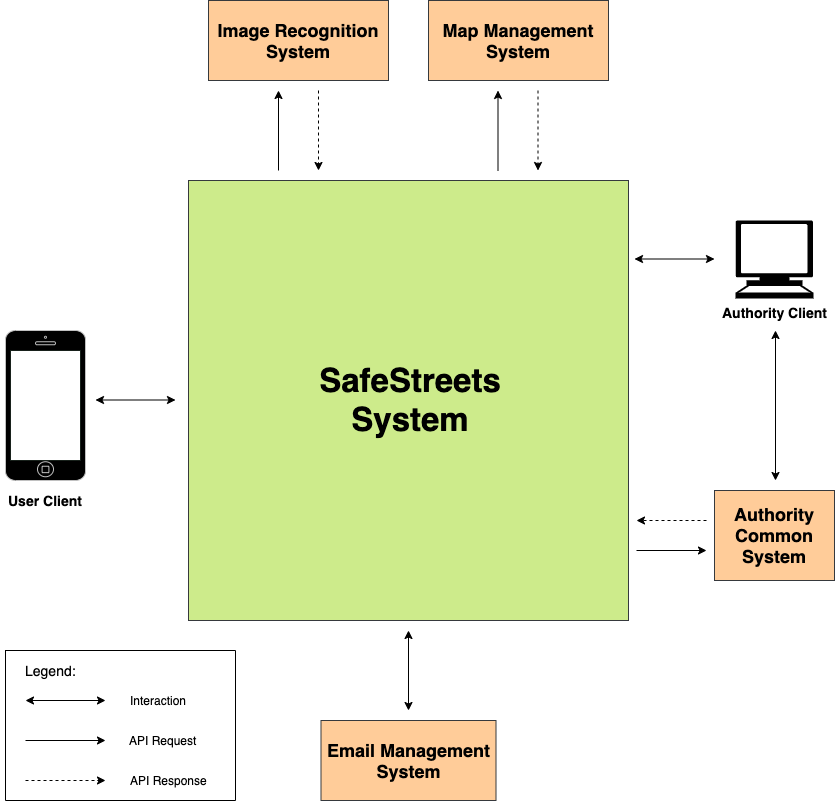
\includegraphics[scale=0.4]{miscellaneous/contextViewPoint.png}
				\caption{\label{fig:contextViewpoint} Context Viewpoint}
			\end{figure}
		
			Now that we know which are the systems needed, before dealing with the modules that will consider the communication with each of them let's understand first for which functionality they are needed for. The following table lists the three types of functionalities and a tick (\xtick) is used to express that the functionality needs the external systems services in order to be realized.
			
			\begin{center}
				\scalebox{0.64}{
					\begin{tabular}{|c|c|c|c|c|}
						\hline
						\diagbox{\textbf{Functionality}}{\textbf{System}} & Image Recognition & Map Management & Email Management & Authority Common \\ \hline
						Access & & & \xtick & \xtick \\ \hline
						Core & \xtick & \xtick & & \\ \hline
						Basic & & \xtick & & \\ \hline
						Advanced & & \xtick & & \xtick \\ \hline
					\end{tabular}
				} \captionof{table}{\label{tab:functionalityTable} System Mapping Table}
			\end{center}
		
		\subsubsection[Composition Diagram]{\hyperlink{toc}{Composition Diagram}}
			\label{sec:compositionDiagram}
			
			With the definition of the systems used by SafeStreets we are now able to highlight the modules used in order to benefit of their services. In the following diagram (\blueAutoref{fig:compositionDiagram}) we divide the system in three different types of areas, each one containing the modules considered critical for that competence.
			
			\newpage
			
			\begin{figure}[ht]
				\centering
				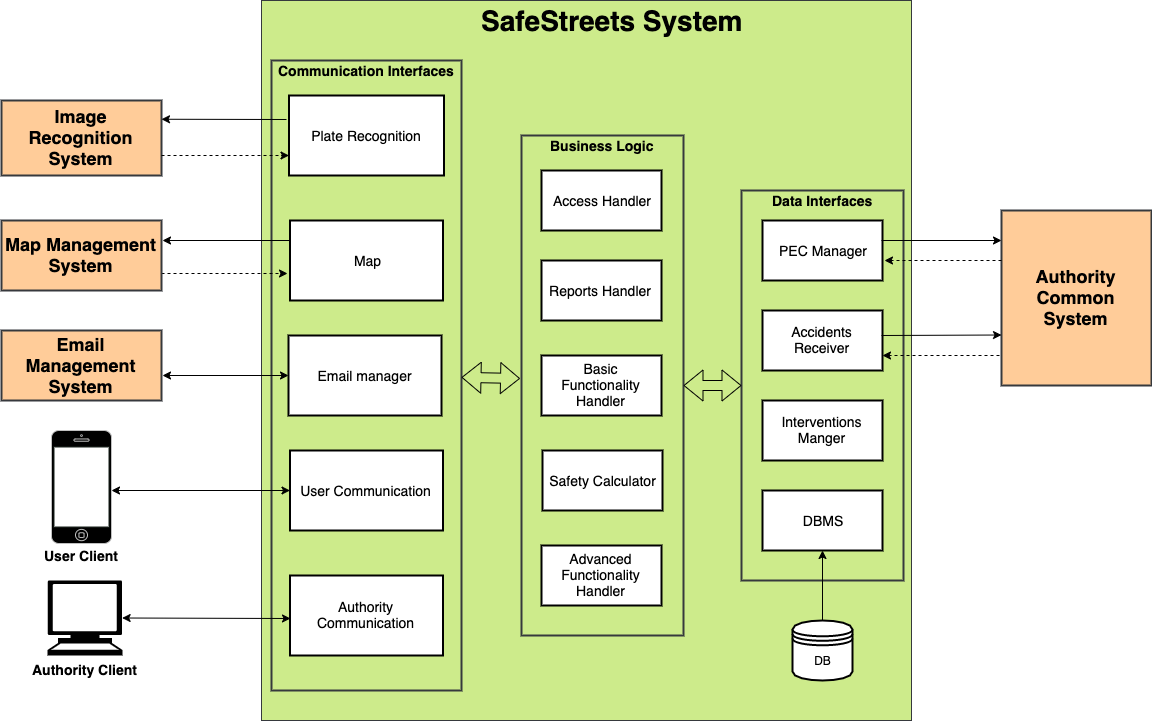
\includegraphics[scale=0.3]{miscellaneous/compositionViewPoint.png}
				\caption{\label{fig:compositionDiagram} Composition Diagram}
			\end{figure}
		
			As we see can see in the picture above, the system is composed of three areas, each one specialized on a particular behavior.
			
			\paragraph{Communication Interfaces} Are the interfaces that allows our system to interact with externally active agents or systems that provide services needed by the business logic. In fact, as we notice in the left hand-side of the diagram we have:
			
			\begin{itemize}
				\item \textbf{Image Recognition System:} provides the methods to deal with the recognition of the plate of the vehicles
				\item \textbf{Map Management System:} provides the methods to deal with all the issues related to the geographical positioning and map interaction
				\item \textbf{Email Management System:} provides the minimal email services that SafeStreets needs to consider in order to provide the recovery of the credentials and more important the recognition of the authorities
				\item \textbf{User Client:} is the client used by a user in order to benefit of SafeStreets' functionalities
				\item \textbf{Authority Client:} is the client used by an authority in order to benefit of SafeStreets' functionalities
			\end{itemize}
		
			All the modules defined here will bring inside the system all the services and requests coming from the outside as the ones in the business logic can process them and provide the functionalities.
			
			\paragraph{Business Logic} Now we have the modules that are thought to deal with the functionalities that the system has to provide. As we can see also in this case, we have a correspondence between the functionalities described in the previous section and the modules now listed:
			
			\begin{itemize}
				\item Access Handler
				\item Reports Handler
				\item Basic Functionality Handler
				\item Safety Calculator
				\item Advanced Functionality Handler
			\end{itemize}
		
			\paragraph{Data Interfaces} The last interfaces instead are separated from the initial ones because they provide a way to the system to access the external data he needs to use in order to provide its functionalities. As we can see in the right hand-side of the diagram we only have the \textbf{Authority Common Interface}: it provides the methods to retrieve the data of the accidents that took place in a certain city and the list of all the PEC addresses of the authorities.
		
	\subsection[Component View]{\hyperlink{toc}{Component View}}
		\label{sec:componentView}
		
		\begin{figure}[ht]
			\centering
			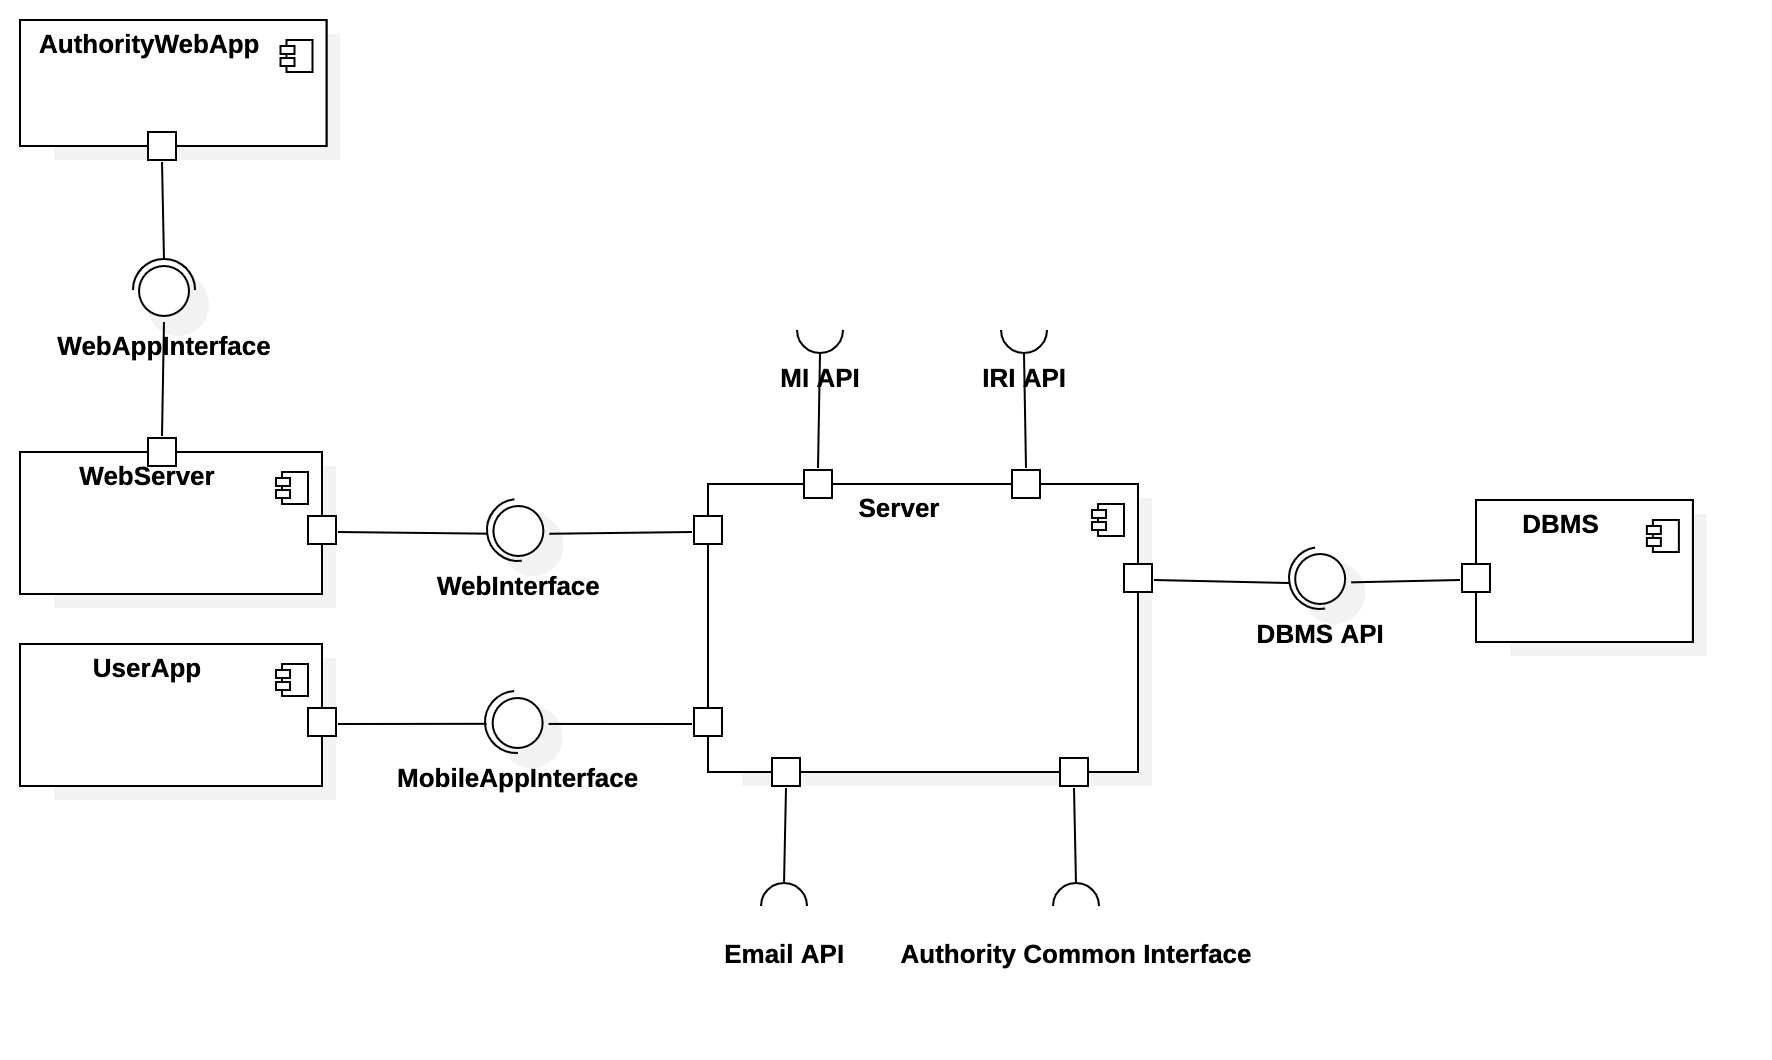
\includegraphics[scale=0.17]{/diagrams/components/highLevel.png}
			\caption{\label{fig:highLevelComp} High Level Component Diagram}
		\end{figure}
	
		With the high-level description of the system provided in the previous sections we are now able to determine which are the components that will be considered in the architecture in order to accomplish the functionalities that each of the identified modules are going to provide. In fact it is straightforward the mapping between the component diagram (\blueAutoref{fig:compositionDiagram}) and the picture above (\blueAutoref{fig:highLevelComp}). The \textbf{communication interfaces} area is mapped with all the interfaces provided by the components that provide or receive services from the outside; the \textbf{business logic} is realized by the server component where all the computation to provide the functionalities of the system takes place, while the \textbf{data interfaces} are the ones that bring to the system both the DBMS and the authority common interface's services.\\
		
		Before describing in detail the most important components of the system it is now the moment to precisely describe what are the components presented in this picture and what are the services provided by their interfaces:
		
		\begin{itemize}
			\item \textbf{Server:} it is the business logic of the entire system. Inside this component, that will be precisely described in the next section, takes place all the computation that allows to provide the customers the functionalities that SafeStreets has defined as its goals. The two interfaces provided by this components are the ones that allow the client systems to benefit of these functionalities; considering to have both a mobile application and a web app we need one interface directly for the mobile software while another interface for the web server that will provide to the browser of the authority the functionalities offered.
			
			\item \textbf{Web Interface:} it is the interface that allows the web server to access the methods that provide the functionalities once a request arrives from an authority.
			
			\item \textbf{Web Server:} it is the component that deals with all the issues related to the realization of a web app that needs to be displayed on the browser of the authority. In fact it provides the interface that  represents the endpoint where the browsers can access the system's functionalities.
			
			\item \textbf{Web App Interface:} it is the interface that allows the browsers to benefit of the services of SafeStreets with a web app technology.
			
			\item \textbf{Authority Web App:} it is the component that represents the browser used by the authority whenever it decides to access the system.
			
			\item \textbf{Mobile App Interface:} it is the interface that allows the mobile applications to access the functionalities provided by our system.
			
			\item \textbf{User App:} it is the component that represents the mobile software installed in the users' devices which accesses the services of SafeStreets thanks to the interface just presented.
			
			\item \textbf{MI API:} it is the interface that provides the methods to the system in order to deal with the map and geographical issues:
				\begin{itemize}
					\item Allows to retrieve the street providing a GPS position
					\item Allows to retrieve the best possible path between two positions
					\item Allows to display the colored map for the safety functionality
					\item Allows to store in the system all the streets and cities
				\end{itemize}
			
			\item \textbf{IRI API:} it is the interface that provides the methods to the system in order to deal with the recognition of a vehicle's plate. Remember that the algorithms accessible from this API can be helped with the information provided by the user about the plate's number and, more important, they always "have the last word": this means that whenever a result is found for the plate it will be considered correct and storable by the system; in all the cases when no result is found by the algorithms the notification will be discarded.
			
			\item \textbf{Email API:} it is the interface that provides the methods to the system in order to deal with the minimal email sending and receiving services needed. An email system in fact is necessary both for the process of code verification to recognize the authorities and also for the credential recovery of both the customers.
			
			\item \textbf{Authority Common Interface:} it is the interface that provides the methods to the system in order to deal with the PEC addresses and the accidents receiving. This interface is thought to be provided by a common system used by every authority, where:
			
			\begin{itemize}
				\item we can retrieve all the PEC addresses of each authority, in order to do the checks in the recognition process
				\item we can retrieve all the accidents that took place in the area of an authority's competence. It is assumed that the exchange of the accidents' data develops in this way: each authority publishes its accidents on the common system as we can periodically try to retrieve them.
			\end{itemize}
		
			\item \textbf{DBMS API:} it is the interface that provides the methods to the system in order to deal with the data management process. Starting from the access one, the notification process and all the others that need to require or store information from the database of the system (in the following section it will be clear which are the components that necessarily need to access the DBMS interface).
			 
		\end{itemize}
	
		\subsubsection[Server Component]{\hyperlink{toc}{Server Component}}
			\label{sec:serverComponent}
			
			From now on we are going to blow up the high-level component view just presented, starting with the most complex component that is the server and continuing first with its internal ones and in the end with the others that we have to take into account while defining the architecture of our system (WebServer and UserApp). In all the diagrams we are going to illustrate, the interaction between the components and the interfaces provided is carried on by means of the lollipop-socket notation. We will then continue by precisely describing each of these components to understand how they allow to obtain the functionalities of the system by providing and using the interfaces identified.\\
			
			The diagram of the next page (\blueAutoref{fig:serverComp}) highlights all the components that compose the server and describes both their internal and external interactions: we can see in fact how the interfaces that we defined in the previous section are provided or used by these components and how new interfaces are needed to make them interact.
			
			\begin{figure}[h!]
				\centering
				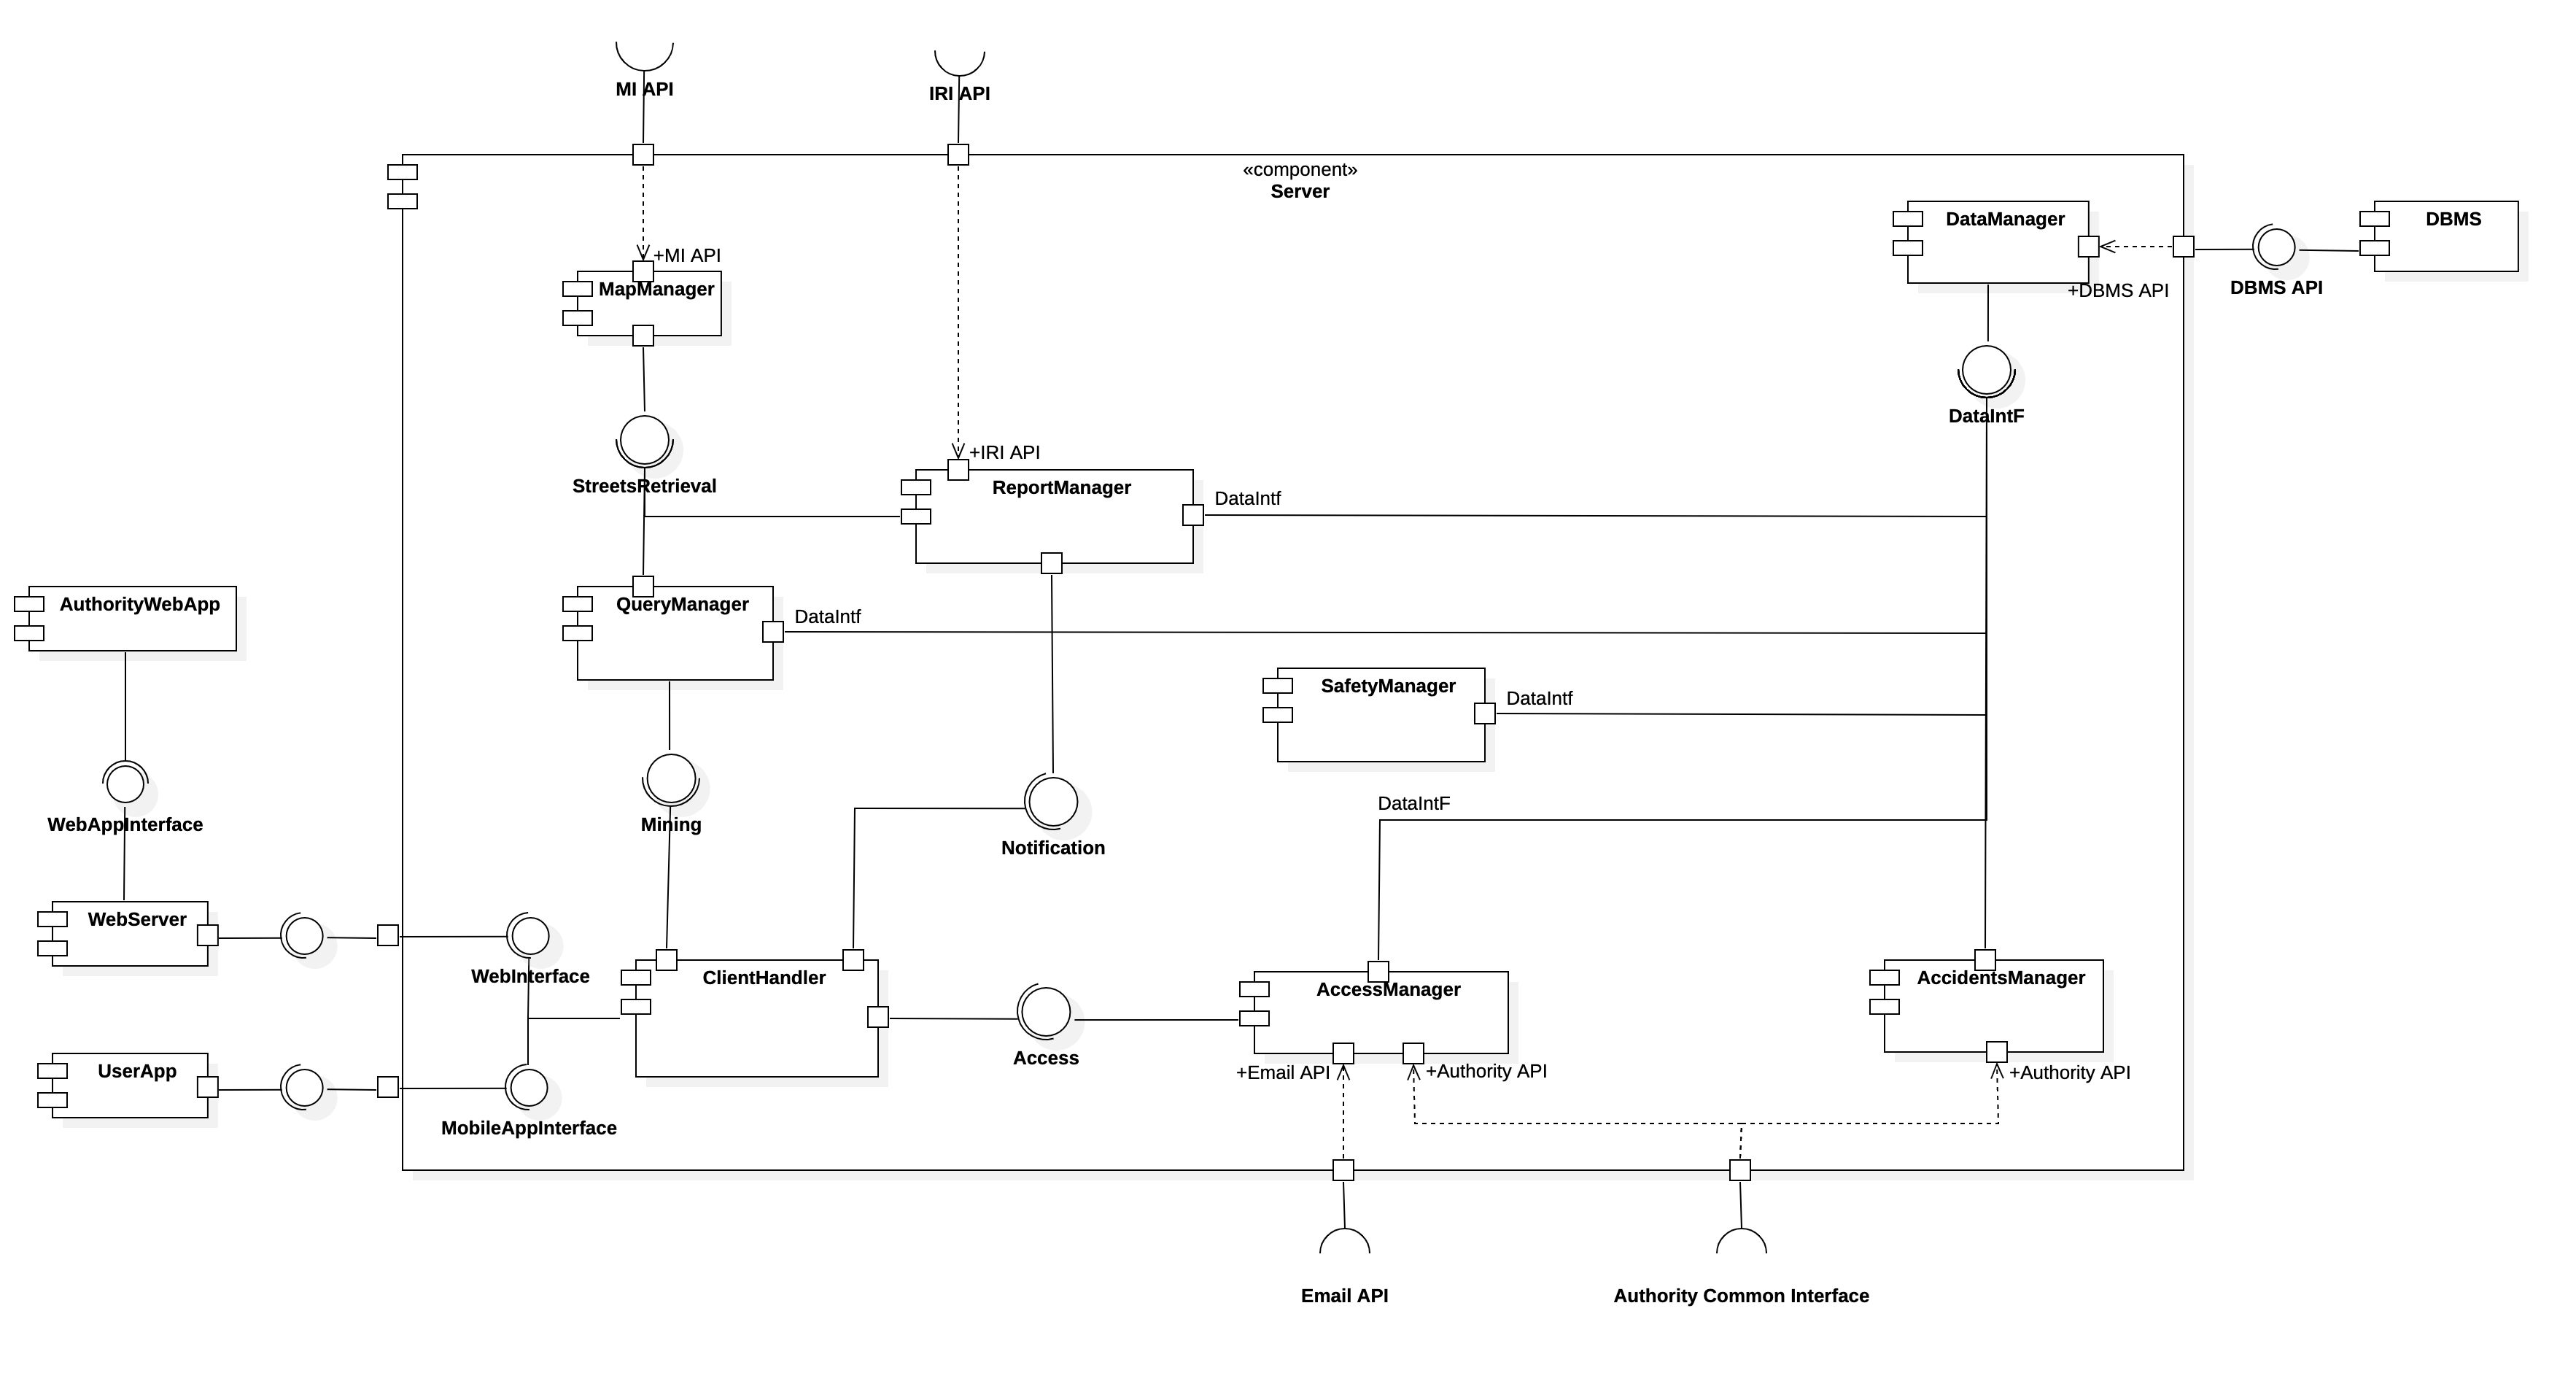
\includegraphics[scale=0.16, angle=90]{/diagrams/components/server.png}
				\caption{\label{fig:serverComp} Server Component Diagram}
			\end{figure}
		
			\FloatBarrier 
		
		\subsubsection[Client Handler Component]{\hyperlink{toc}{Client Handler Component}}
			\label{sec:clientHandlerComponent}
			
			The \emph{ClientHandler} (\blueAutoref{fig:clientHandlerComp}) is the component that manages all the requests coming from the customers. As we see, two interfaces are provided, one for the mobile application (\textbf{MobileAppInterface}) and the other for the web server, that manages the web application (\textbf{WebInterface}). These two interfaces are the ones that extend the general \textbf{HandleRequest} to define a more precise communication with the components of the clients. It is important to understand that this approach, as precisely described in the section \blueRef{sec:selectedArchitecturalStylesAndPatterns}, allows us to use one single technology to interact with both the mobile and the web applications: this simplifies both the maintenance and replacement of the interface and it gives also lots of advantages in the IIT plan. In the component interfaces diagram (\blueAutoref{fig:componentInterfaces}) we will describe the \textbf{WebInterface} and the \textbf{MobileAppInterface} but we have to remember that they are the extension of the most general \textbf{HandleRequest} interface defined in this component.
			
			\begin{figure}[h!]
				\centering
				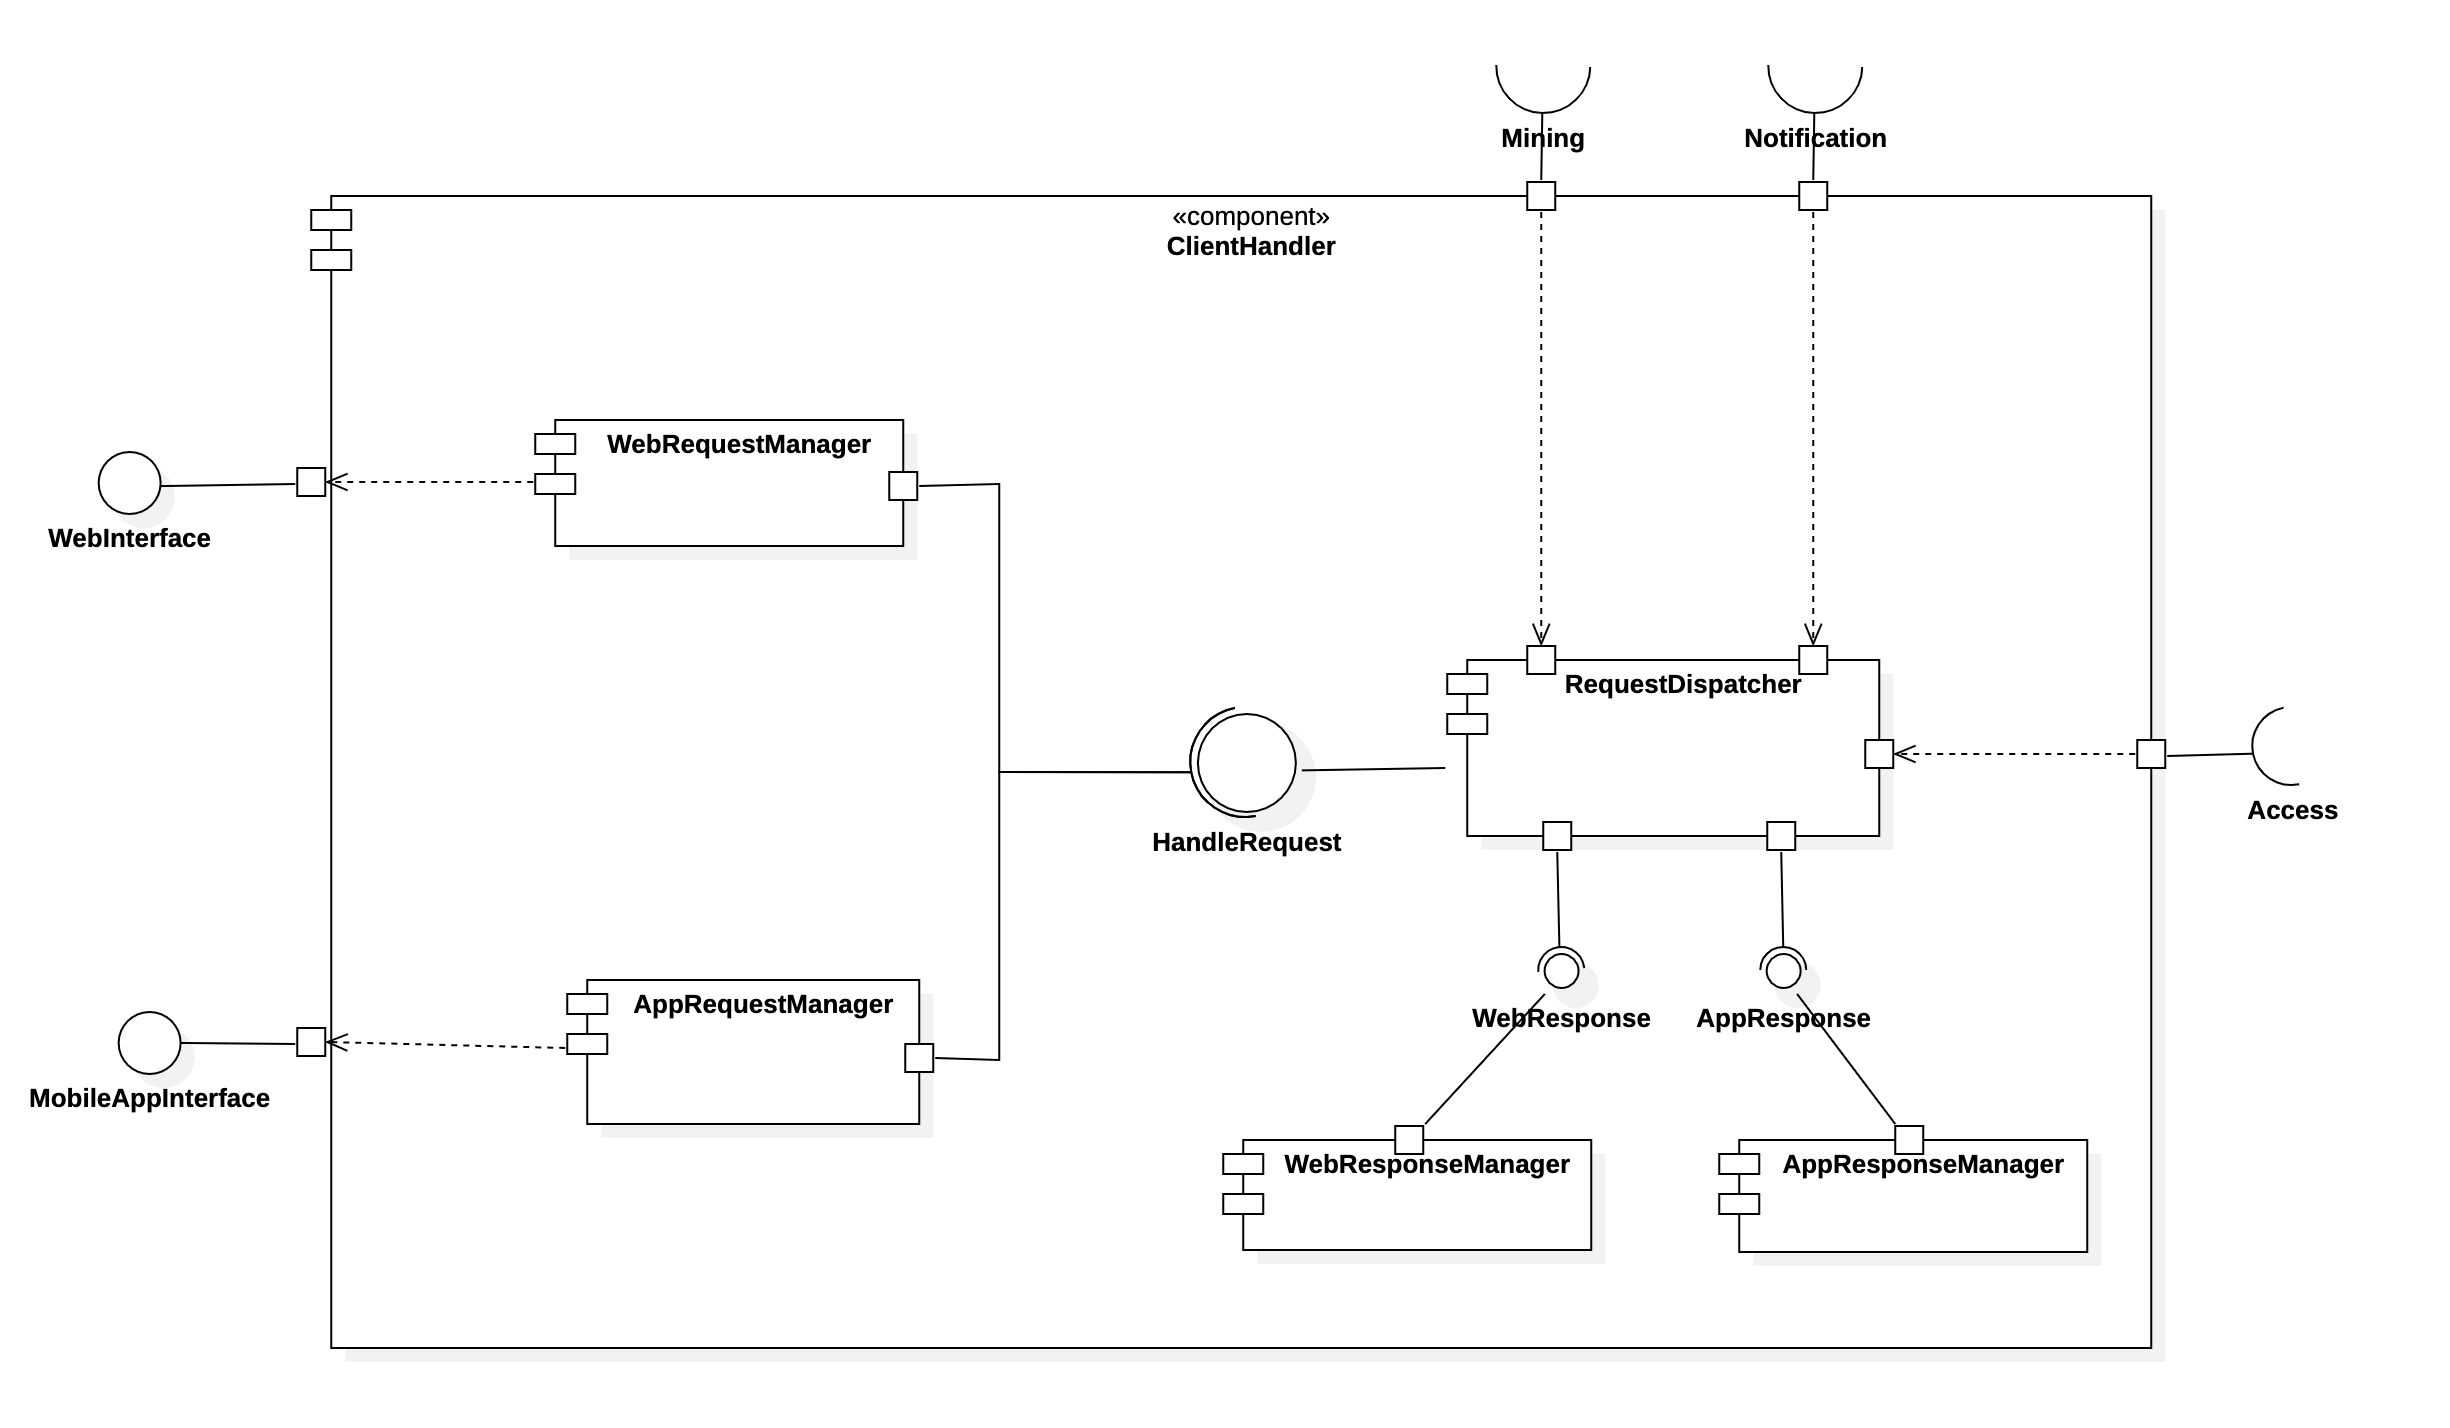
\includegraphics[scale=0.15]{/diagrams/components/clientHandler.png}
				\caption{\label{fig:clientHandlerComp} Client Handler Component Diagram}
			\end{figure}
			
			The components that allow the \emph{ClientHandler} to process a request, first receiving it and then dispatching it to the related functionality are:
			
			\begin{itemize}
				\item \textbf{RequestDispatcher:} it is the component that allows to handle each type of request that comes either from the web app or the mobile one. In fact, thanks to the \textbf{HandleRequest Interface} the components previously described can deploy the request to this one that, depending on the type of the request, will need to use different services in order to provide the functionality required. As a consequence, we can see several interfaces that are used by this component:
				
				\begin{itemize}
					\item \textbf{Mining Interface:} allows to benefit of the methods provided by the \emph{QueryManager} component that is the one which manages all the queries related to the basic and the advanced functionalities.
					
					\item \textbf{Notification Interface:} it is the interface that allows to manage the notification process once a request to report a parking violation is sent by a user.
					
					\item \textbf{Access Interface:} it is the interface that allows to deal with all the issues related to the access to the system. This means: the login, the registration, the credential recovery, the recognition of the authorities...
					
					\item \textbf{WebResponse Interface:} it is the interface that allows to process the information received from the logic of the system as it can be used by the \emph{WebServer} to be displayed on the web app.
					
					\item \textbf{MobileResponse Interface:} it is the interface that allows to process the information received from the logic of the system as it can be used by the device to be displayed on the mobile app.
				\end{itemize}
			\end{itemize}
		
		\subsubsection[Access Manager Component]{\hyperlink{toc}{Access Manager Component}}
			\label{sec:accessManagerComponent}
			
			The \emph{AccessManager} (\blueAutoref{fig:accessManagerComp}) is the component that manages all the issues related to the access of the customers. As we have said several times when defining the goals and requirements of SafeStreets, in fact, it is fundamental to recognize the clients and thus to provide a registration process.\\
			
			The components described in the following diagram are the ones that allow to provide the access functionalities of:
			
			\begin{itemize}
				\item Registration
				\item Login
				\item Credentials Recovery
			\end{itemize}
		
			In order to provide the methods that allow to realize these functionalities through the \textbf{Access Interface}, this component has also to benefit of the external services provided by the \textbf{Email API} and the \textbf{Authority API}. The interface that allows to access and manage the data stored in the system is obviously fundamental for all the checks needed and to store new customers in the application.\\
			
			The components that allow the \emph{AccessManager} to process an access request, meaning one of the three functionalities listed before are:
			
			\begin{itemize}
				\item \textbf{Email Manager:} it is the component that uses the methods provided by the \textbf{Email API} in order to have a way to send the emails with the recognition code and to offer the service of the credentials recovery. This component provides the \textbf{mail Interface} to expose the methods related to its service.
			
				\item \textbf{PEC Manager:} it is the component that deals with all the issues related to the PEC addresses. In fact it uses the methods provided by the \textbf{Authority API} in order to know which are the existing addresses of all the authorities and then uses the \textbf{mail Interface} to provide through the \textbf{PEC Interface} the methods that allow to send the verification code in the registration process.
			\end{itemize}
			
			\begin{figure}[ht]
				\centering
				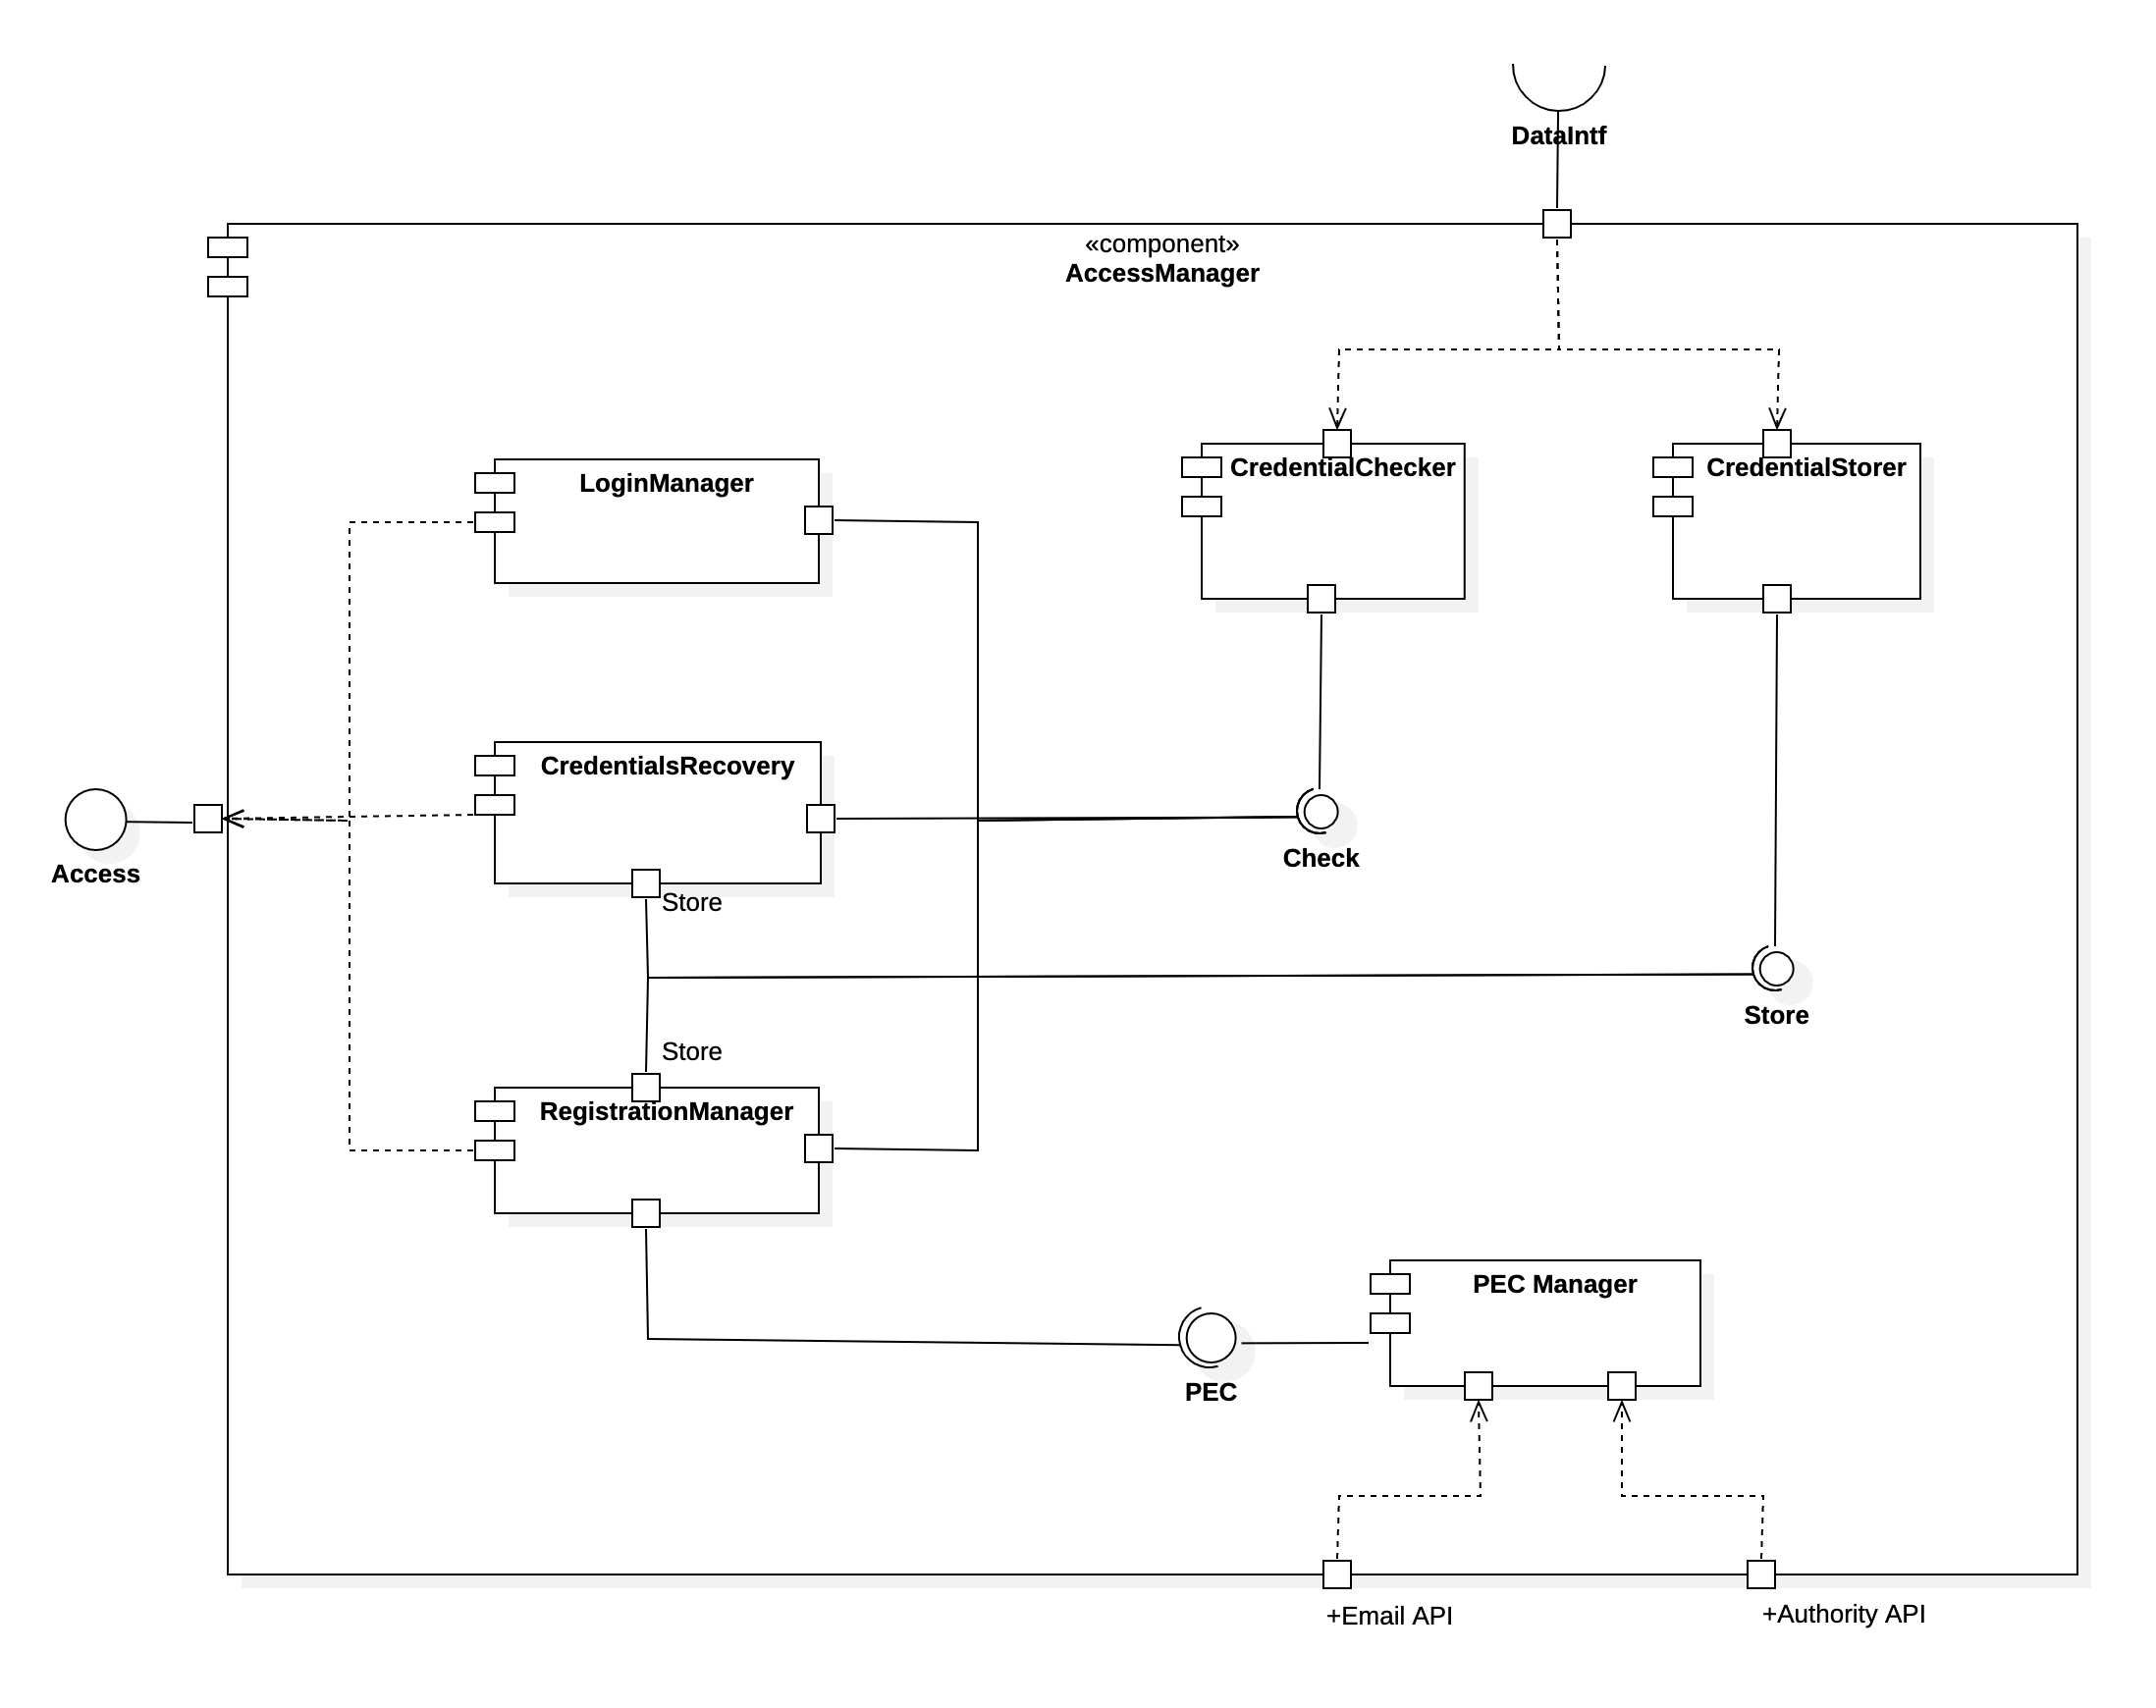
\includegraphics[scale=0.16]{/diagrams/components/accessManager}
				\caption{\label{fig:accessManagerComp} Access Manager Component Diagram}
			\end{figure}
		
			\begin{itemize}
				\item \textbf{LoginManager:} it is the component that deals with the login process. It realizes the \textbf{Access Interface} by providing the methods for the login and has always to interact with the \emph{CredentialChecker} component in order to verify the credentials of the logging customer. In this way, thanks to the \textbf{Check Interface}, this component will control the credential of either the user or the authority and decide if to authenticate them or not.
				
				\item \textbf{CredentialRecovery:} it is the component that deals with the credentials recovery process. It realizes the \textbf{Access Interface} by providing the methods for the recovery and thus it needs to interact with both the \emph{CredentialChecker} and the \emph{CredentialStorer} components. Thanks to the \textbf{Check Interface} and the \textbf{Store Interface}, in fact, it will be able to control the identity of the customer who is requiring to recover its credentials and store its possible new information. Obviously the \textbf{mail Interface} is also needed in order to send the email to the client that is requiring to recover its credentials.
				
				\item \textbf{RegistrationManager:} it is the component that deals with the registration of the customers. It realizes the \textbf{Access Interface} by providing the methods to register both the user and the authority and thus needs to use the \textbf{Check Interface} and the \textbf{Store Interface}. In fact, this component will need to check for the new credentials to be feasible and then to store the new data related to the registering customer. The \textbf{PEC Interface} is used for the authority registration process to send the verification code and check the address.
				
				\item \textbf{CredentialsChecker:} it is the component that deals with all the checks needed in the access functionalities previously described by providing the \textbf{Check interface}. Obviously to perform these checks it needs to access the database of the system and thus the methods provided by the \textbf{DataIntF Interface}.
				
				\item \textbf{CredentialStorer:} it is the component that deals with the storing of all the data used in the access functionalities by providing the \textbf{Store Interface}.
				Obviously in order to store the information in the database it needs to use the methods provided by the \textbf{DataIntF Interface}.
			\end{itemize}
		
		\subsubsection[Query Manager Component]{\hyperlink{toc}{Query Manager Component}}
			\label{sec:queryManagerComponent}
			
			The \emph{QueryManager} (\blueAutoref{fig:queryManagerComp}) is the component that manages the requests related either to the basic or the advanced functionalities (see section \blueRef{sec:generalContext} for the precise functionalities description) coming from the customers with the realization of the \textbf{Mining Interface}. Hence, this component needs first to identify the request, then it checks its filters with the \textbf{Check Interface} and finally, once identified the functionality, it realizes the respective query with the relative interface provided by the correct component:
			
			\begin{itemize}
				\item Interventions Interface
				\item Safety Interface
				\item Reports Interface
				\item Dangerous Interface
				\item Frequency Interface
			\end{itemize}
		
			Once the query is ready it is prepared and sent to the component that will execute it through the \textbf{Send Interface} realized by the \emph{QuerySender}.\\
			
			The components that allow the \emph{QueryManager} to process the requests related to a functionality are:
			
			\begin{itemize}
				\item \textbf{FunctionalityIdentifier:} it is the components that realizes the \textbf{Mining Interface} by providing the methods related to the processing of a request that deals with one of the basic or advanced functionalities. This component first needs to recognize which is the functionality requested as it can check it and then prepare it to be executed. Thanks to the \textbf{Check Interface} it controls if the filters in the request are feasible with the ones related to the functionality recognized and then it calls the method that builds the query from the correct interface between the ones presented before.
			\end{itemize}
			
			\begin{figure}[ht]
				\centering
				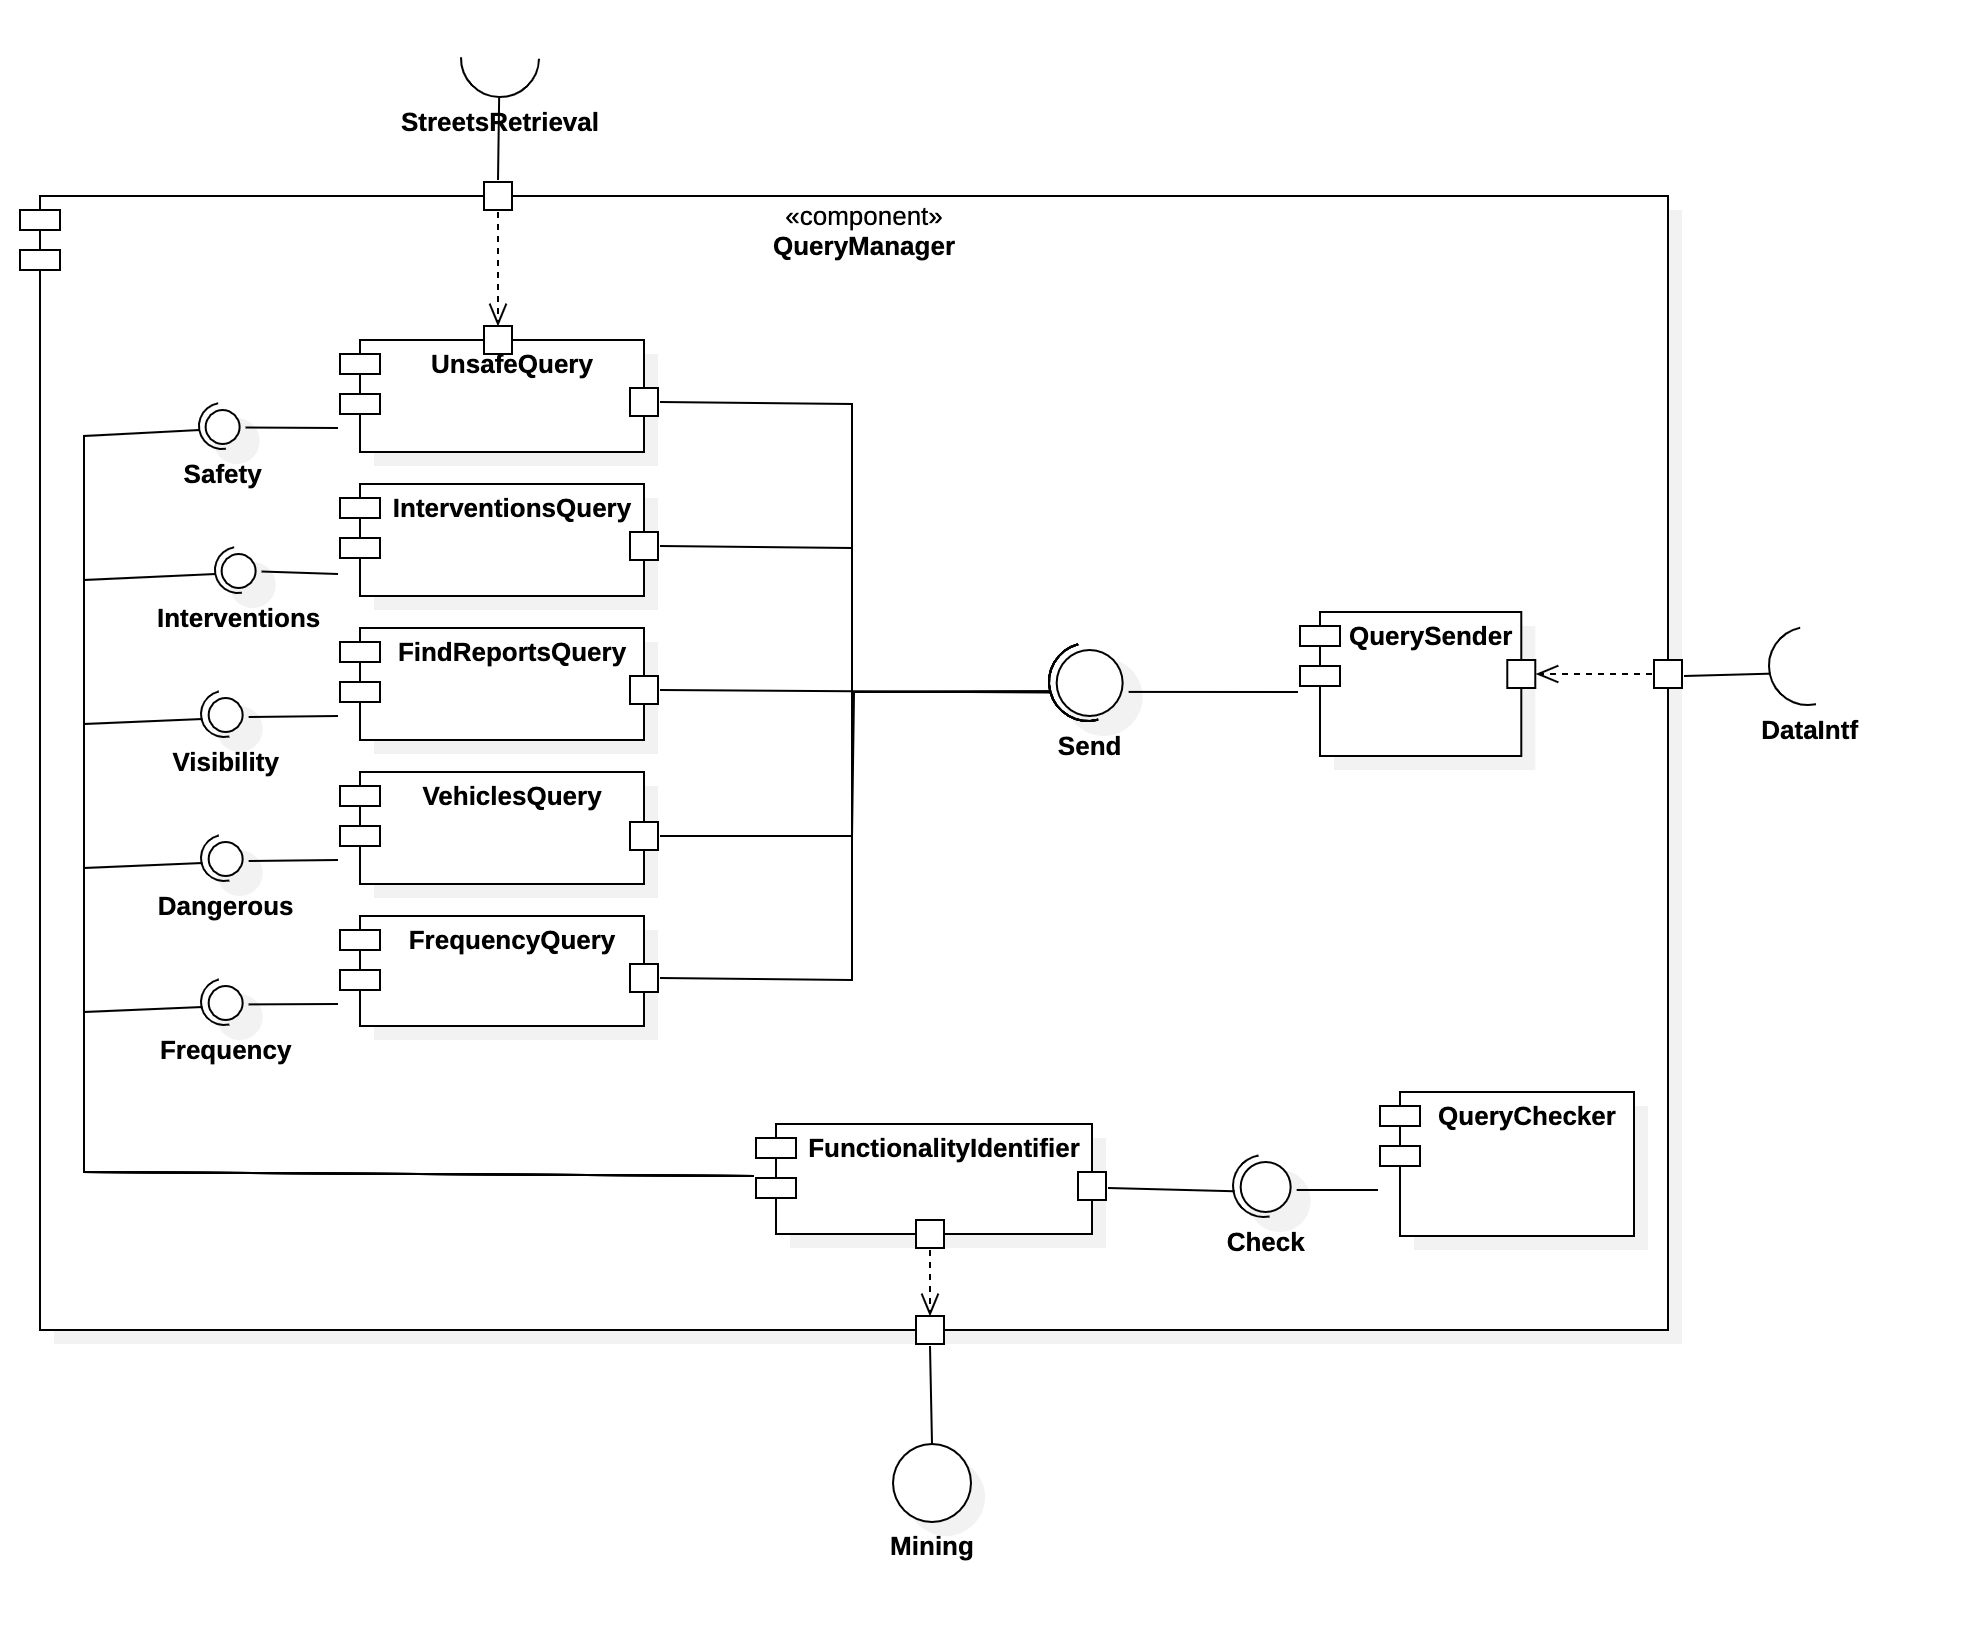
\includegraphics[scale=0.2]{/diagrams/components/queryManager.png}
				\caption{\label{fig:queryManagerComp} Query Manager Component Diagram}
			\end{figure}
		
			\begin{itemize}
				\item \textbf{UnsafeQuery:} it is the component that manages the query related to the safety functionality. Hence it will select the correct area and retrieve the safety of all the streets required by the customer as they can be displayed on the map. This component realizes the \textbf{Safety Interface} and needs to use the methods provided by the \textbf{StreetsRetrieval Interface}. The path retrieval and the JSON file that will be used to display the map are the result of an invocation of one of the methods of the last interface presented.
				
				\item \textbf{InterventionsQuery:} it is the component that manages the query related to the suggestion for possible interventions functionality. Hence it will prepare the query over the city selected and retrieve all the suggestions for it. This component realizes the \textbf{Interventions Interface} used by the \emph{FunctionalityIdentifier}.
				
				\item \textbf{ReportsRetrieverQuery:} it is the component that manages all the functionalities that require to retrieve the reports from a request made by an authority. For this reason it handles both the \emph{Check Unread Reports} and \emph{Find Reports} functionalities provided to the authorities, that are nothing more than a query over the database retrieving the violations. 
				
				\begin{itemize}
					\item \textbf{Check Unread Reports:} it is the functionality that allows the authority to be notified of new parking violations. Thanks to the unread flag that is stored in the system whenever a new notification is accepted we are able to retrieve for every authority its notifications and display them for this functionality.
					
					\item \textbf{Find Reports:} it is the functionality that provides the authority with a different level of visibility the retrieval of the notifications. In fact, while the user is able to see only some statistics thanks to the basic functionalities, in this way the authorities are able to see in detail each of the reports of their competence.
				\end{itemize}
			
				This component realizes the \textbf{Reports Interface} used by the \emph{FunctionalityIdentifier}.
				
				\item \textbf{VehiclesQuery:} it is the component that manages the query related to the dangerous vehicles functionality. Hence it will prepare the query with the filters already checked and retrieve the type of dangerous vehicles. This component realizes the \textbf{Dangerous Interface} used by the \emph{FunctionalityIdentifier}.
				
				\item \textbf{FrequencyQuery:} it is the component that manages the query related to the violations frequency functionality. Hence it will prepare the query with the filters already checked and retrieve the streets with most violations. This component realizes the \textbf{Frequency Interface} used by the \emph{FunctionalityIdentifier}.
				
				\item \textbf{QuerySender:} it is the component that allows to send the query to the \emph{DataManager}. Thanks to the \textbf{Send Interface}, in fact, the five components just presented will send the query they have prepared to the \emph{DataManager} who will execute it over the database of the system.
			\end{itemize}
		
		\subsubsection[Report Manager Component]{\hyperlink{toc}{Report Manager Component}}
			\label{sec:reportManagerComponent}
			
			The \emph{ReportManager} (\blueAutoref{fig:reportManagerComp}) is the component that manages the notification process of the system, hence the one that we called the core functionality of SafeStreets. We have to remark that the notification process starts when a report arrives from a user and then the methods of the \textbf{Notification Interface} are invoked and ends when all the information about the report are stored in the system. At the end of the process each notification stored is marked as unread as it can be retrieved by the competent authority whenever it requires to benefit of the check unread reports functionality.\\
			
			As we have already said in the description of the functionality we will need to complete the data provided by the user with some controls and additions that will be performed thanks to the three interfaces that we can see are used by this component:
			
			\begin{itemize}
				\item StreetRetrieval Interface
				\item IRI API
				\item DataIntF Interface
			\end{itemize}
		
			The components that allow the \emph{ReportManager} to handle the notification process are:
			
			\begin{itemize}
				\item \textbf{ReportValidator:} it is the main component that deals with the notification process of the user-side. Once a report is notified by a user, all the information related to it will be delivered to this component by the \emph{ClientHandler} thanks to the \textbf{Notification Interface}. Before storing the information, it has to be managed in order to add the missing details and validate its content; these two further considerations are managed with the methods provided by these interfaces:
				
				\begin{itemize}
					\item \textbf{HandlePosition:} it is the interface that retrieves the street providing the GPS position of where the parking violation occurred.
					
					\item \textbf{PlateRecognition:} it is the interface that retrieves the plate of the reported vehicle providing the images of the infraction and the possible additional number inserted by the user. It is important to remark once more that the result of the methods provided by this interface will determine whether to discard or not the notification.
					
					\item \textbf{Check:} it is the interface that allows to check if there exists already the same notification in the system. As we have already said, it is useless to store twice the same notification, in the case of a duplicate the current one will be discarded.
					
					\item \textbf{Store:} it is the interface that allows to store the notification once the data completion and the validity have been carried out by the components.
				\end{itemize}
			\end{itemize}
			
			\begin{figure}[ht]
				\centering
				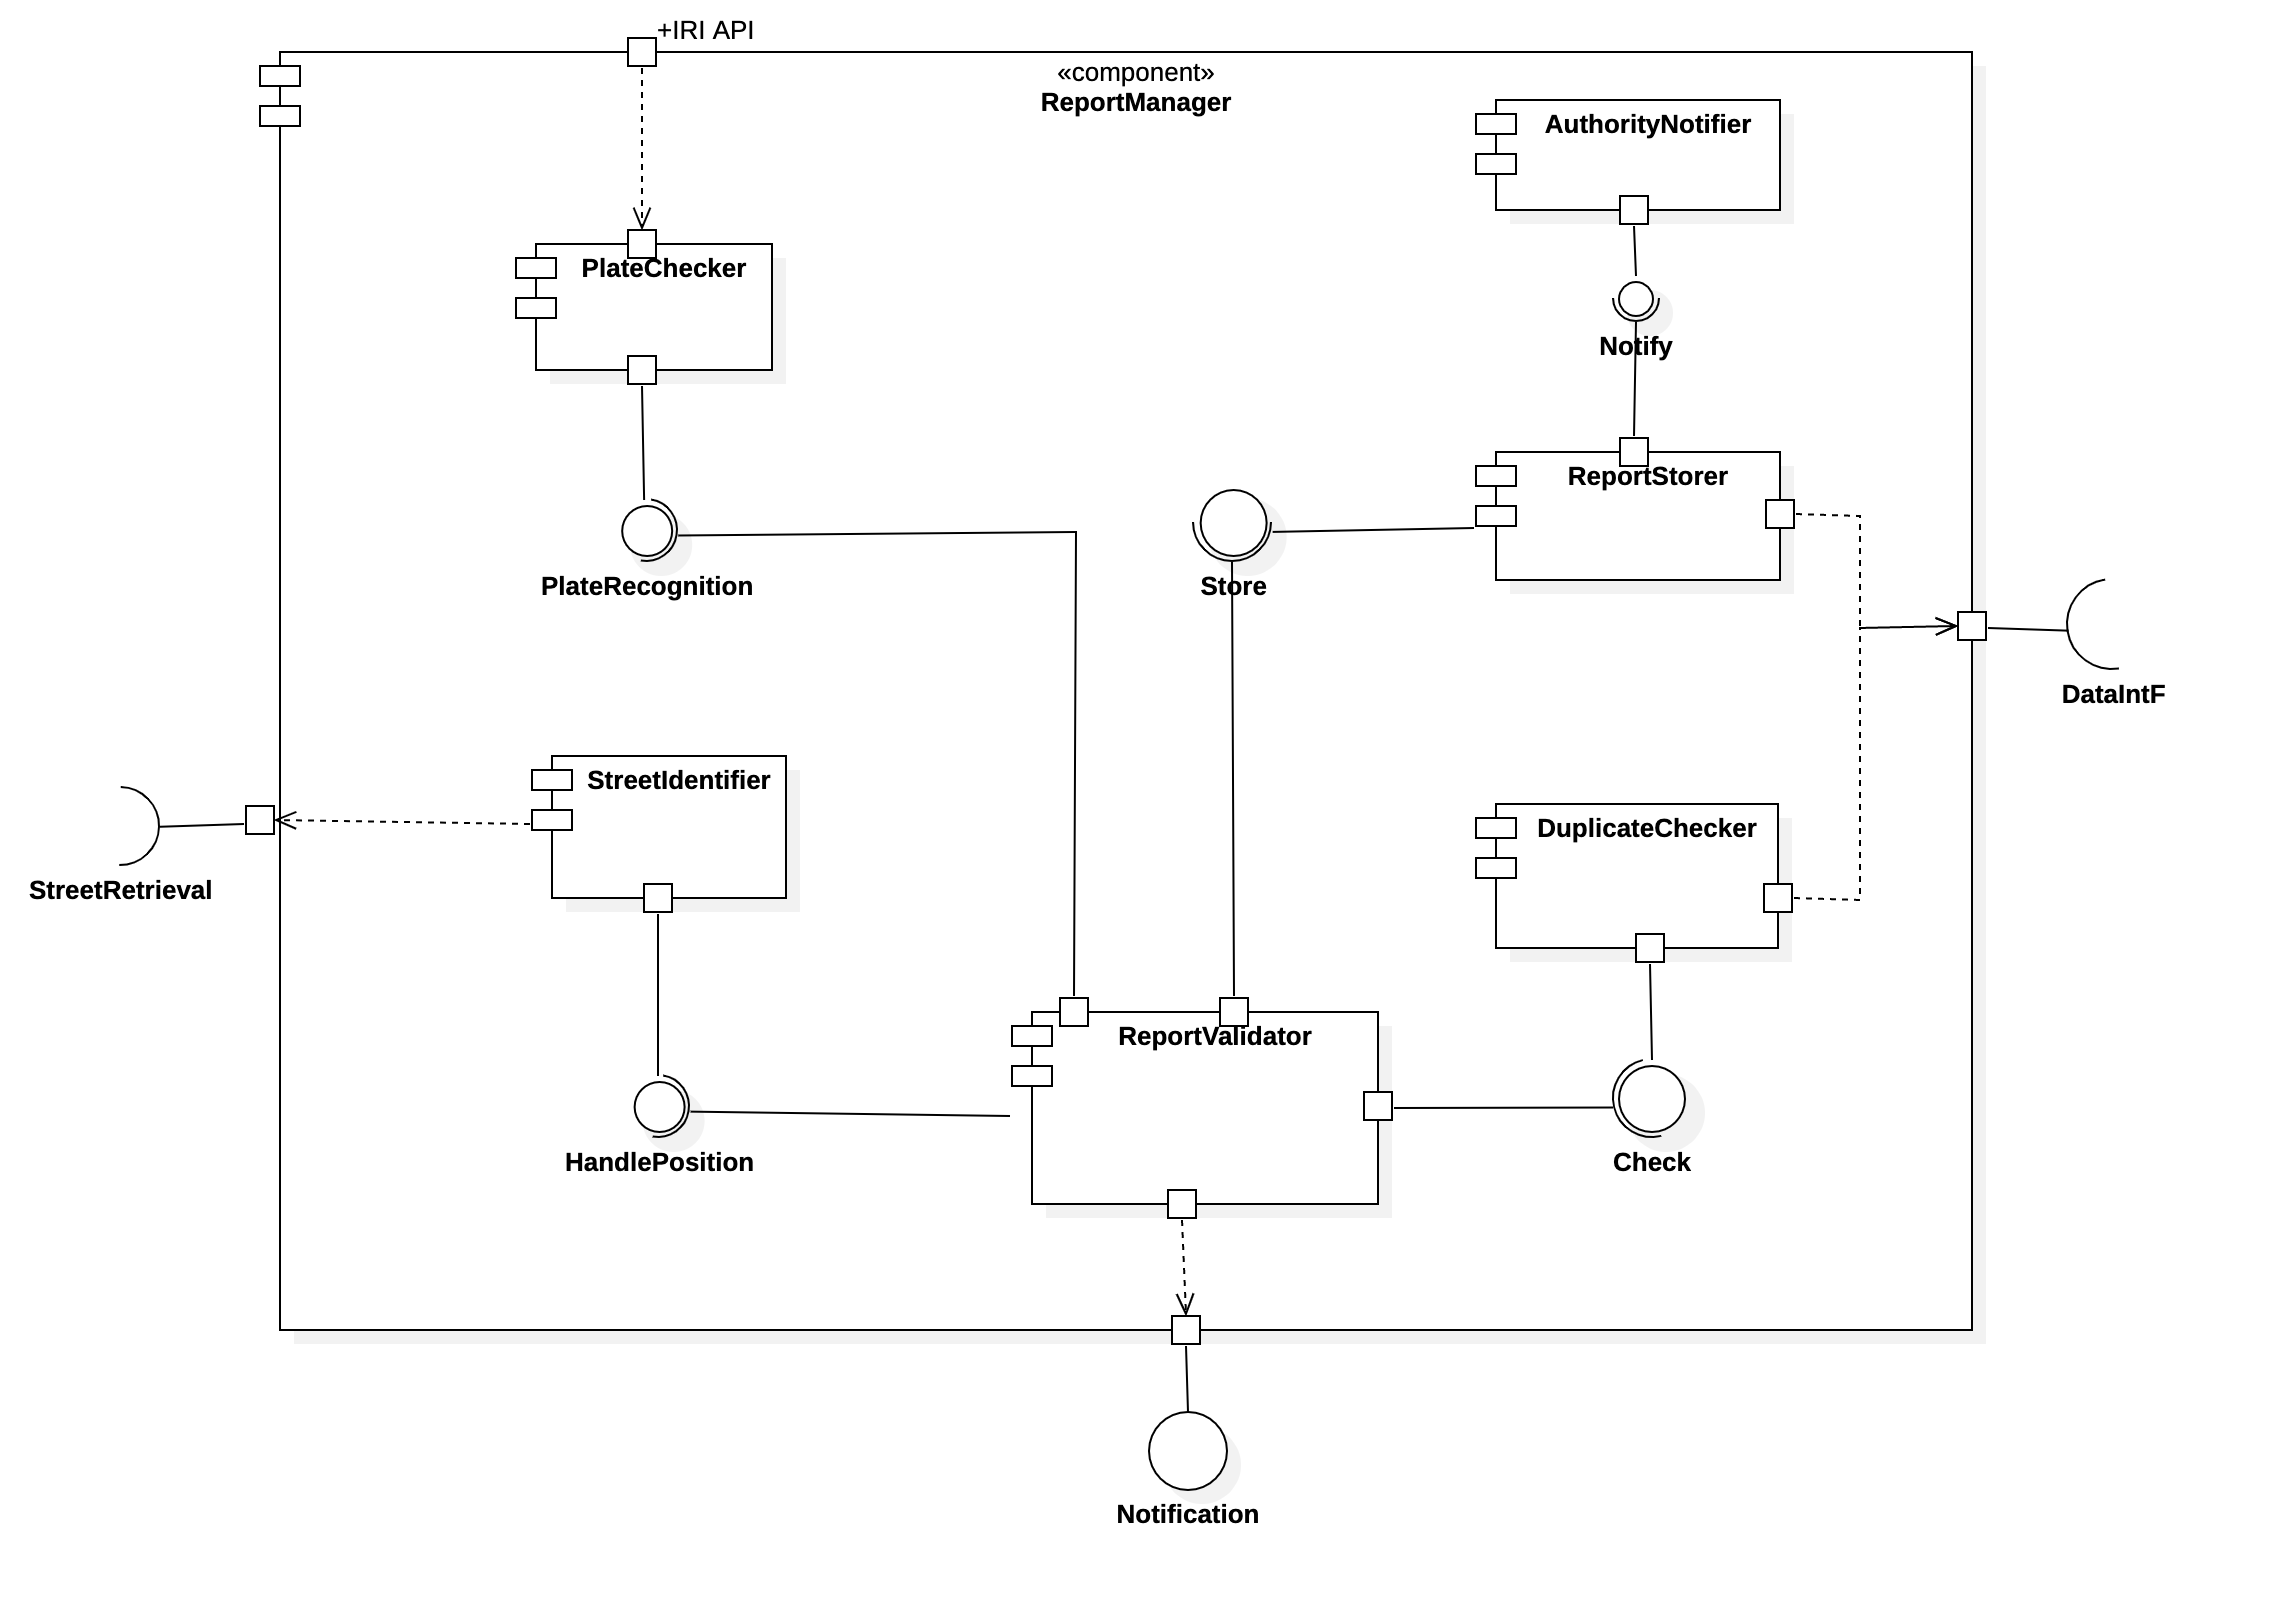
\includegraphics[scale=0.17]{/diagrams/components/reportManager.png}
				\caption{\label{fig:reportManagerComp} Report Manager Component Diagram}
			\end{figure}
		
			\begin{itemize}
				\item \textbf{Street Identifier:} it is the component that manages to retrieve the street where the violation occurred using the GPS position provided in the notification. This component realizes the \textbf{HandlePosition Interface} thanks to the methods provided by the \textbf{StreetsRetrieval Interface}. These are the real ones that execute the algorithms provided by the external map management system.
				
				\item \textbf{PlateReader:} it is the component that runs the algorithms provided by the IRI API in order to recognize the plate of the vehicle reported. It realizes the \textbf{PlateRecognition Interface} that is used to benefit of this result, fundamental to validate the notification.
				
				\item \textbf{DuplicateChecker:} it is the component that manages to check whether the reported violation is already stored in the database or not. It realizes the \textbf{Check Interface} which provides the methods to perform this additional control before storing the notification.
				
				\item \textbf{ReportStorer:} it is the component that manages to store the notification once it is ready (remember the unread flag). It realizes the \textbf{Store Interface} and uses the methods provided by the \textbf{DataIntF Interface} in order to store the data relative to the reporting notification.
			\end{itemize}
		
		\subsubsection[Map Manager Component]{\hyperlink{toc}{Map Manager Component}}
			\label{sec:mapManagerComponent}
			
			The \emph{MapManager} (\blueAutoref{fig:mapManagerComp}) is the component that deals with all the map issues. We have already presented them while describing the MI API (section \blueRef{sec:componentView}); we are going to see now the components that manage these issues thanks to the methods provided by the external map management system. The functionalities of SafeStreets will be managed by the other components using the methods provided by the \textbf{StreetsRetrieval Interface} realized by this component.\\
			
			The components that allow the \emph{MapManager} to handle all the geographical and map issues inside the system are:
			
			\begin{itemize}
				\item \textbf{StreetFinder:} it is the component that allows to retrieve the street where the parking violation occurred once the GPS position is provided. It realizes the \textbf{StreetsRetrieval Interface} thanks to the methods provided by the \textbf{GPS Interface}.
				
				\item \textbf{GPSPositionHandler:} it is the component that runs the algorithms provided by the MI API in order to realize the \textbf{GPS Interface}.
				
				\item \textbf{MapRequest:} it is the component that deals both with the retrieval of the best path between two positions provided by the customer and the mapping of each street with the correspondent safety. The shortest path is managed with the methods provided by the \textbf{Path Interface} while the mapping is carried by the the methods of the \textbf{Map Interface}. 
							
				\item \textbf{ShortestPathHandler:} it is the component that runs the algorithms provided by the MI API in order to realize the \textbf{Path Interface}.
				
				\item \textbf{MapUpdater:} it is the component that allows the system to have the information of all the streets and cities it has to manage inside its database. It Thanks to this information provided by the MI API, this component will periodically ask if some updates have occurred on the maps and in case store them inside the database thanks to the interaction with the \textbf{DataIntF Interface}.
			\end{itemize}
			
			\begin{figure}[ht]
				\centering
				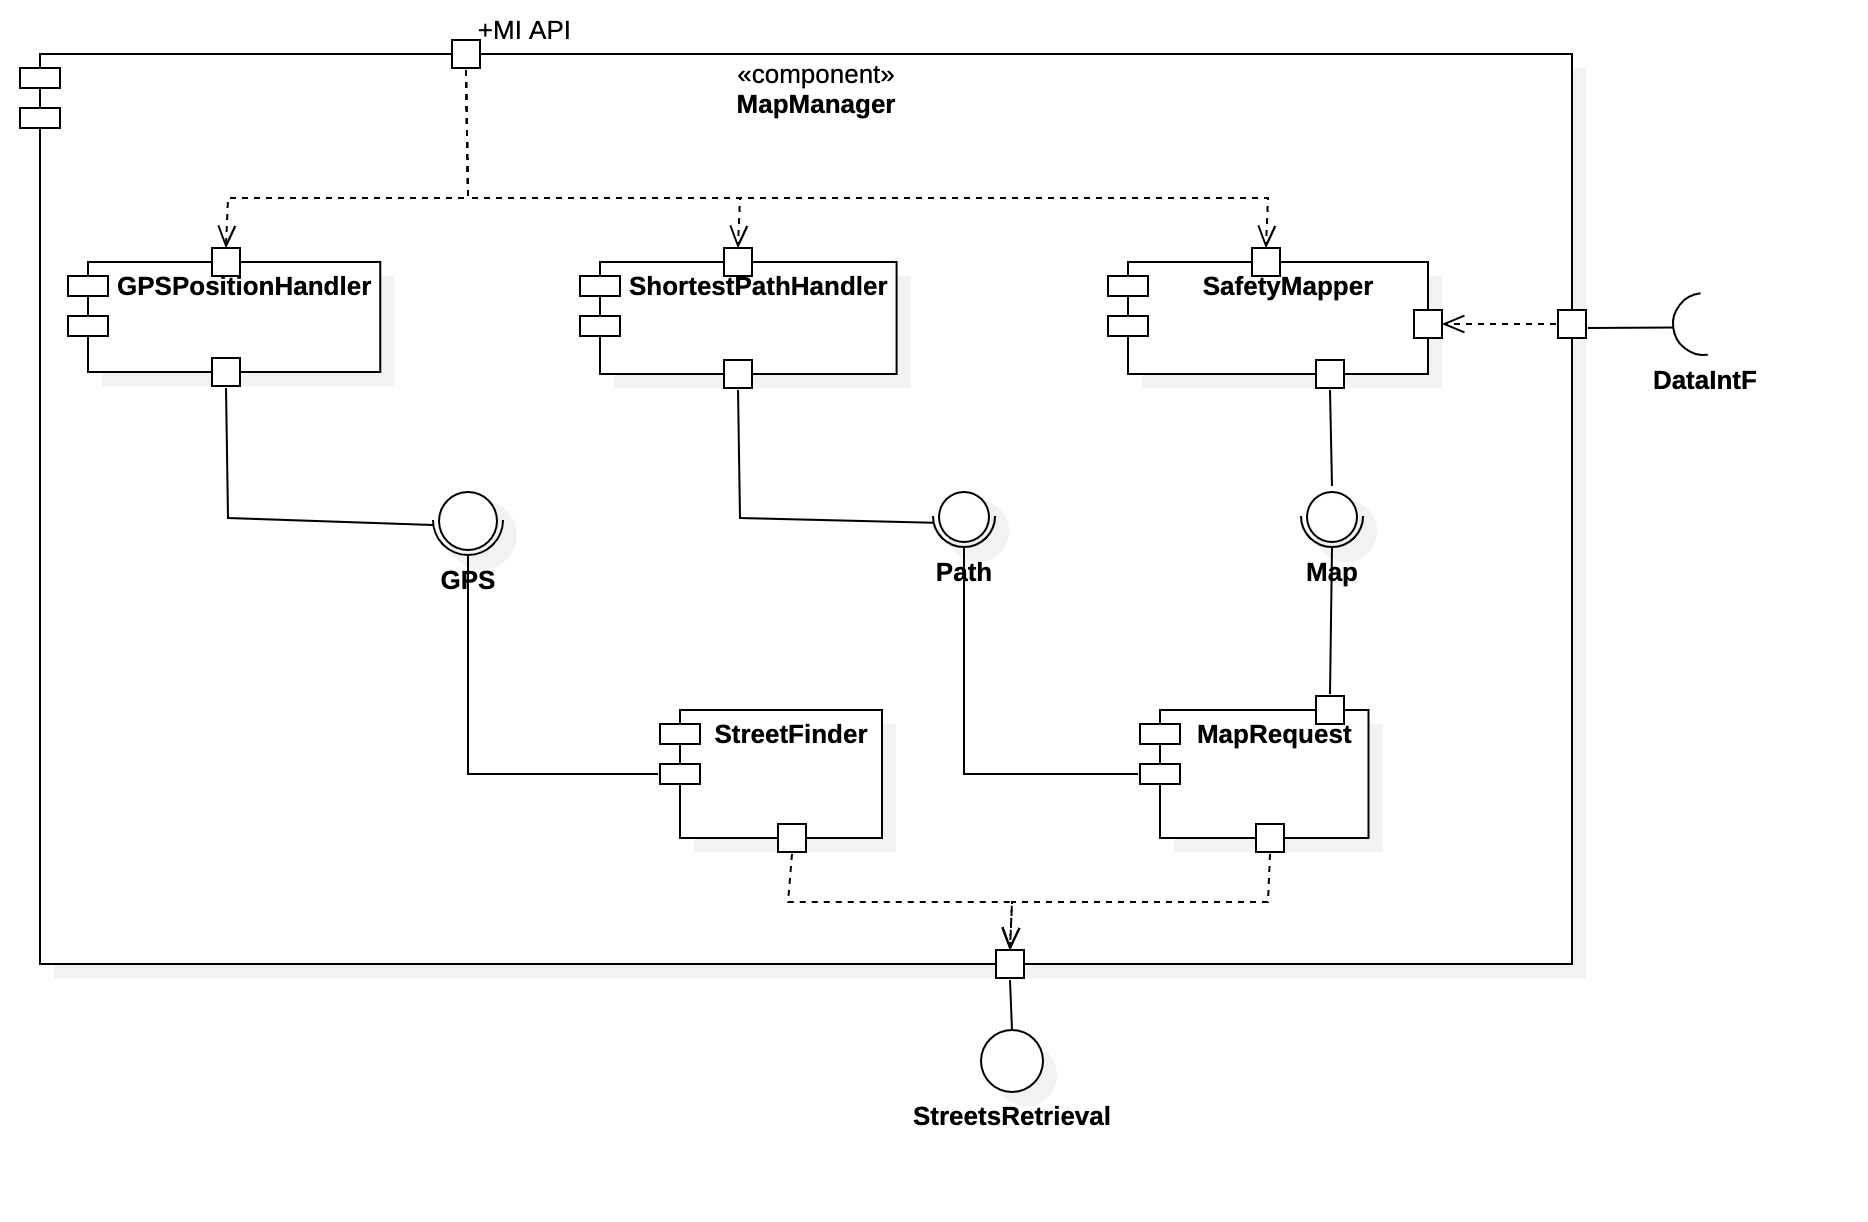
\includegraphics[scale=0.2]{/diagrams/components/mapManager.png}
				\caption{\label{fig:mapManagerComp} Map Manager Component Diagram}
			\end{figure}
		
			\begin{itemize}
				\item \textbf{SafetyMapper:} it is the component that runs the algorithms provided by the MI API once it has retrieved all the information about the safety of the streets requested by the customer. It realizes the \textbf{Map Interface} that allows to benefit of the methods that return the data of each street together with its safety in order to be displayed to the client. Hence, this is the component that receives the JSON file containing all the information needed to display a map. It parses this data and stores as it is precisely described in the data view section (\blueRef{sec:databaseView}).
			\end{itemize}
		
		\subsubsection[Safety Manager Component]{\hyperlink{toc}{Safety Manager Component}}
			\label{sec:safetyManagerComponent}
			
			The \emph{SafetyManager} (\blueAutoref{fig:safetyManagerComp}) is the component that deals with the safety computation that has to be carried out every day considering the previous thirty days in order to have the data for the safety functionality. As precisely described in the RASD \cite{RASD} we have defined a clear way to determine the safety of each street. In order to carry on this computation we have to consider this component that periodically will run its algorithms in order to update the safety.\\
			
			As we see, no interface is provided by this component, as we have just said in fact it is independent as it needs to run periodically by just retrieving the data over the notifications and accidents and update the safety of the streets.\\
			
			It is important now to describe once more how the safety update works as we can also understand how the components that compose the \emph{SafetyManager} interact in order to obtain this functionality. The system dynamically changes day by day the safety of the streets, considering the parking violations data  about the previous thirty days, thanks to two different kinds of threshold. For each street if at least one threshold is exceeded, it means that it is \textbf{unsafe} otherwise it will be considered \textbf{safe}. The thresholds are:
			
			\begin{itemize}
				\item \textbf{Intervention Threshold:} each type of violation and each accident is linked to one or more possible suggested interventions. Each type of parking violation or accident that occurs in a certain street increases the counter of the linked possible intervention for that street. If an intervention's counter in a particular street exceeds the threshold, that street will be marked as \textbf{unsafe} and that intervention will result as suggested for that particular street. In this way calculating each day for every street if a threshold for at least one intervention is exceeded allows to determine both the safety of a street and also the possible interventions to be suggested.
				
				\item \textbf{Sum Threshold:} in order to consider also the case when no accident is linked to any intervention (because of the fact we are just considering the parking violations and the accident may be caused by another reason, e.g.: the speed limit) for each street is also defined another threshold that independently from the type determines a street to be \textbf{safe} or not. There's another counter that is simply increased whenever accidents or parking violations occur in that street and thus it is simply determined as the sum of the accidents and parking violations. In this way, calculating each day for every street if the sum threshold is exceeded allows to determine the safety independently from the type of the accidents that have occurred.
			\end{itemize}
		
			Now that we know better how the safety process works we are able to describe the components that compose the \emph{SafetyManager} in order to provide this functionality:
			
			\begin{itemize}
				\item \textbf{SafetyUpdate:} it is the core component that deals with all the computation related to the calculation of the safety that we have said to happen periodically every day. In order to determine whether an interface is exceeded or not it uses the \textbf{InterventionsSafety Interface} and the \textbf{SumSafety Interface} that allow to determine for a street if one of the thresholds have exceeded. In order to access the data of the reports and the accidents the component uses the \textbf{Reports Interface} and the \textbf{Accidents Interface} to carry out the computation. Hence every day a new block of reports and accidents will be considered in the computation and the oldest one will be discarded; once the safety has been determined, the \emph{SafetyUpdate} stores the information thanks to the \textbf{Store Interface} and its functionality will be needed the next day.
				
				\item \textbf{InterventionsManager:} it is the component that realizes the \textbf{InterventionsSafety Interface} providing the methods to determine the safety of a street thanks to the thresholds of the interventions linked to the parking violations and the accidents that occurred in that street.
				
				\item \textbf{SumManager:} it is the component that realizes the \textbf{SumSafety Interface} providing the methods to determine the safety of a street thanks to its sum threshold; it counts the number of parking violations and accidents that occurred in that street.
			\end{itemize}
		
			\begin{figure}[ht]
				\centering
				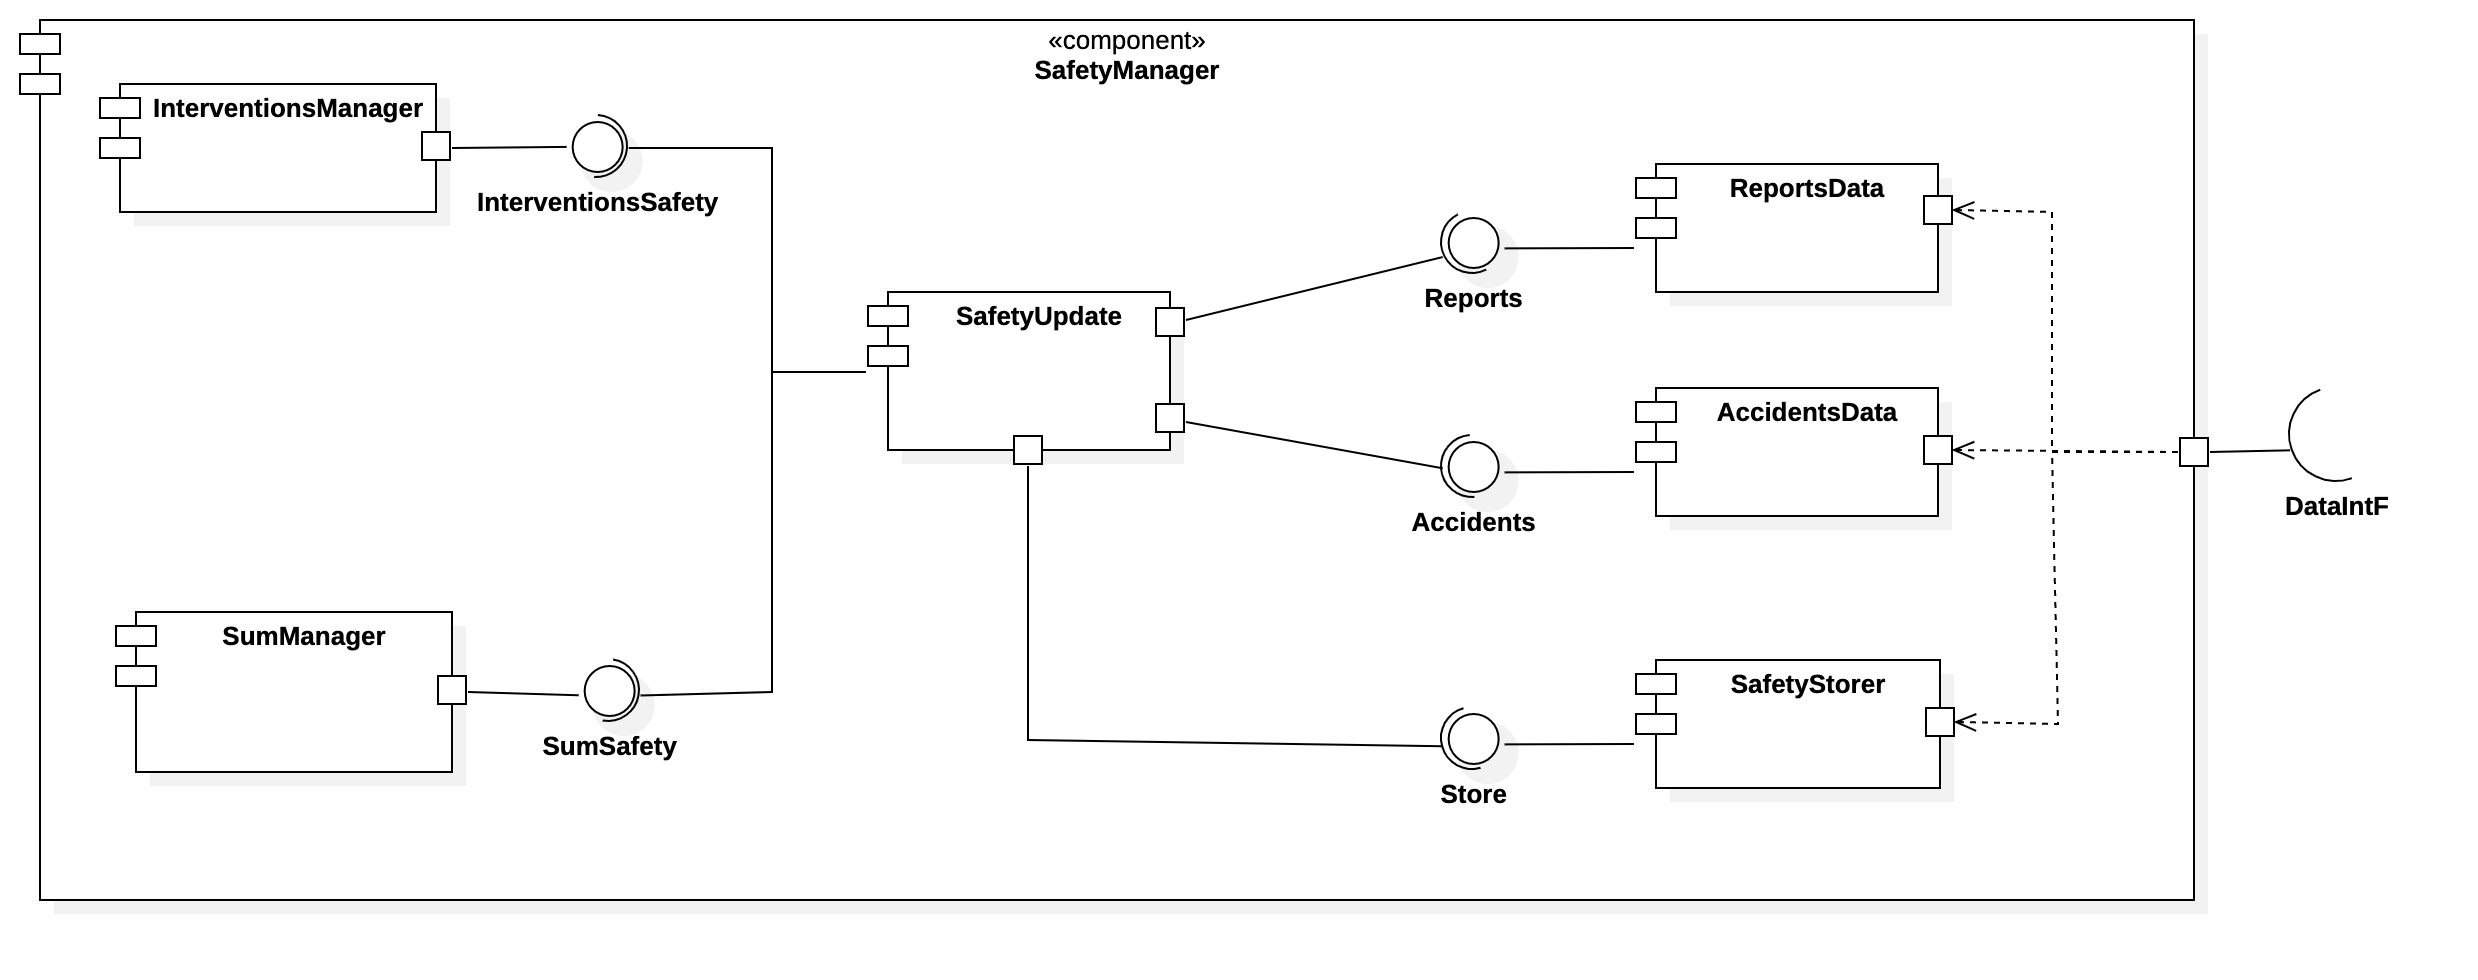
\includegraphics[scale=0.16]{/diagrams/components/safetyManager.png}
				\caption{\label{fig:safetyManagerComp} Safety Manager Component Diagram}
			\end{figure}
		
			\begin{itemize}
				\item \textbf{ReportsData:} it is the component that allows to obtain the information about the type of the parking violations that occurred in a certain street by providing the \textbf{Reports Interface} as they can be considered for the safety update.
				
				\item \textbf{AccidentsData:} it is the component that allows to obtain the information about the accidents that occurred in a certain street by providing the \textbf{Accidents Interface} as they can be considered for the safety update.
				
				\item \textbf{SafetyStorer:} it is the component that is able to store the new information about the safety of each street once it has been updated. It realizes the \textbf{Store Interface} and needs to use the methods provided by the \textbf{DataIntF Interface} in order to complete the storing action.
			\end{itemize}
		
		\subsubsection[Accidents Manager Component]{\hyperlink{toc}{Accidents Manager Component}}
			\label{sec:accidentsManagerComponent}
			
			The \emph{AccidentsManager} (\blueAutoref{fig:accidentsManagerComp}) is the component that deals just with the management of the accidents that have been stored by the authorities onto the common interface. As we see, only two components are needed: one that receives the accidents by using the methods provided by the \textbf{Authority API} and the other which stores the accidents that have been retrieved.\\
			
			The components that allow the \emph{AccidentsManager} to handle the process of receiving the accidents provided by the authorities are:
			
			\begin{itemize}
				\item \textbf{Accidents Receiver:} it is the component that uses the methods provided by the \textbf{Authority API} in order to retrieve all the accidents that each authority has published. In this way, by updating this type of data periodically we will be able to have always all the information we need to determine the safety of the streets. Once the accidents data is retrieved, this component is ready to store it in the database thanks to the \textbf{Store Interface}.
			\end{itemize}
			
			\begin{figure}[ht]
				\centering
				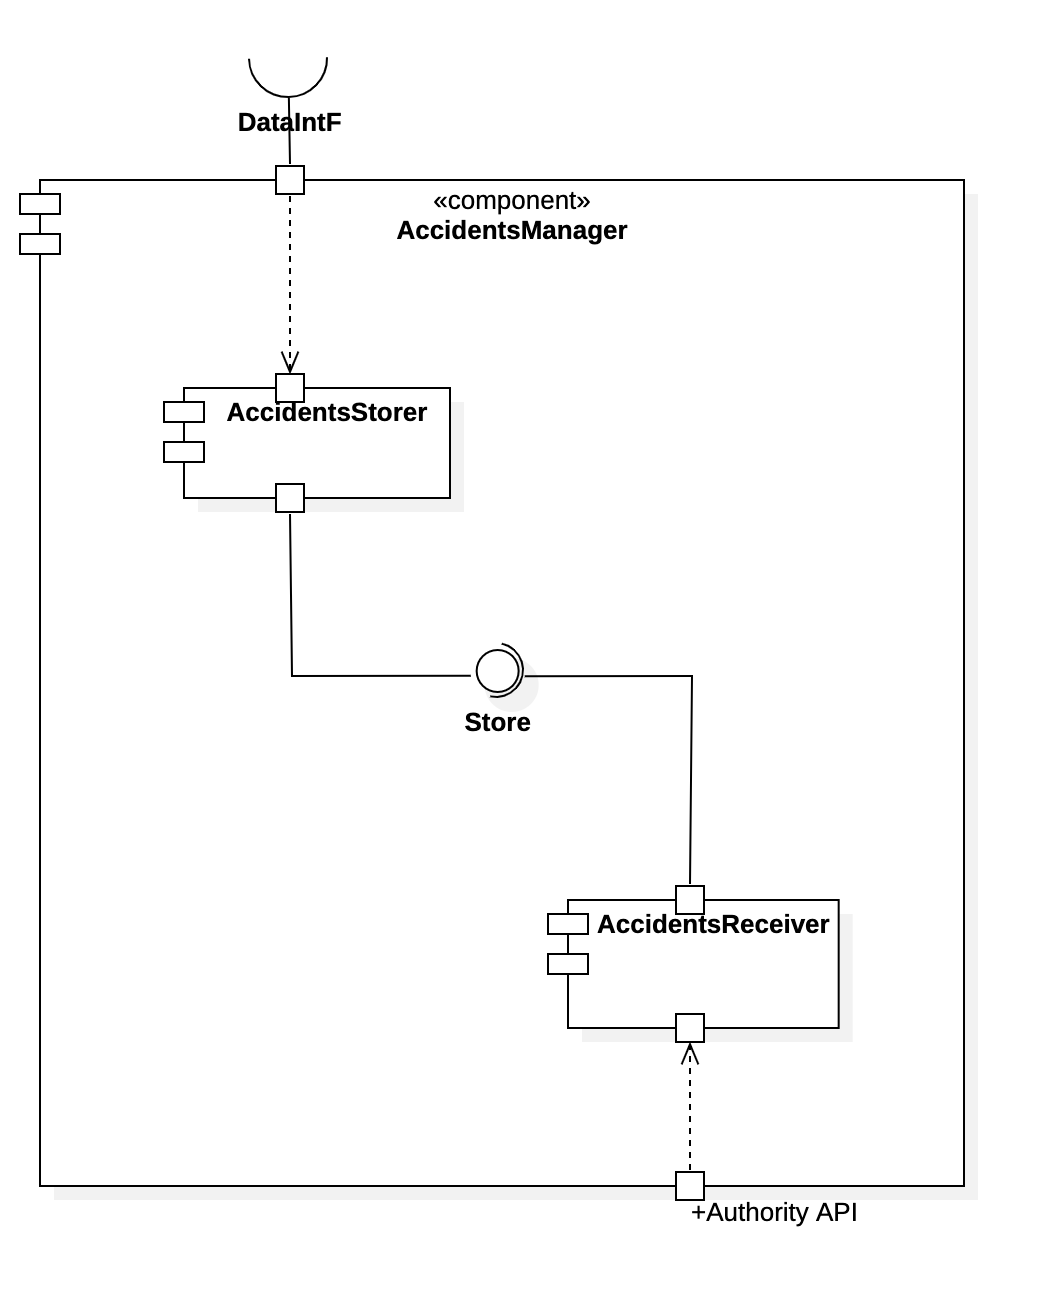
\includegraphics[scale=0.2]{/diagrams/components/accidentsManager.png}
				\caption{\label{fig:accidentsManagerComp} Accidents Manager Component Diagram}
			\end{figure}
		
			\begin{itemize}
				\item \textbf{AccidentsStorer:} it is the component that deals with the storing process of the accidents. It realizes the \textbf{Store Interface} and needs to use the methods provided by the \textbf{DataIntF Interface} in order to store the accidents in the database of the system.
			\end{itemize}
		
		\subsubsection[Data Manager Component]{\hyperlink{toc}{Data Manager Component}}
			\label{sec:dataManagerComponent}
			
			The \emph{DataManager} (\blueAutoref{fig:dataManagerComp}) is the component that deals with all the management of the data needed by the system in order to perform its functionalities. As we can see in the general diagram of the server (\blueAutoref{fig:serverComp}), almost every component needs to use the interface provided by this one.\\
			
			Hence the \emph{DataManager} realizes only the \textbf{DataIntF Interface} which provides the methods for the management of all the information and uses the methods provided by the \textbf{DBMS API} in order to perform on the database the storing or requesting actions needed.\\
			
			The components that allow the \emph{DataManager} to handle all the operations that involve the management of the data stored in the system's database are:
			
			\begin{itemize}
				\item \textbf{SafetyManager:} it is the component that provides all the methods that allow to manage the data relative to the mapping of the safety on the streets required, realizing the \textbf{DataIntF Interface}.
				
				\item \textbf{CustomersManager:} it is the component that provides all the methods that allow to manage the data relative to the customers (in particular for the access process), realizing the \textbf{DataIntF Interface}. 
				
				\item \textbf{ViolationManager:} it is the component that provides both methods that allow to manage the data relative to the notification process and the ones relative to the basic functionalities, realizing the \textbf{DatIntF Interface}.
				
				\item \textbf{InterventionsManager:} it is the component that provides all the methods that allow to manage the data relative to the interventions, realizing the \textbf{DataIntF Interface}.
				
				\item \textbf{AccidentsManager:} it is the component that provides all the methods that allow to manage the data relative to the accidents, realizing the \textbf{DataIntF Interface}.
			\end{itemize}
		
			\begin{figure}[ht]
				\centering
				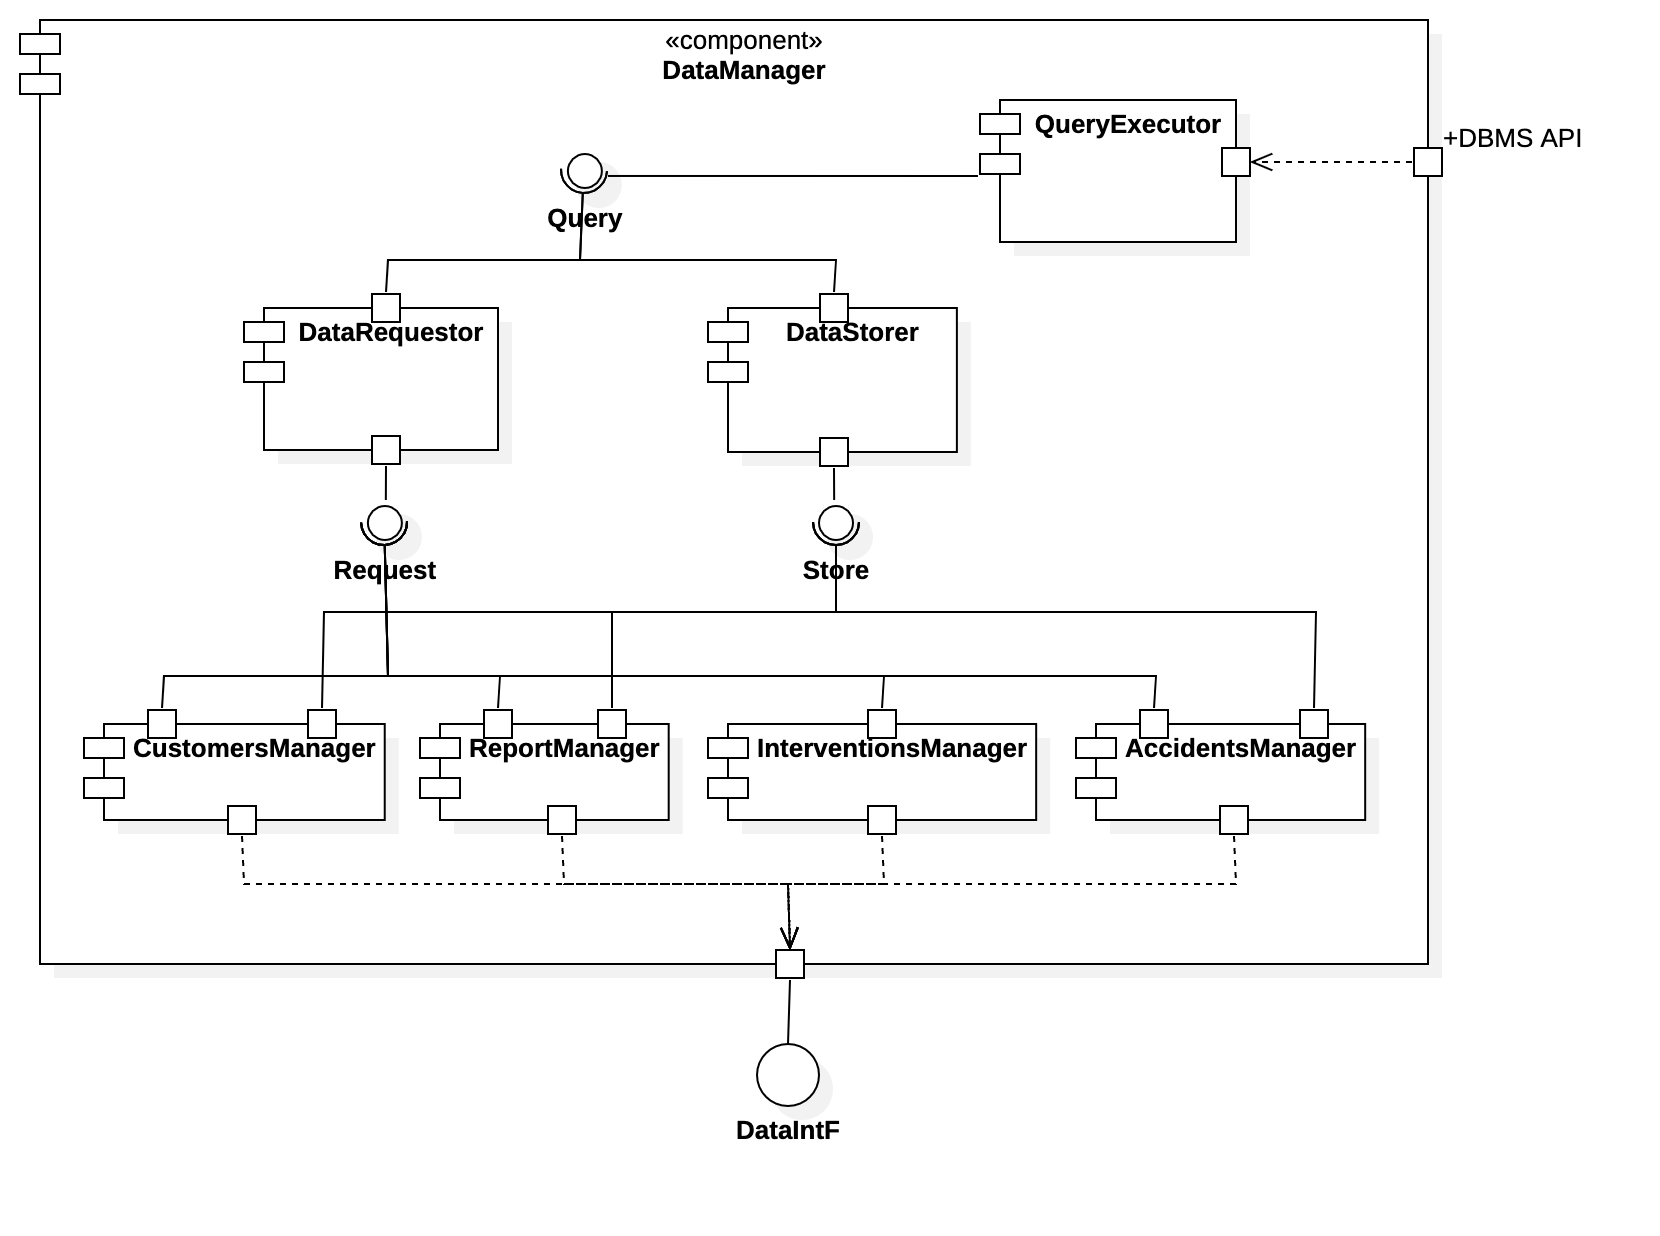
\includegraphics[scale=0.2]{/diagrams/components/dataManager.png}
				\caption{\label{fig:dataManagerComp} Data Manager Component Diagram}
			\end{figure}
		
			\begin{itemize}
				\item \textbf{DataRequestor:} it is the component that allows to build a query that will obtain as a result the information required by one of the managers previously described. It realizes the \textbf{Request Interface} and needs to use the \textbf{Query Interface} in order to execute the query that has been built.
				
				\item \textbf{DataStorer:} it is the component that allows to build a query that will store in the database the data provided by the component that invokes its methods. It realizes the \textbf{Store Interface} and needs to use the \textbf{Query Interface} in order to execute the query that has been built.
				
				\item \textbf{QueryExecutor:} it is the component that finally executes the query received either from the \emph{DataRequestor} or the \emph{DataStorer}. It realizes the \textbf{Query Interface} and needs to use the methods provided by the \textbf{DBMS API} in order to manage all the data stored inside the database of the system.
			\end{itemize}
		
		\subsubsection[Web Server Component]{\hyperlink{toc}{Web Server Component}}
			\label{sec:webServerComponent}
			
			The \emph{WebServer} (\blueAutoref{fig:webServerComp}) is an independent component, out of the server, that deals with the interaction between the web app and the business logic of the system. It realizes the \textbf{WebAppInterface} in order to provide the endpoint for the authorities to access SafeStreet with the web application displayed on their browser. It needs to use the methods provided by the \textbf{WebInterface} in order to establish the interaction between the authorities and the system.\\
			
			The components that allow the \emph{WebServer} to handle the interaction process between the requests coming from the web app and the business logic are:
			
			\begin{itemize}
				\item \textbf{Presentation:} it is the component that deals with the graphical interface that is needed to provide the authorities the access to the system. It realizes the \textbf{WebAppInterface} as it defines all the methods and scripts the browser will use to display the information. In order to manage the interaction, it handles the actions performed by the authority with the \textbf{Commands Interface} and sends the requests to the system as they can be processed thanks to the \textbf{Requests Interface}.
			\end{itemize}
			
				\begin{figure}[ht]
					\centering
					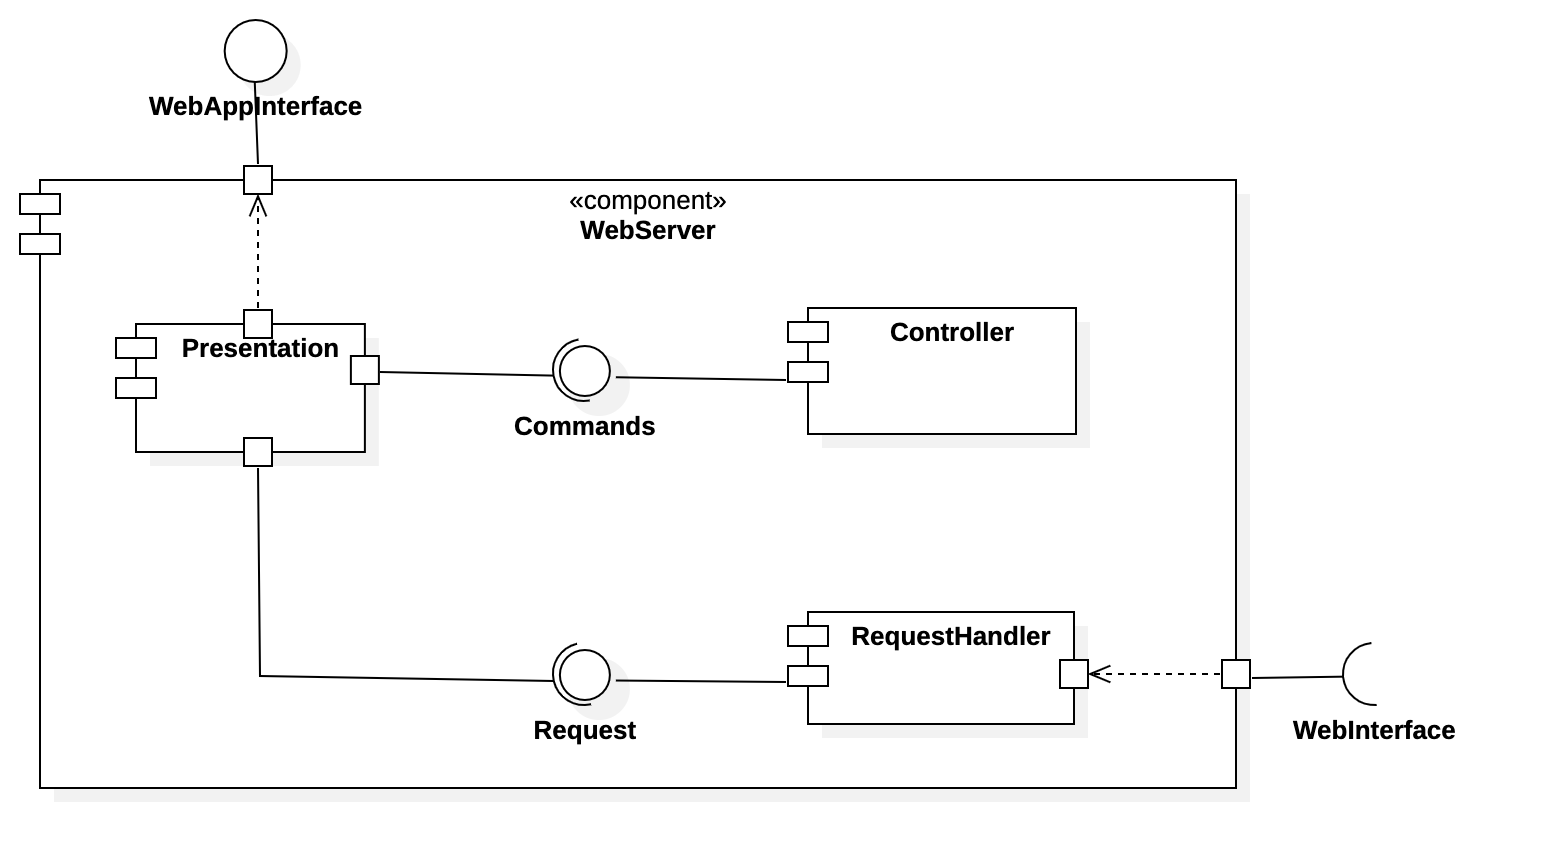
\includegraphics[scale=0.2]{/diagrams/components/webServer.png}
					\caption{\label{fig:webServerComp} Web Server Component Diagram}
				\end{figure}
		
			\begin{itemize}
				\item \textbf{Controller:} it is the component that deals with the logic needed to handle the actions performed by the authority. By providing the \textbf{Commands Interface} it allows to manage the flow of the web application displayed on the browser of the authority.
				
				\item \textbf{RequestHandler:} it is the component that deals with all the requests coming from the web application. Thanks to the \textbf{Request Interface} realized, it is able to process the incoming request and send it to the business logic with the methods of the \textbf{WebInterface} as the functionality required will be displayed in the web application.
			\end{itemize}
		
		\subsubsection[User App Component]{\hyperlink{toc}{User App Component}}
			\label{sec:userAppComponent}
			
			The \emph{UserApp} (\blueAutoref{fig:userAppComp}) is the other independent component that will be installed on the device of the users in order to provide the interaction with the system. Differently from the \emph{WebServer} this is already the component that will manage the actions performed by the user as it represents the mobile software application. For this reason it only needs to use the methods provided by the \textbf{MobileAppInterface} to send the requests to the system as they can be processed.\\
			
			The components that allow the \emph{UserApp} to handle the interaction process between the requests coming from the mobile app and the business logic are:
			
			\begin{itemize}
				\item \textbf{Presentation:} it is the component that deals with the graphical interface that is needed to provide the users the access to the system. As we have just said, the realization of this component is the interface that allows the user to interact with the system; in order to do so it needs to use the methods provided by the \textbf{Commands Interface} and the \textbf{Request Interface}.
			\end{itemize}
			
			\begin{figure}[ht]
				\centering
				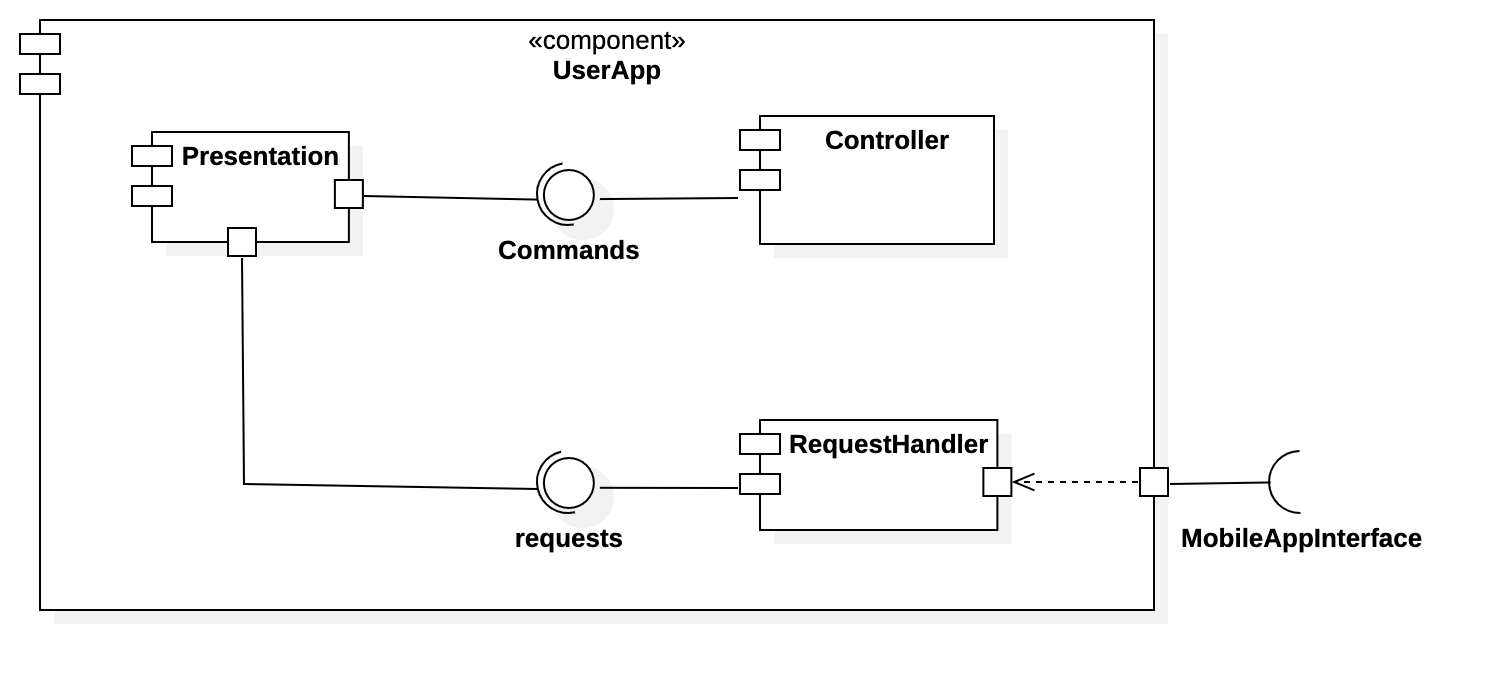
\includegraphics[scale=0.2]{/diagrams/components/userApp.png}
				\caption{\label{fig:userAppComp} User App Component Diagram}
			\end{figure}
		
			\begin{itemize}
				\item \textbf{Controller:} it is the component that deals with the logic needed to handle the actions performed by the authority. By providing the \textbf{Commands Interface} it allows to manage the flow of the mobile application displayed on the device of the user.
				
				\item \textbf{RequestHandler:} it is the component that deals with all the requests coming from the mobile application. Thanks to the \textbf{Request Interface} realized, it is able to process the incoming request and send it to the business logic with the methods of the \textbf{MobileAppInterface} as the functionality required will be displayed in the application.
			\end{itemize}
			
	\subsection[Database View]{\hyperlink{toc}{Database View}}
		\label{sec:databaseView}
		
		Before giving the description of how the components now presented will be deployed in our system, it is also important to define a model that allows to manage the huge amount of data we expect to deal with. As we will also motivate later, in section \blueRef{sec:selectedArchitecturalStylesAndPatterns}, we decided to use a relational approach to store the information we need to manage. In order to do so we decided to use a class diagram model rather than an entity-relationship one as we could give a continuous representation of what we already presented in the RASD \cite{RASD}. The class diagram in theS next page, in fact, has been updated with more detailed considerations that we are now able to consider, being at the design level.\\
		
		As we can see in the picture (\blueAutoref{fig:classDiagramModel}), some classes and relations have been updated, in particular for what concerns the maps issues and the safety ones. In particular:
		
		\begin{itemize}
			\item The classes that we are going to use to store the position issues have been updated. We removed the \textbf{Position} class as it is not relevant anymore while we added the \textbf{Cross} class that is important for the transportation of the data relative to a map to be highlighted. The \textbf{Path} class has also been updated to consider a possible way to store the information relative to a path provided by the MI. The \textbf{Street} and \textbf{City} classes are still considered as we have said that we need to store in our system their information in order to deal with the functionalities the system has to provide.
			
			\item The most important update is the \textbf{Map} class. This class is the result of the invocation of the methods that deal with the \emph{UnsafeStreets} functionality. What happens, in fact, when a request of this type arrives to the business logic is: first retrieve in the database all the requested streets and their safety, second, provide them to the methods of the MI that will return the JSON file containing all the relevant information for a map to be displayed. Thanks to this class, we will easily parse the file and store its values in the class attributes.
			
			\item The \textbf{Safety} class has also been removed as it was used in the initial class diagram to define more precisely which were the relations that allowed to determine its value for the streets stored in the system. We decided now to simplify the safety considerations, even to reduce the complexity of the algorithms that will determine it, by storing in each street a value that is \emph{true} if the street is safe, otherwise \emph{false}.		
		\end{itemize}
		
		\newpage
		
		\begin{figure}[ht!bp]
			\centering
			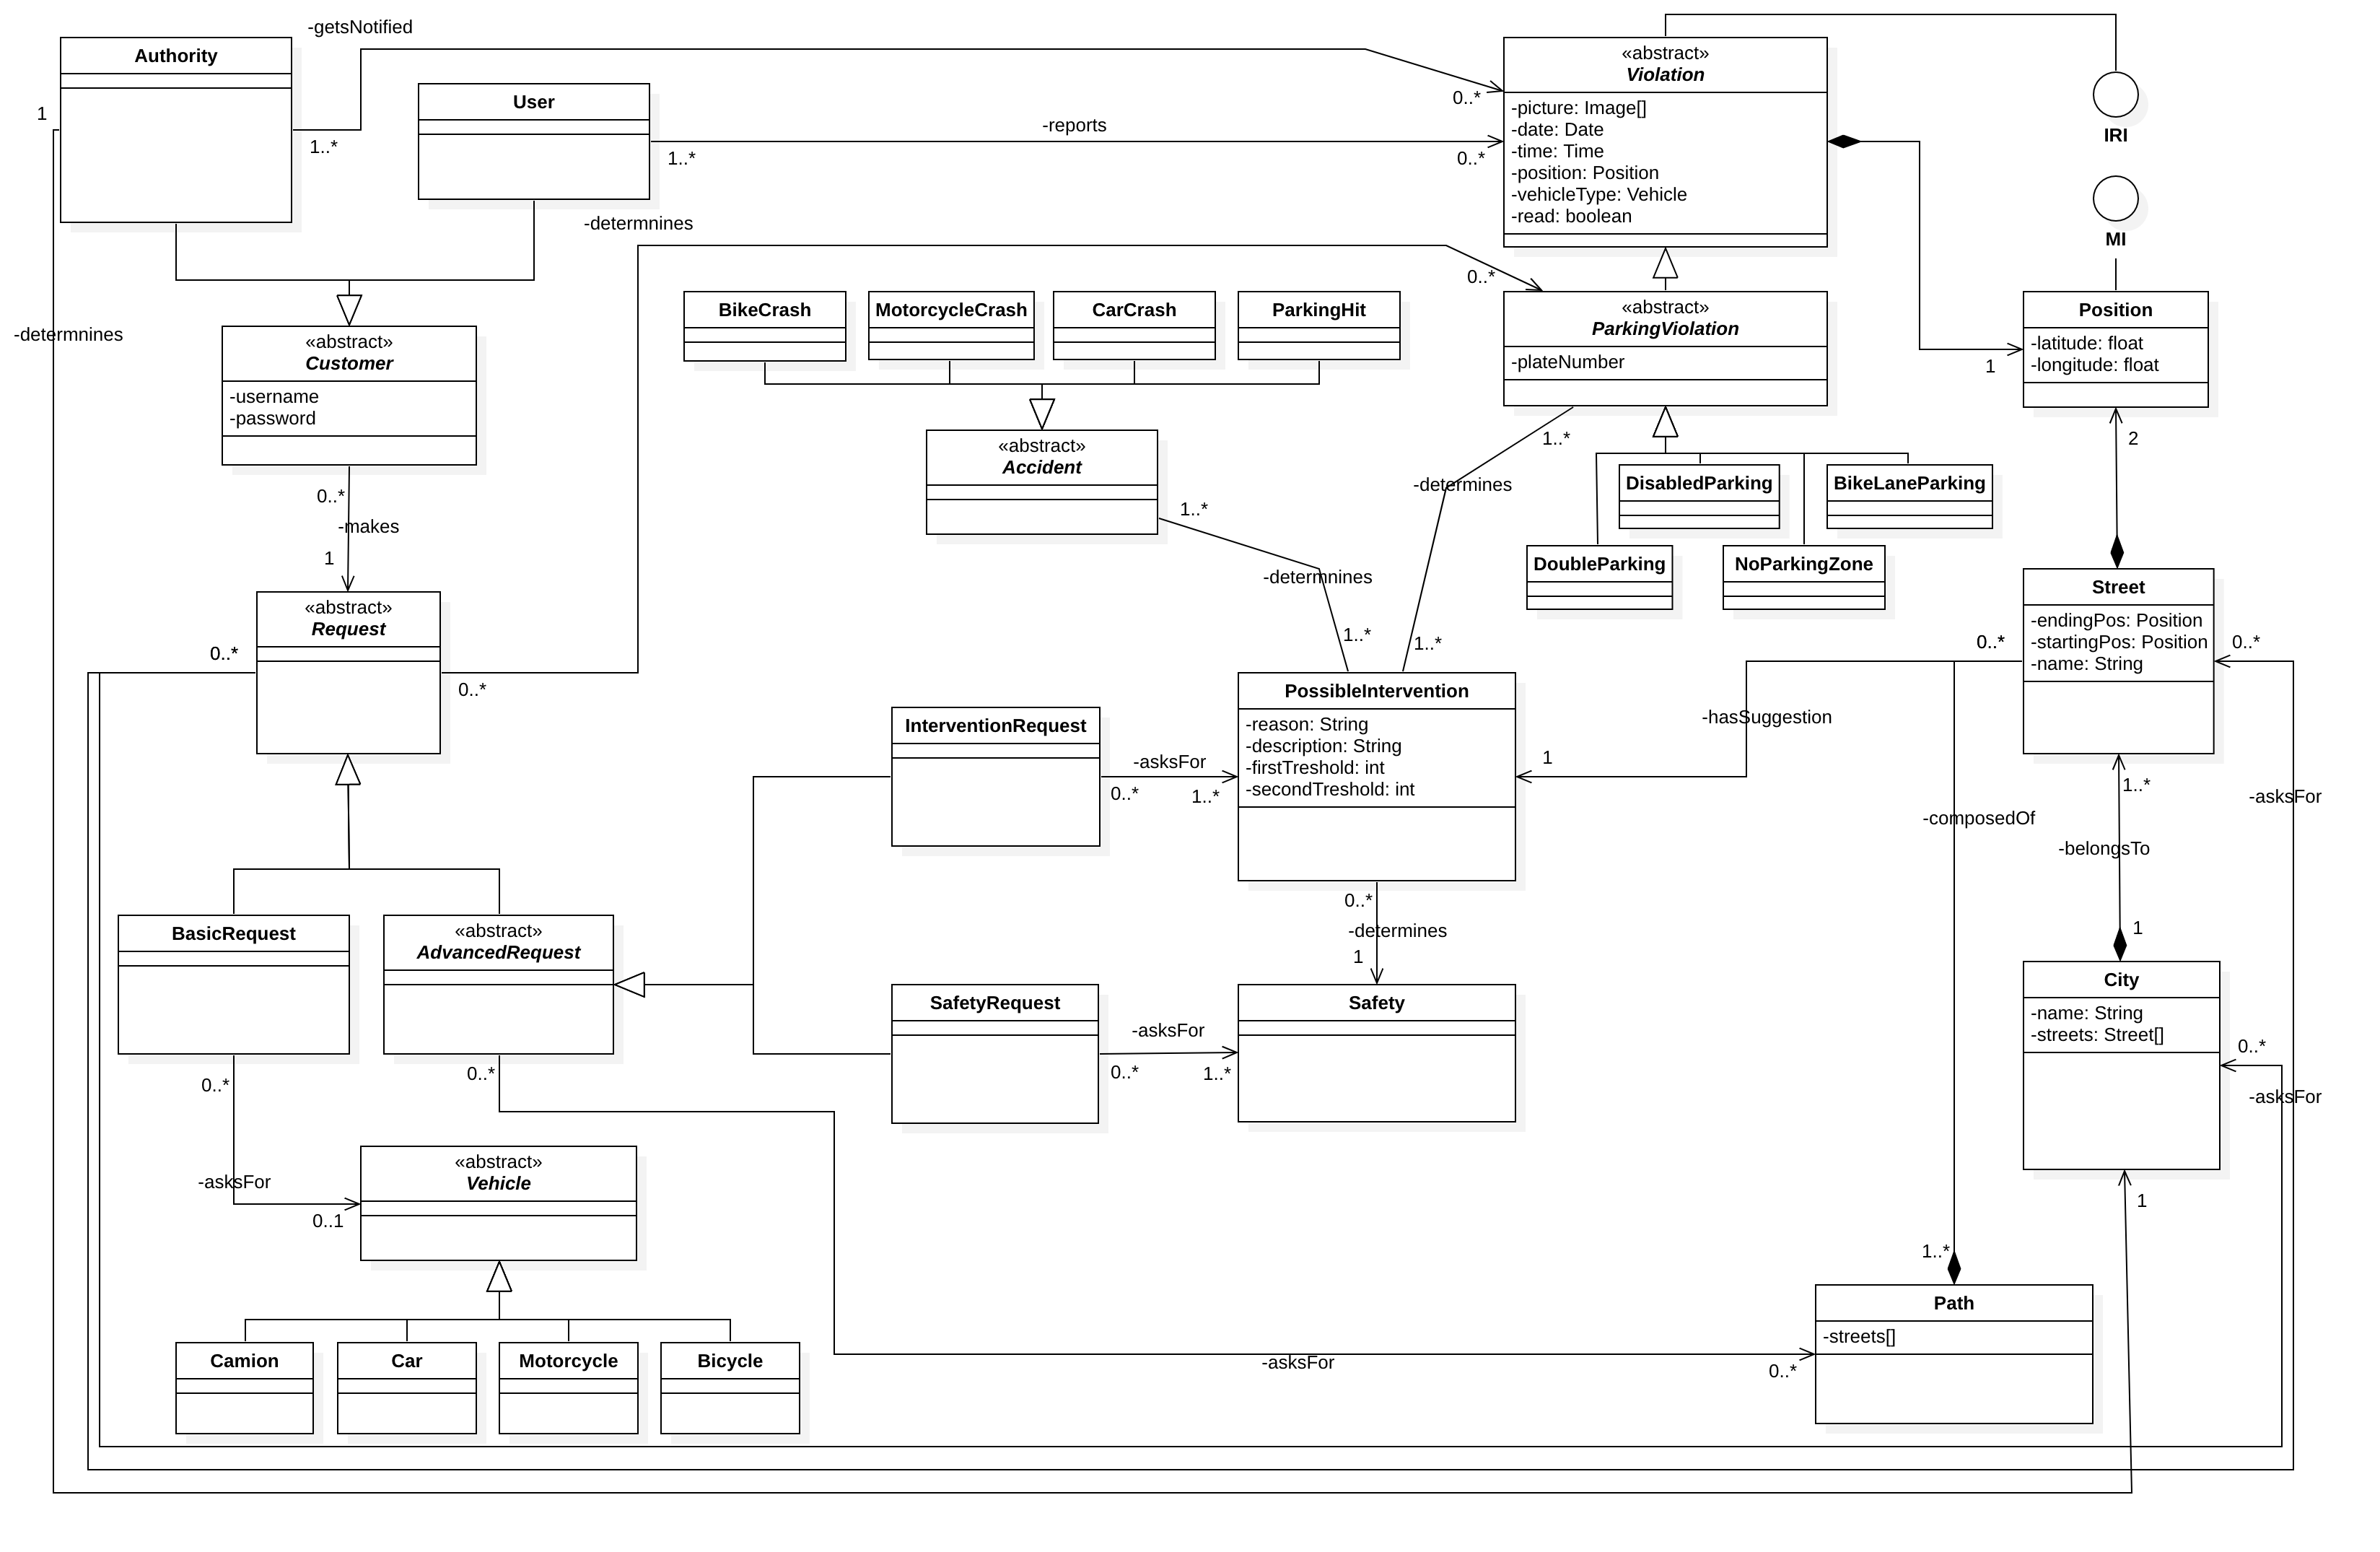
\includegraphics[scale=0.175, angle=90]{/diagrams/classDiagramModel.png}
			\caption{\label{fig:classDiagramModel} Class Diagram Model}
		\end{figure}
	
		\FloatBarrier
		
		To conclude with this section that aims to provide an overview of which type of data will flow inside our system, we want to give a practical example of how the objects of the \textbf{Map} class will be instantiated once we receive as a result the JSON file from the MI. What we want to achieve is a one to one correspondence between the file and the class as we can store all the information with just one method invocation of some parsing library. Hence, what we aim to is something like presented in the following picture:
		
		\begin{figure}[h!]
			\centering
			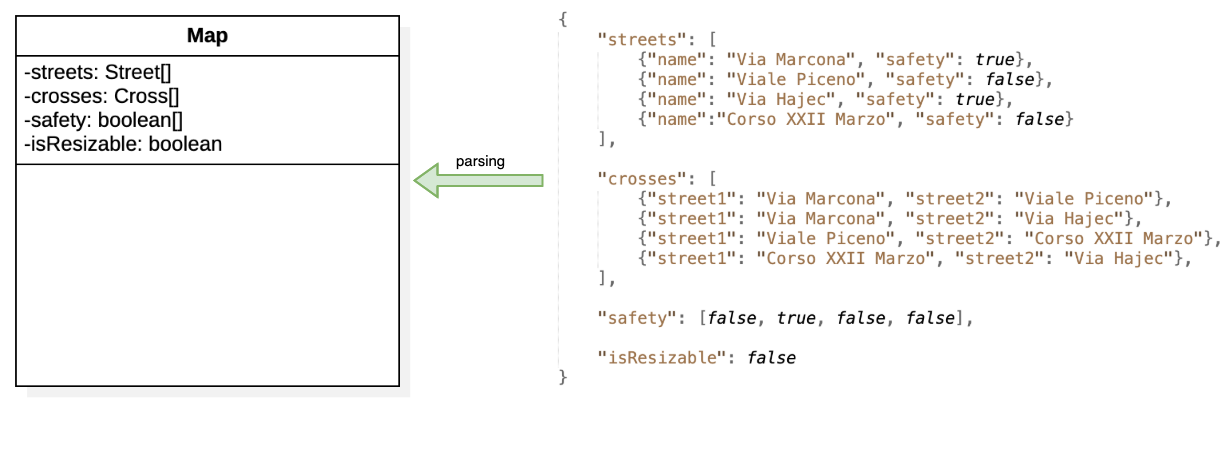
\includegraphics[scale=0.3]{miscellaneous/jsonMapping.png}
			\caption{\label{fig:jsonMapping} Map-Class and Json-File Correspondence}
		\end{figure}
	
		Thanks to this information we will be able to use the map objects and display for our clients the safety they are requiring, in fact:
		
		\begin{itemize}
			\item The \emph{streets} are the ones that have to be displayed
			\item The \emph{crosses} establish how the streets are disposed
			\item The \emph{safety} array specifies the safety of the crosses
			\item The \emph{isResazible} attribute specifies if the map is resizable or not
		\end{itemize}
	
		\newpage
	
	\subsection[Deployment View]{\hyperlink{toc}{Deployment View}}
		\label{sec:deploymentView}

		As we have seen in the overview (\blueRef{sec:overview}) and component view (\blueRef{sec:componentView}) sections, we have designed a system that needs to interact with many agents. In order to define a crowd-sourced application where a lot of information needs to be managed as it can be used to provide different services, we decided to use a \textbf{client-server} architectural approach. As we may have guessed in the high-level component diagram of \blueAutoref{fig:highLevelComp} the business logic is represented by the server component while the clients are designed with two different technologies in order to have the best application software to make the customers interact with the system.\\
		
		The client-side system is composed of:
		
		\begin{itemize}
			\item \textbf{Mobile Application:} for the users
			\item \textbf{Web Application:} for the authorities
		\end{itemize}
			
		Hence, to make this decision possible we need to consider a web server that will manage all the interactions between the web application and the internal system, while we can make directly interface the mobile application with the internal system thanks to the software application installed on the devices of the users.\\
		
		To accomplish the considerations just presented we decided to design the \textbf{client-server} paradigm with a \textbf{four-tier architecture} in order to have a clear separation between the clients and the servers that manage them; the decoupling of the database shown in the composition diagram (\blueAutoref{fig:compositionDiagram}) enforces once more this decision. All the communications between the system and the customers (both users and authorities) are handled via HTTP messages in a RESTful way (HTTPS is shown in the diagram for obvious security reasons). All the considerations just reported about some architectural and communication choices will be clearly precised in the devoted section (\blueRef{sec:selectedArchitecturalStylesAndPatterns}).\\
		
		Let's focus now on the illustration of the four-tier architecture as we can understand how the components that we have previously described are mapped with the tiers of the system. Then, in the next section we first illustrate the decision tree we used while designing the system as we can later give the complete description of the deployment.\\
		
		The following picture (\blueAutoref{fig:fourTierArchitecture}) illustrates the tiers of the system needed in order to deploy the components identified in the previous section. 
		
		\vspace{0.3cm}
		
		\begin{figure}[h!]
			\centering
			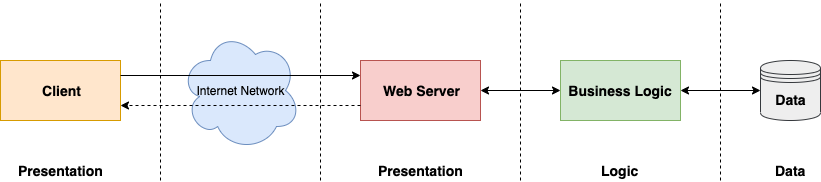
\includegraphics[scale=0.4]{architecture/fourTierArchitecture.png}
			\caption{\label{fig:fourTierArchitecture} Four Tier Architecture Diagram}
		\end{figure}
		
		\paragraph{Components Mapping} Now that we know which are the tiers and which are the components, we are able to map them together as we can clearly understand how the design is structured before starting with the deployment diagram.
		
		\begin{itemize}
			\item \textbf{Client:} are the components that allow the interaction of the customers with the system in order to benefit of its functionalities.
			
				\begin{itemize}
					\item AuthorityWebApp
					\item UserApp
				\end{itemize}
			
			\item \textbf{Web Server:} it is the layer that allows the interaction between the web application used by the authorities and the system.
			
				\begin{itemize}
					\item WebServer
				\end{itemize}
			
			\item \textbf{Business Logic:} is composed of all the components that allow the computation needed to provide the functionalities of SafeStreets. Hence it is made of all the components inside the server one that are:
			
				\begin{itemize}
					\item ClientHandler
					\item AccessManager
					\item QueryManager
					\item ReportManager
					\item MapManager
					\item SafetyManager
					\item AccidentsManager
					\item DataManager
				\end{itemize}
			
			\item \textbf{Data:} is the layer that deals with the management of all the data needed by the system in order to provide its services.
			
				\begin{itemize}
					\item DBMS
				\end{itemize}
		\end{itemize}
	
		The diagram of next page (\blueAutoref{fig:coloredComponentDiagram}) provides a graphical illustration of what we have just said by coloring the corresponding layer with the same color of the components highlighted in the general component diagram already seen.
		
		\newpage
		
		\begin{figure}[htbp]
			\centering
			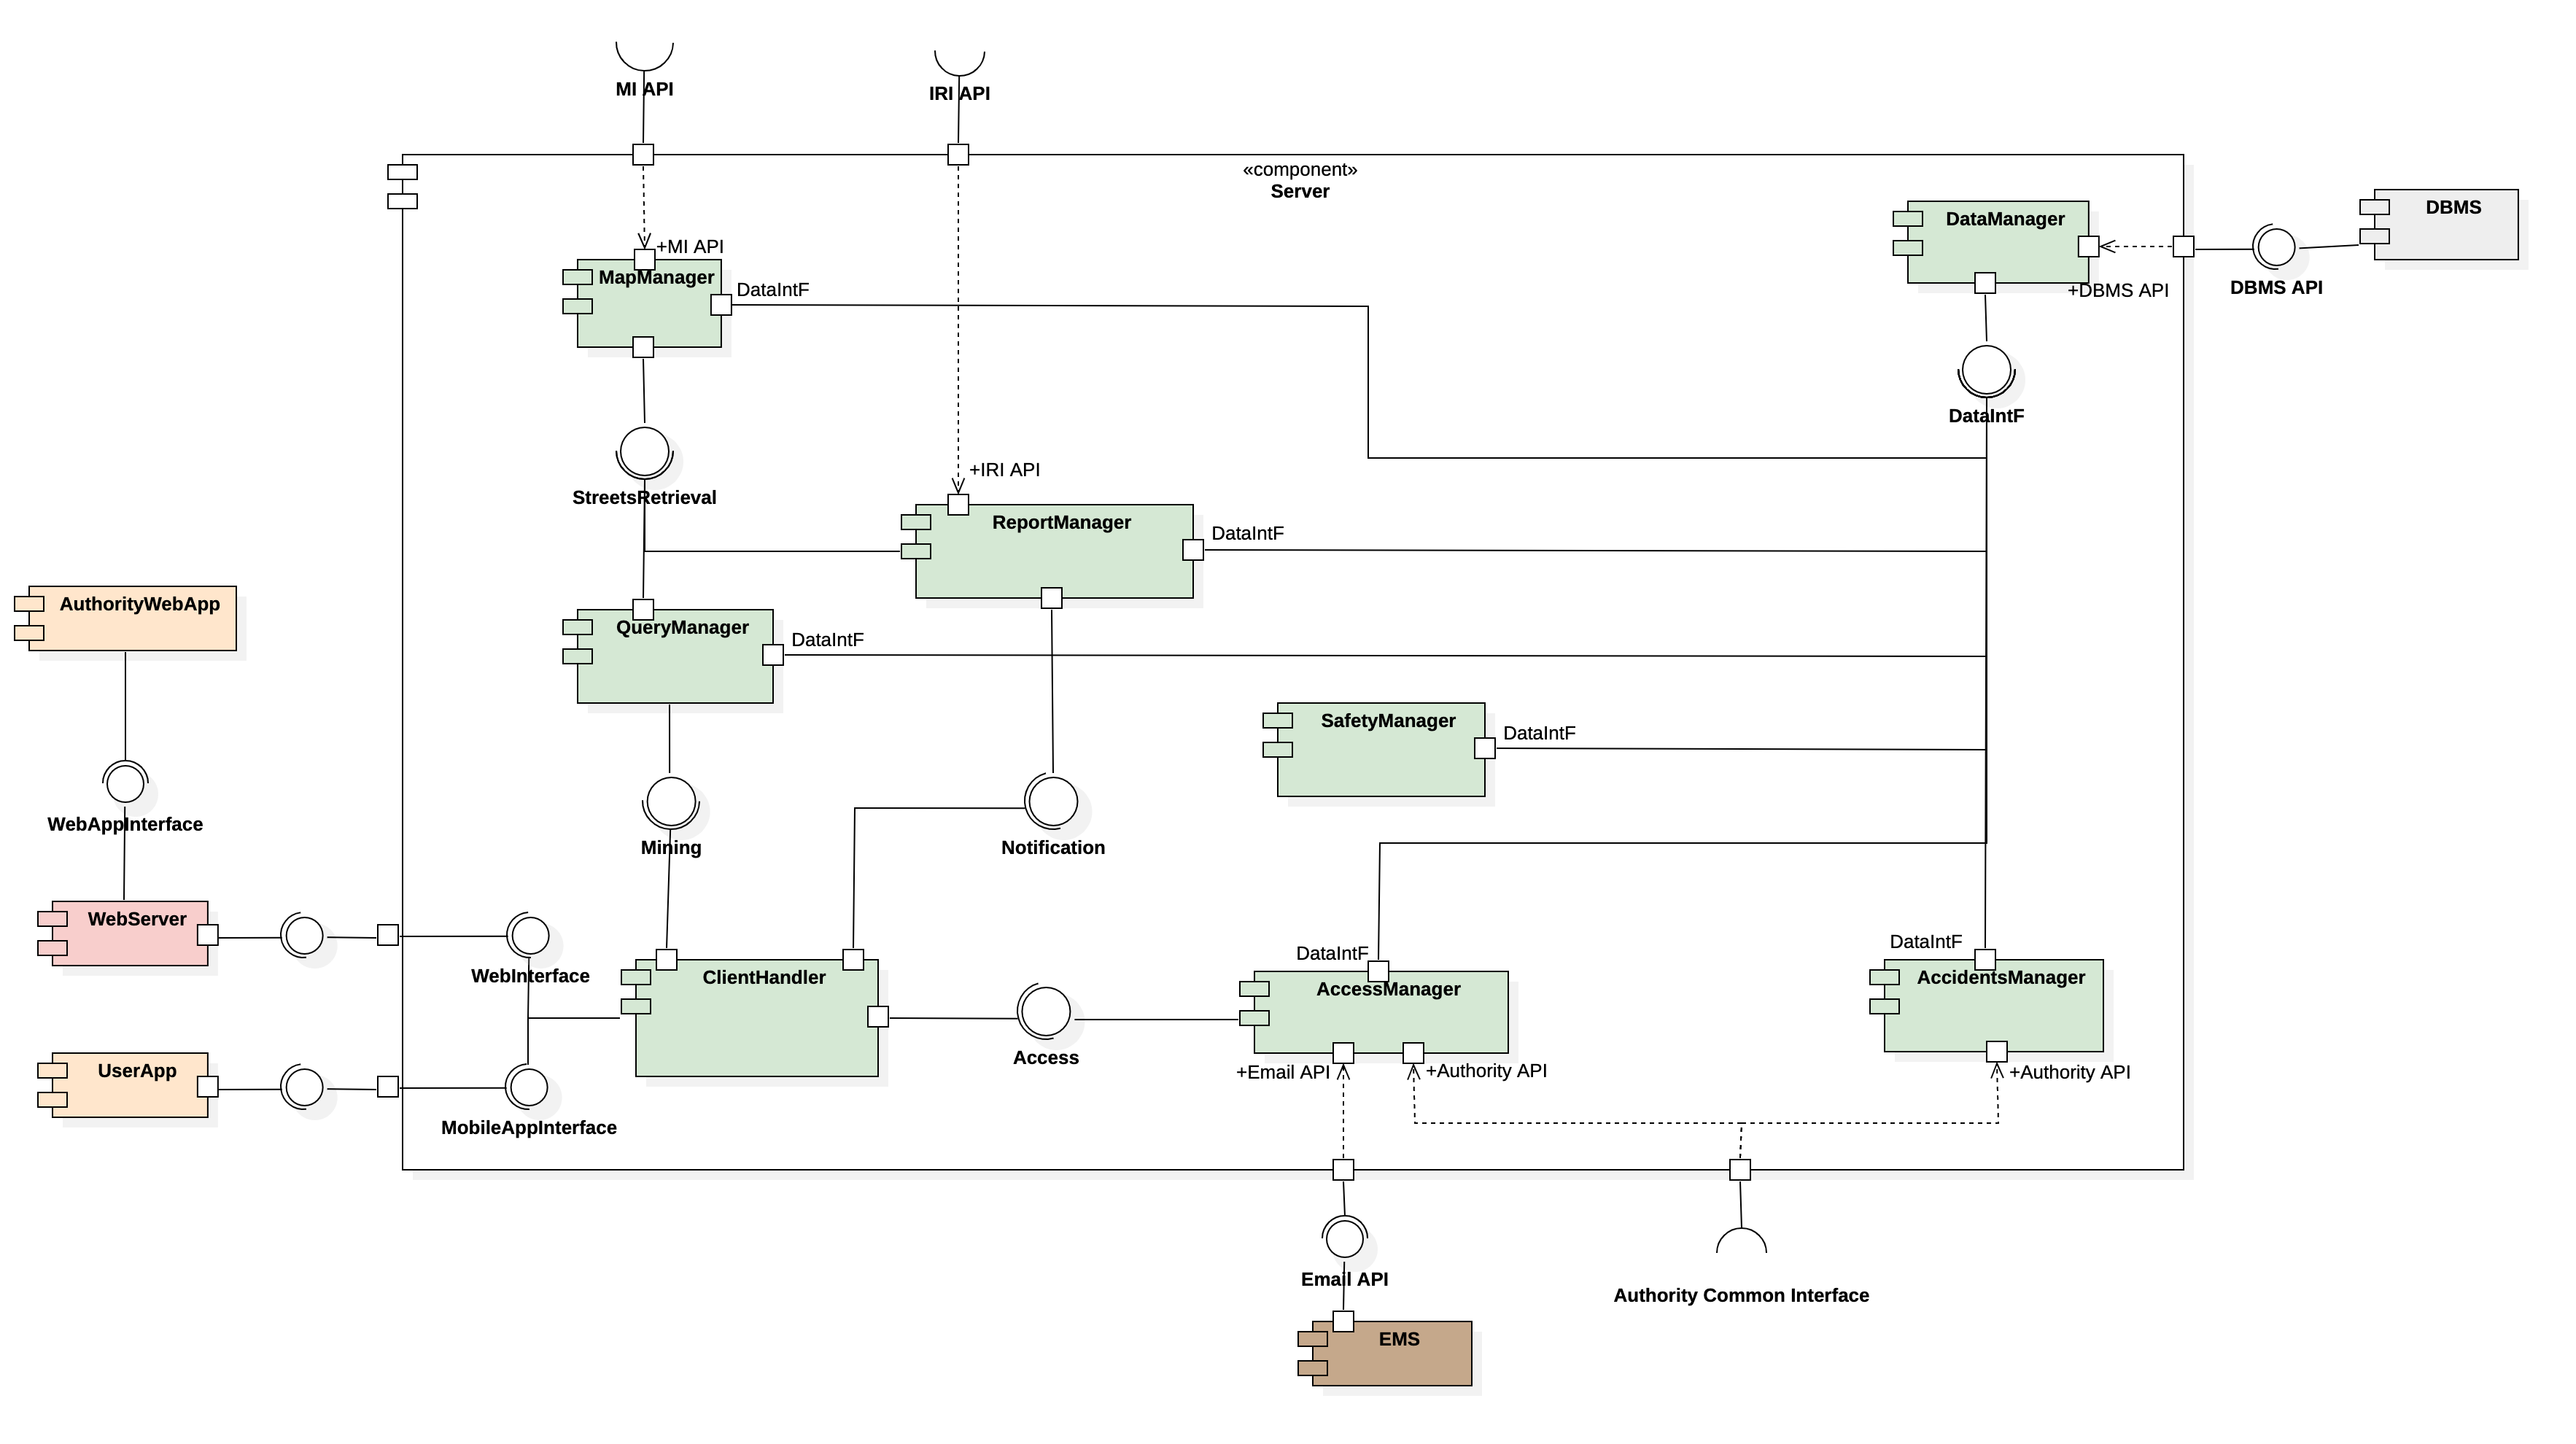
\includegraphics[scale=0.16, angle=90]{architecture/coloredComponentDiagram.png}
			\caption{\label{fig:coloredComponentDiagram} Components Mapping Diagram}
		\end{figure}
	
		\FloatBarrier
	
		\subsubsection[Decision Tree]{\hyperlink{toc}{Decision Tree}}
			\label{sec:decisionTree}
			
			Now that we have established how our system is going to be deployed at the highest level possible, before providing the most detailed deployment diagram we present the decision tree we developed while defining the design process as we can justify the diagram of the next section. As we can see in the picture (\blueAutoref{fig:decisionTree}) we started with a \textbf{client-server} decision and then refined it with further more detailed decisions.
			
			\begin{figure}[h!]
				\centering
				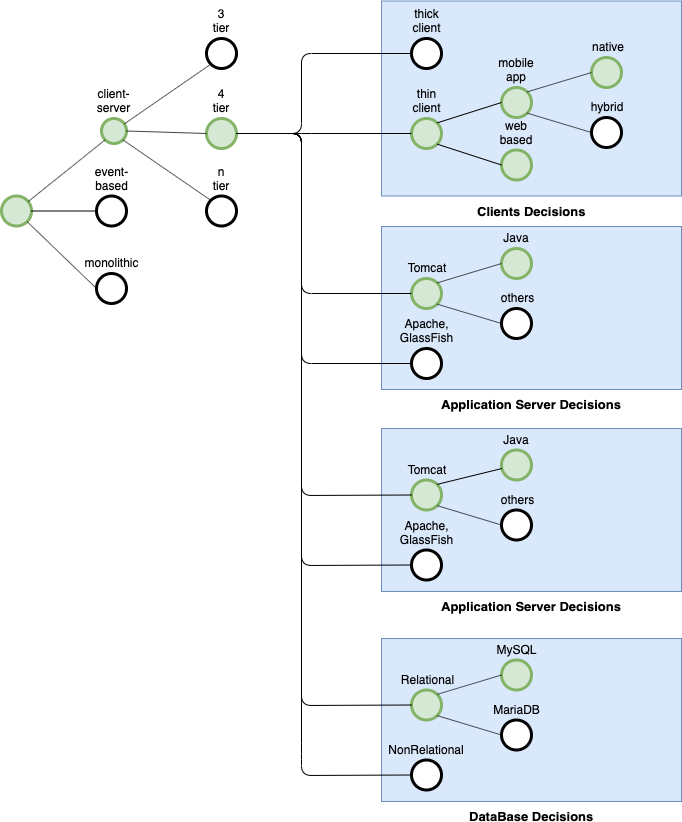
\includegraphics[scale=0.45]{miscellaneous/decisionTree}
				\caption{\label{fig:decisionTree} Decision Tree}
			\end{figure}
			
		\subsubsection[Deployment Diagram]{\hyperlink{toc}{Deployment Diagram}}
			\label{sec:deploymentDiagram}
			
			In the diagram of the following page (\blueAutoref{fig:deploymentDiagram}) we illustrate a precise description of how and where the components identified are deployed. We still use the colors related to the components now for the nodes that involve them.\\
			
			The communication is presented only between the nodes and not for the components as we already have a precise description of their interfaces that realize the interaction in the component view section (\blueRef{sec:componentView}). The \textbf{HTTPS} and \textbf{TCP/IP} protocols are used to connect respectively: a connection to a REST API or to a service providing system.\\
			
			All the motivations for the architectural styles and patterns but also the implementation choices that we can see in the picture will be clearly motivated in the devoted section (\blueRef{sec:selectedArchitecturalStylesAndPatterns}). 
						
			\begin{figure}[hbtp]
				\centering
				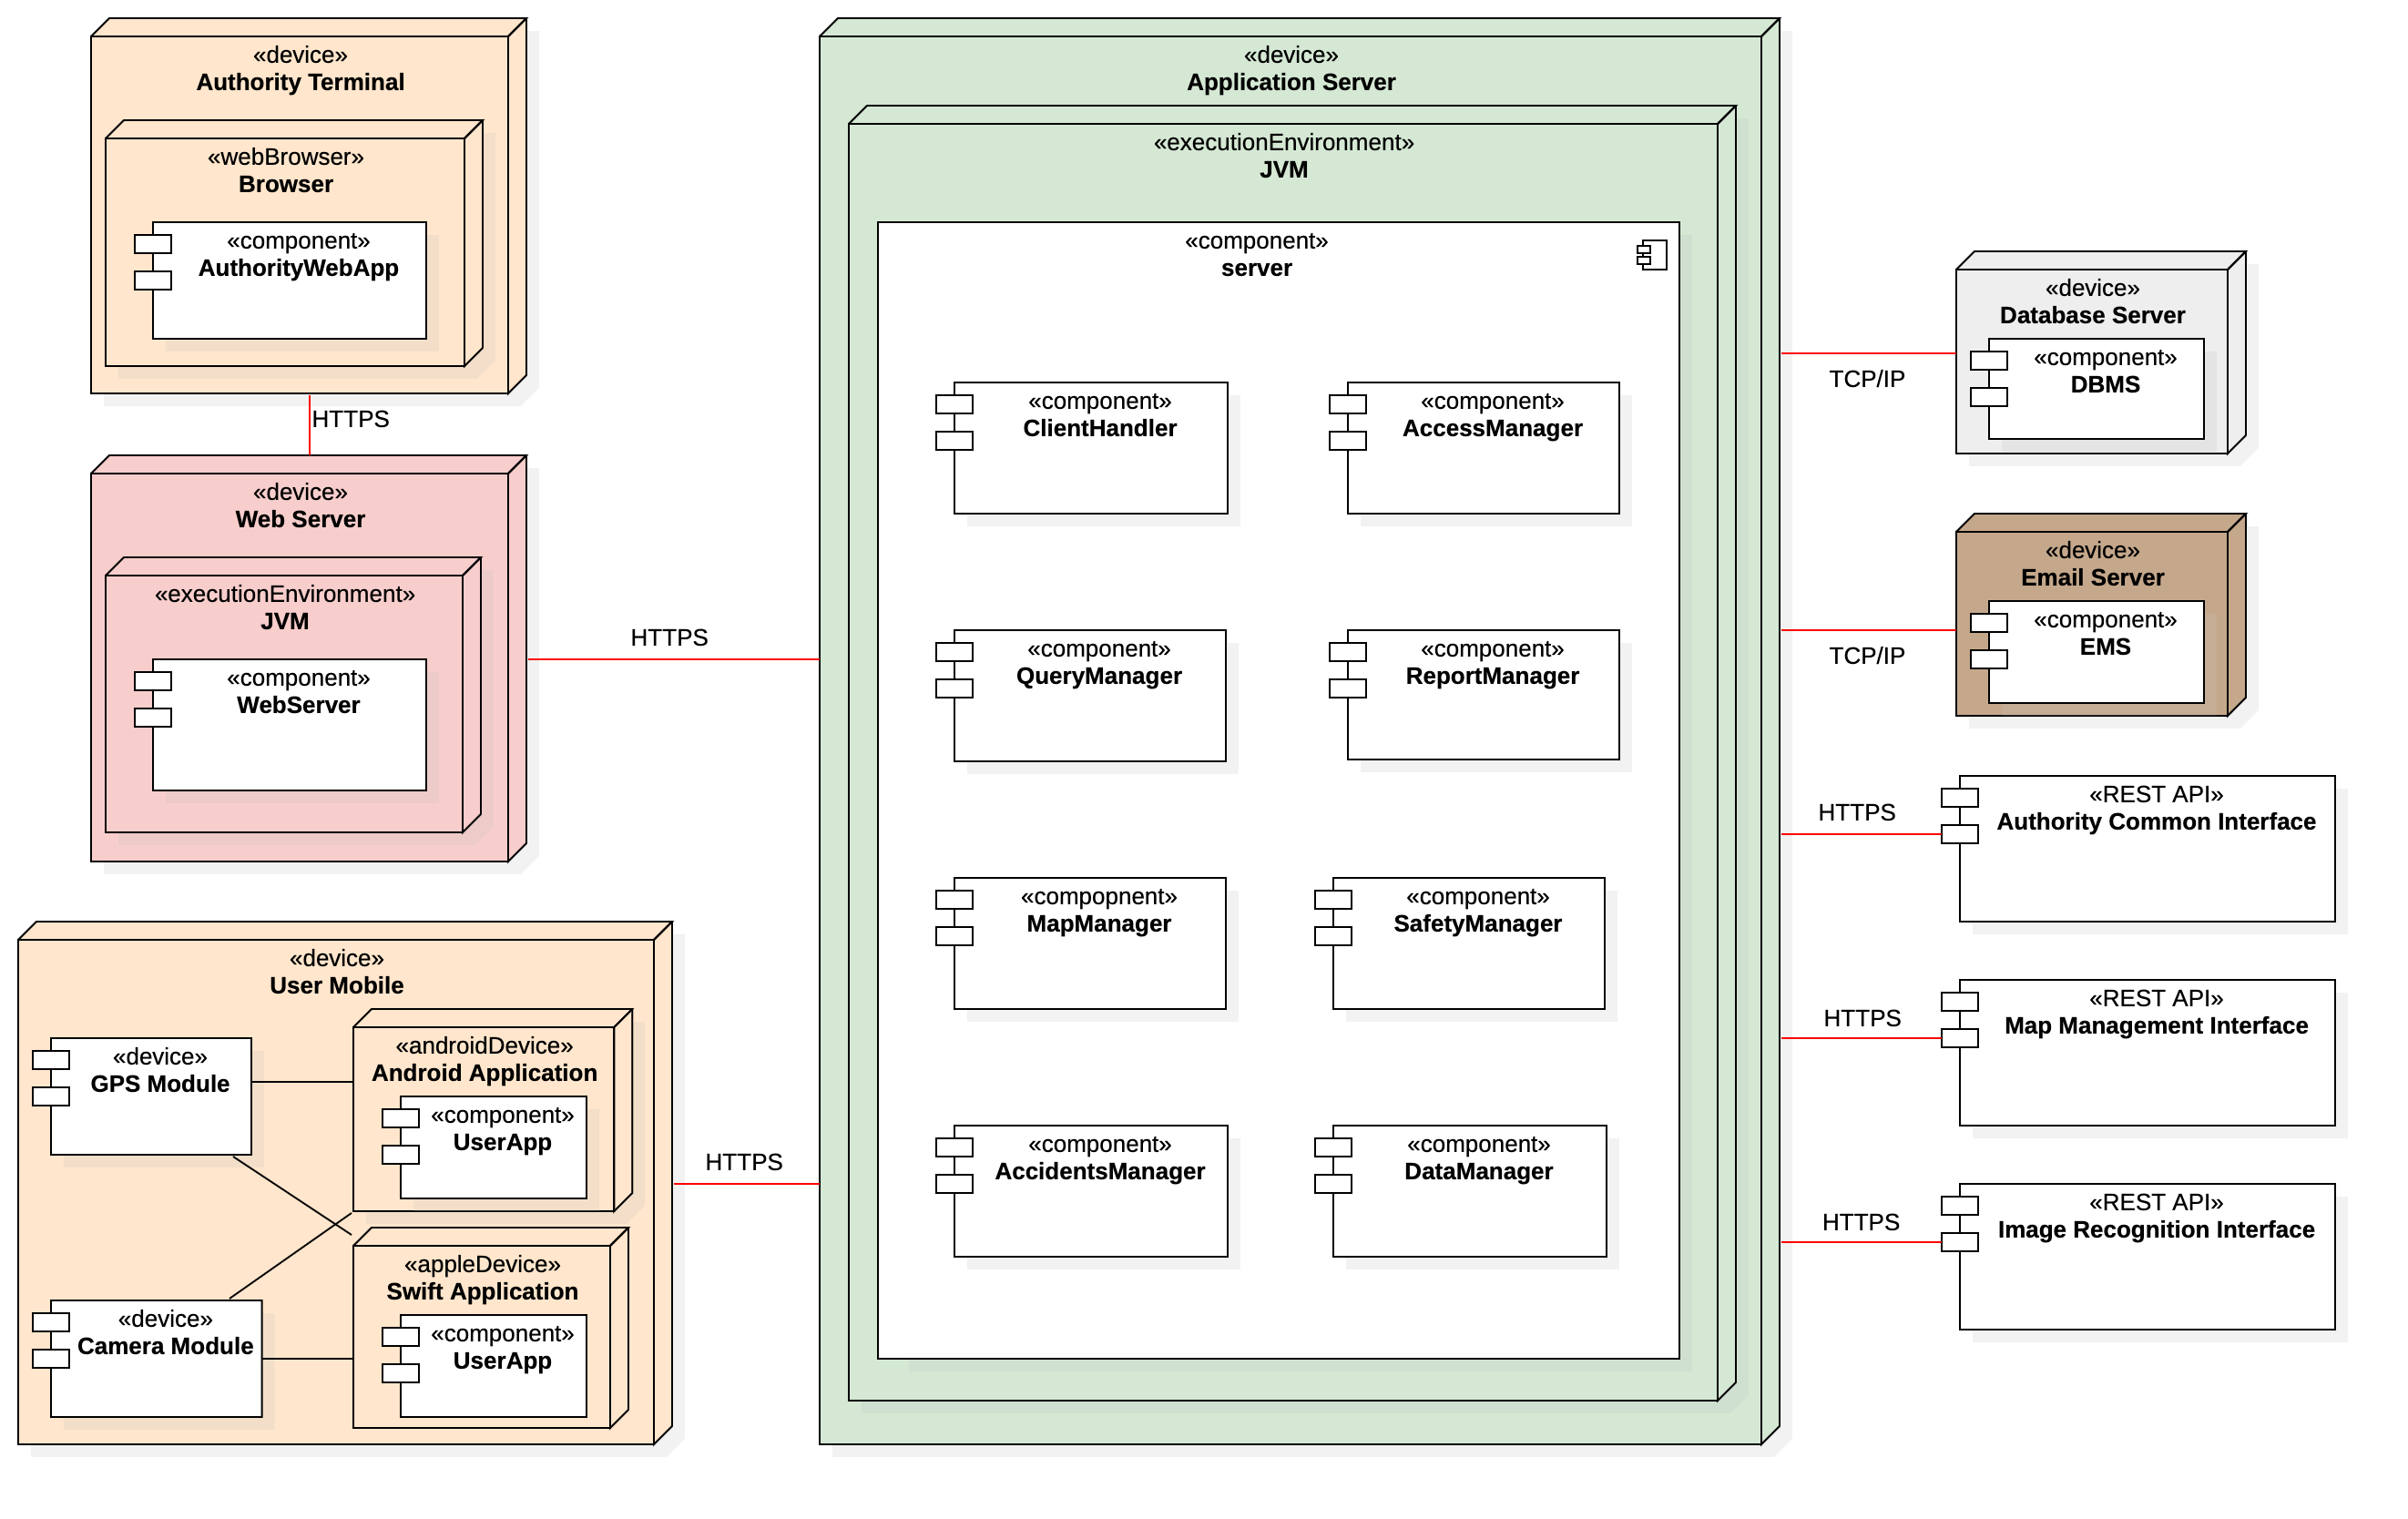
\includegraphics[scale=0.21, angle=90]{/diagrams/deployment/deploymentDiagram.png}
				\caption{\label{fig:deploymentDiagram} Deployment Diagram}
			\end{figure}
		
			\FloatBarrier
			
	\subsection[Runtime View]{\hyperlink{toc}{Runtime View}}
		\label{sec:runtimeView}
		
		In this section we are going to present the most important runtime views of the interactions between customers and SafeStreets. All the methods used in the following diagrams will be precisely described in the next section (\blueRef{sec:componentInterfaces}) where each of them will be mapped to the respective interface that realizes it. For the sake of simplicity we decided to use the first level of components to describe the interactions, in this way we obtained more clear diagrams and their internal correspondence can be easily found with the satisfactory description of every sub-component that we identified in the component view section (\blueRef{sec:componentView}). \\
		
		The \emph{Runtime View Diagrams} of this section are presented first for the \textbf{users} and \textbf{authorities}. Then, for the common functionalities, we decided to show only the interaction between the UserApp and the system to keep the diagrams clear (the ones for the authorities would need an additional interaction with the WebServer before interfacing with the system) and lastly two critical managers are shown in order to present how the components related to the safety and the map issues work.
		
		\subsubsection[User]{\hyperlink{toc}{User}}
			\label{sec:userRuntimeView}
			
			\begin{itemize}
				\item \textbf{Login:} In this sequence diagram (\blueAutoref{fig:loginRuntime}), the process of user login is shown. The authority login is not shown in the runtime view section, since it is basically the same. In fact, both users and authorities log in with a username and a password. This process is actually quite simple: the UserApp asks the server to log in by passing username and password. ClientHandler receives the request and forwards it to the AccessManager component, that will ask DataManager for a simple query in the database. If no user with that username is found, an error message is given to the client, otherwise the check of the password will be performed. If the password inserted and sent by the user is the same as the one retrieved from the database, the login will be considered as logged in and then informed.
				The difference for the authorities is that their login requests will come from  the AuthorityWebApp, instead of using the UserApp, thus the WebServer will be involved too, between the AuthorityWebApp and the ClientHandler.
	
				\item \textbf{Registration:} This sequence diagram (\blueAutoref{fig:userRegistrationRuntime}) pictures the interaction through which a user registers to SafeStreets. After UserApp has asked him all the registration data (username, password, and other information), it will hand them to the server, hidden into a User object. ClientHandler will forward the request to AccessManager, that is the same component that manages the login interactions. AccessManager will first check if there is an already existing user who registered with that same username and in case will send back an error. If not, it will ask DataManager to store the user information into the database of the system.
				
				\newpage
				
				\begin{figure}[h!]
					\centering
					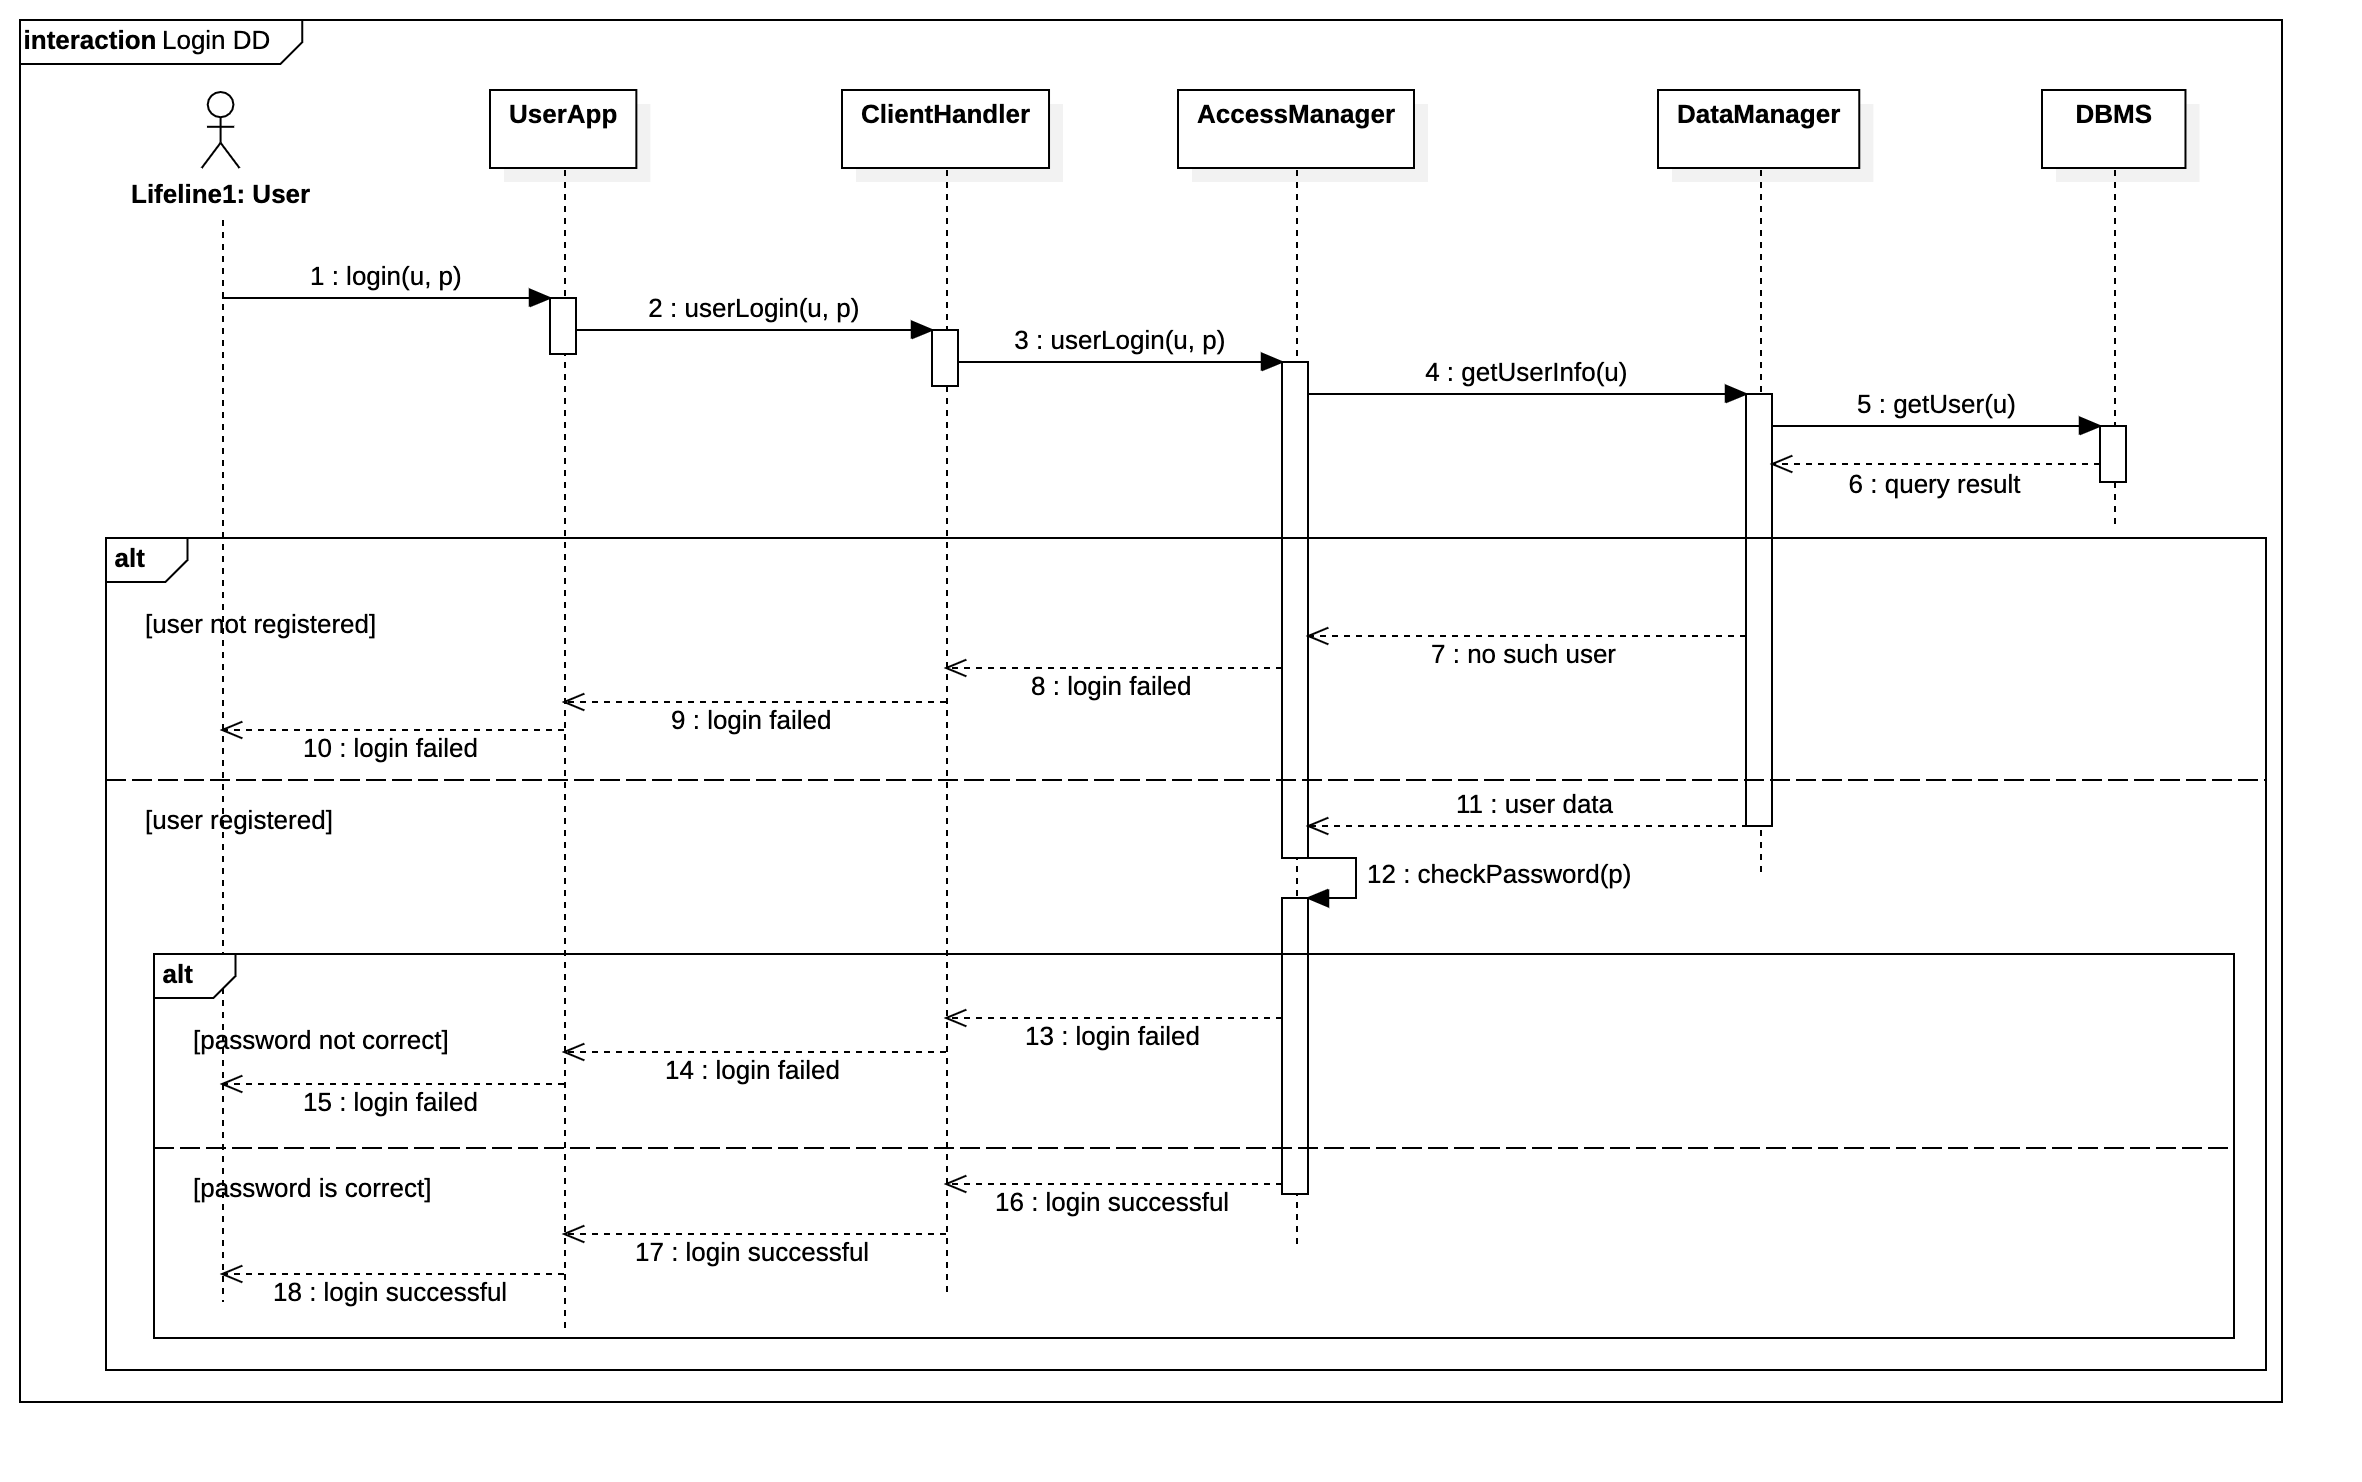
\includegraphics[scale=0.15]{/diagrams/sequence/login.png}
					\caption{\label{fig:loginRuntime} Login Runtime View}
				\end{figure}
			
				\vspace{2cm}
				
				\begin{figure}[h!]
					\centering
					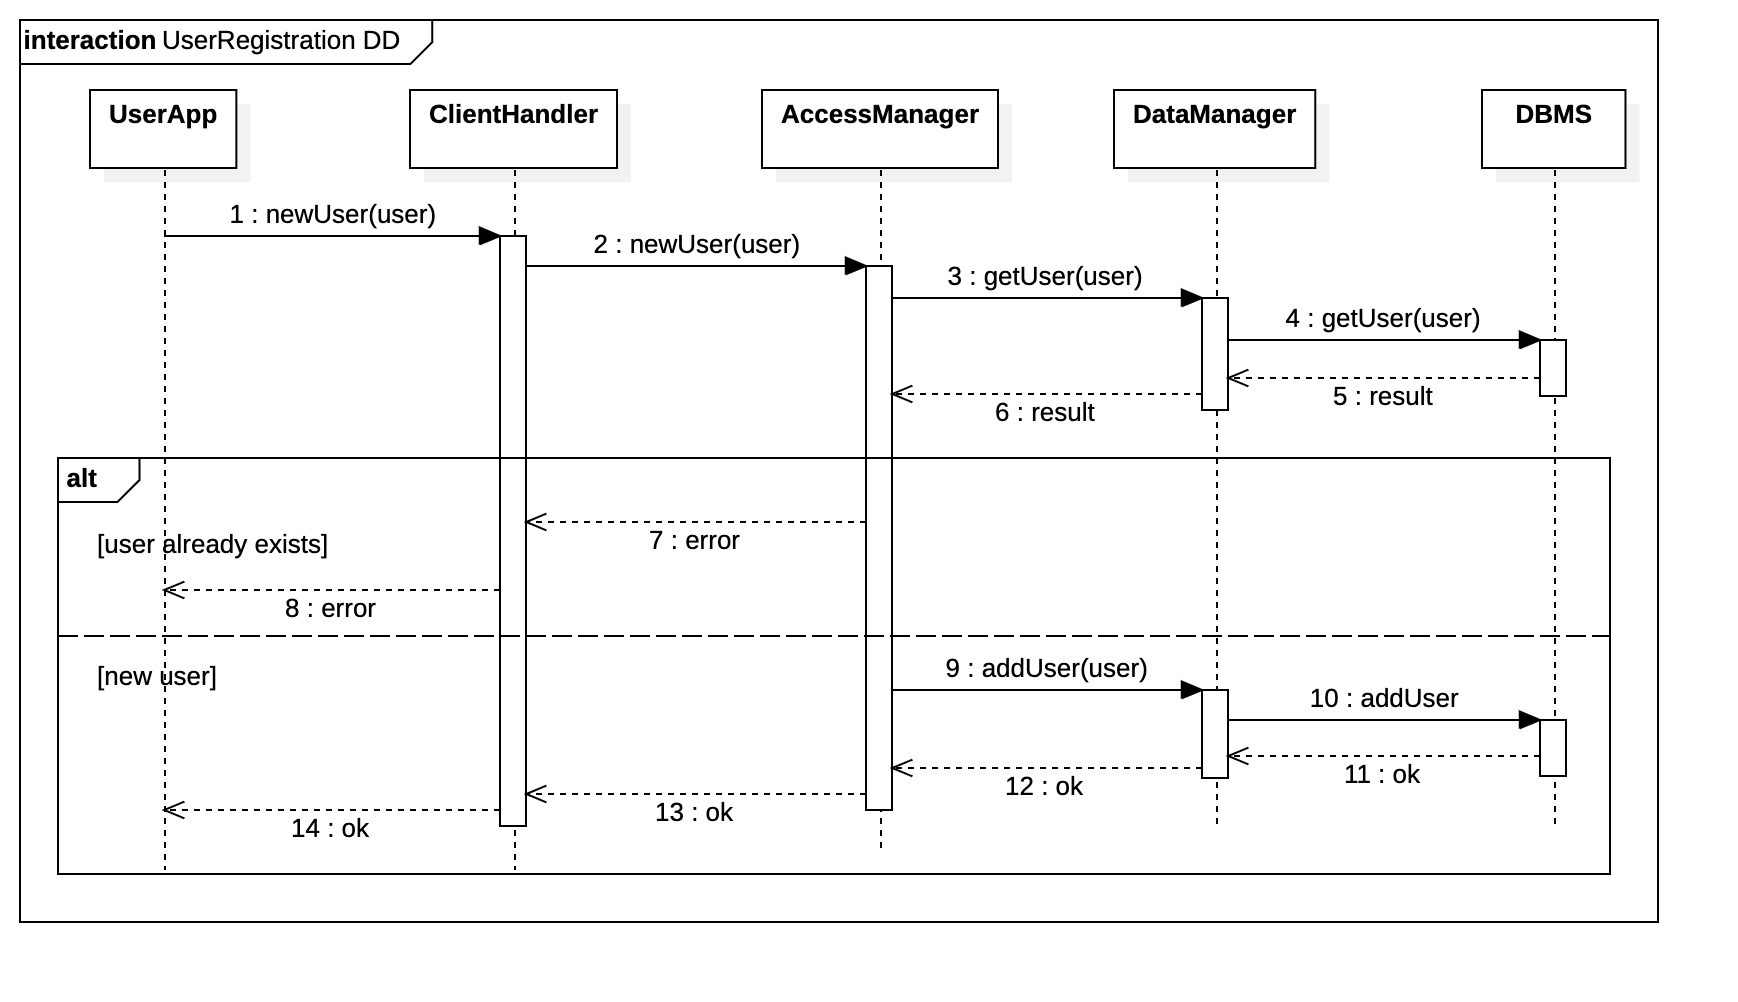
\includegraphics[scale=0.21]{/diagrams/sequence/userRegistration.png}
					\caption{\label{fig:userRegistrationRuntime} User Registration Runtime View}
				\end{figure}
			
				\FloatBarrier
				\newpage
			
				\item \textbf{Report Violation:} Here (\blueAutoref{fig:reportViolationRuntime}), it is shown how a violation is reported by users to the system. UserApp sends all the information contained in a Violation object (pictures, location, ...). ClientHandler forwards the call to ReportManager, the component designed to handle the reports. It will indeed ask IRI for the plate number, providing it with the pictures sent by the user. Then, it will ask MapManager for the name of the street of the violation. MapManager of course needs to ask the external MI to accomplish this, and it only needs the provided location. When all the information is gathered, the report is ready to be stored into the database. To do so, ReportManager will ask DataManager to interact with the DBMS and update the related table(s).
				
				\begin{figure}[h!]
					\centering
					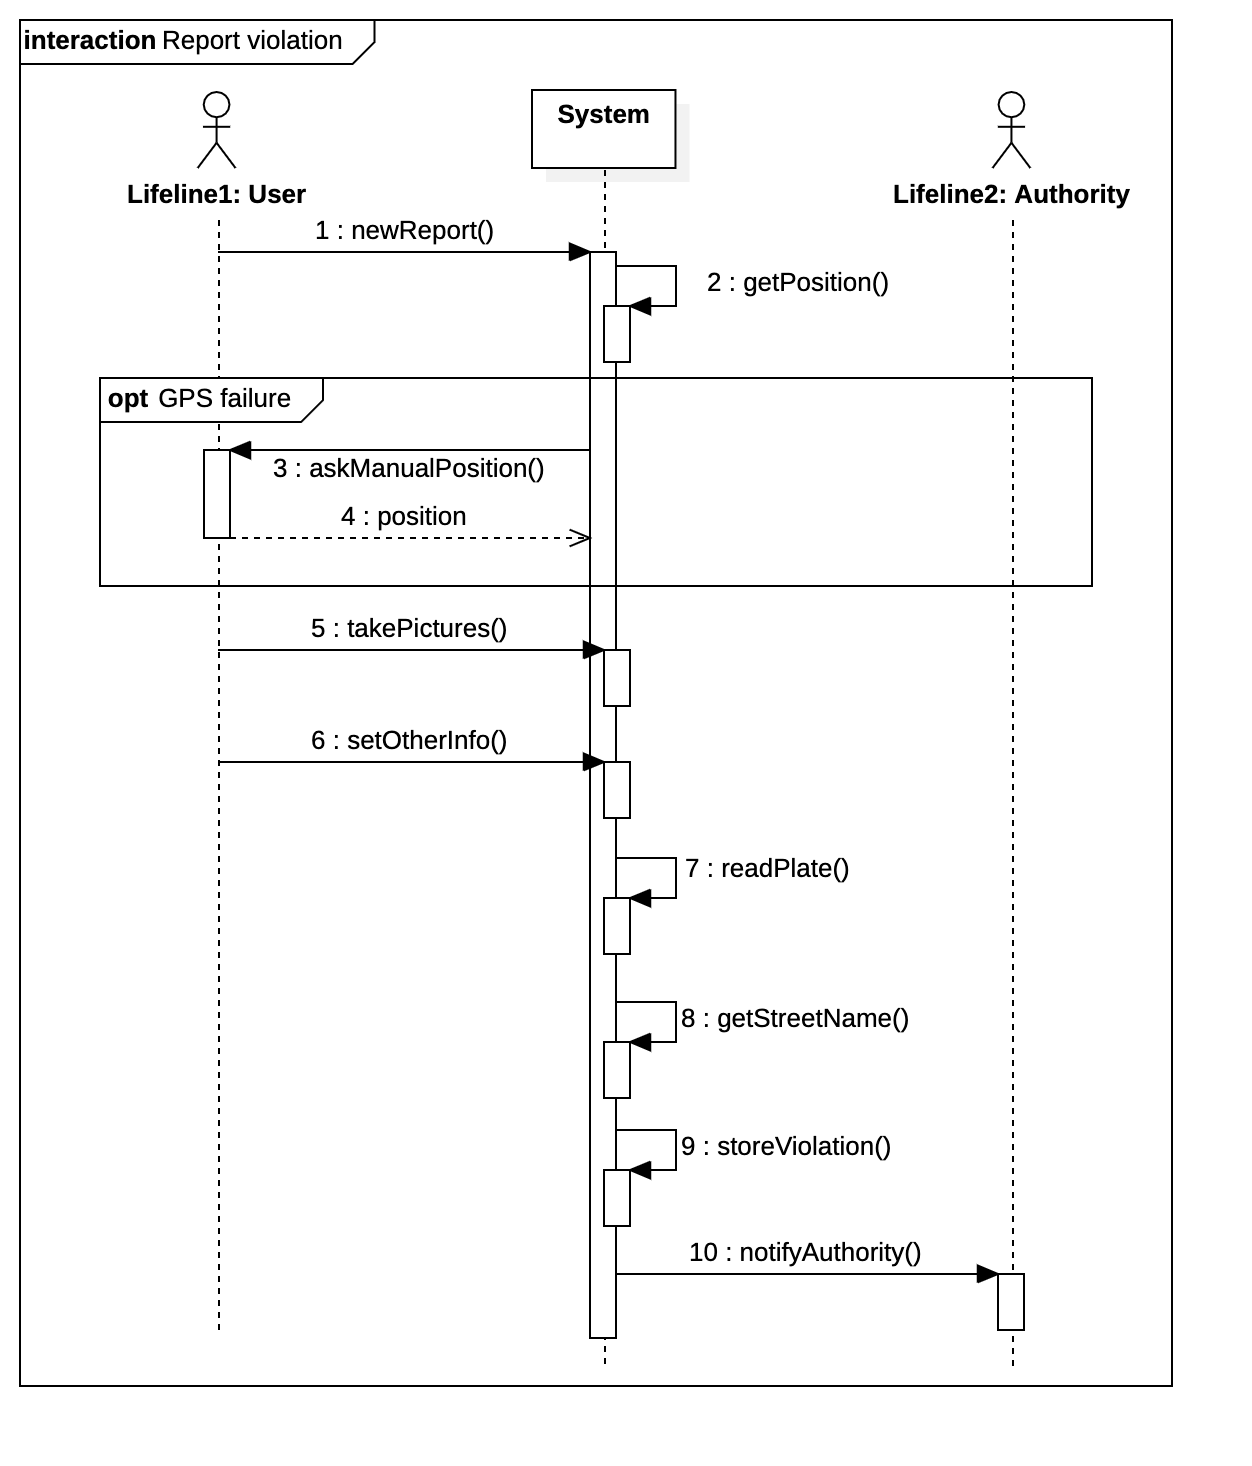
\includegraphics[scale=0.15]{/diagrams/sequence/reportViolation.png}
					\caption{\label{fig:reportViolationRuntime} Report Violation Runtime View}
				\end{figure}
			\end{itemize}
		
		\subsubsection[Authority]{\hyperlink{toc}{Authority}}
			\label{sec:authorityRuntimeView}
			
			The following are the interactions that involve authorities. In the sequence diagrams, all of these interactions start with a call from the WebServer but of course, the component that really starts them is the AuthorityWebApp, that asks web pages to the WebServer. The interaction between the AuthorityWebApp and the WebServer is not shown here for the sake of simplicity.
			
			\begin{itemize}
				\item \textbf{Registration:} It is now described (\blueAutoref{fig:authorityRegistrationRuntime}) the process through which an authority registers to SafeStreets. This is a little bit more complicated process with respect to the user one, because the system requires the authority to be real and recognized. The assumption here is that there's a completely secure PEC address assigning mechanism. The ClientHandler forwards the WebServer request to AccessManager. The request contains of course all the necessary information for the registration. AccessManager will then check whether there is already an authority registered for the city contained in the registration request. If a authority already exists, the request is rejected and an error message is sent back to the client, otherwise AccessManager will check whether the specified PEC address actually corresponds to the authority of the city contained in the request. This is to avoid that an authority registers for a different city. To do that, it needs to ask the Authority Common Interface that is external with respect to SafeStreets. If the addresses do not match, an error message is sent to the client and the procedure is aborted. If the specified address is correct for that city, SafeStreets needs now to verify that the actual person that is making the request through the AuthorityWebApp is able to access the PEC address and actually read the received emails. In order to do that, AccessManager generates a code that will be sent by PEC through EmailAPI. AccessManager now waits for the authority to insert, through the AuthorityWebApp, the received code. Then, it will check that the generated code and the inserted one coincide. If they do not coincide, an error is sent to the AuthorityWebApp and the registration is aborted. If the inserted code is correct, AccessManager will ask DataManager to store the information into the database.
				
				\begin{figure}[h!]
					\centering
					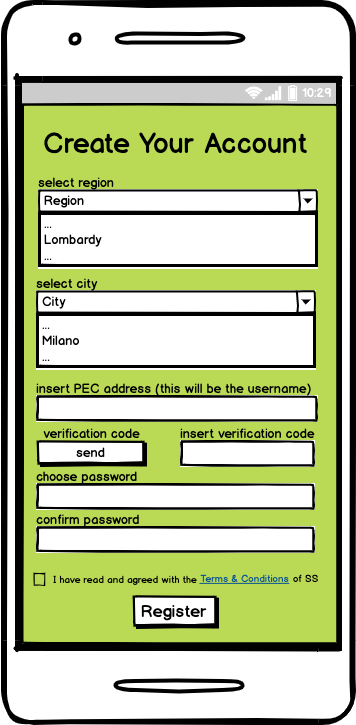
\includegraphics[scale=0.14]{/diagrams/sequence/authorityRegistration.png}
					\caption{\label{fig:authorityRegistrationRuntime} Authority Registration Runtime View}
				\end{figure}
			
				\item \textbf{Check Unread Reports:} In this sequence diagram (\blueAutoref{fig:unreadReportsRuntime}), it is shown how an authority is able to retrieve all the unread reports sent by users to SafeStreets. The WebServer will ask ClientHandler to forward the request to the right component, that in this case is again QueryManager. In fact, its job is to call the right method of DataManager to obtain only the reports that have the "read" flag set to false. DataManager will as usual execute the actual query into the DBMS. Finally, QueryManager will send the result back to the WebServer, that will forward it to the AuthorityWebApp.
				
				\begin{figure}[h!]
					\centering
					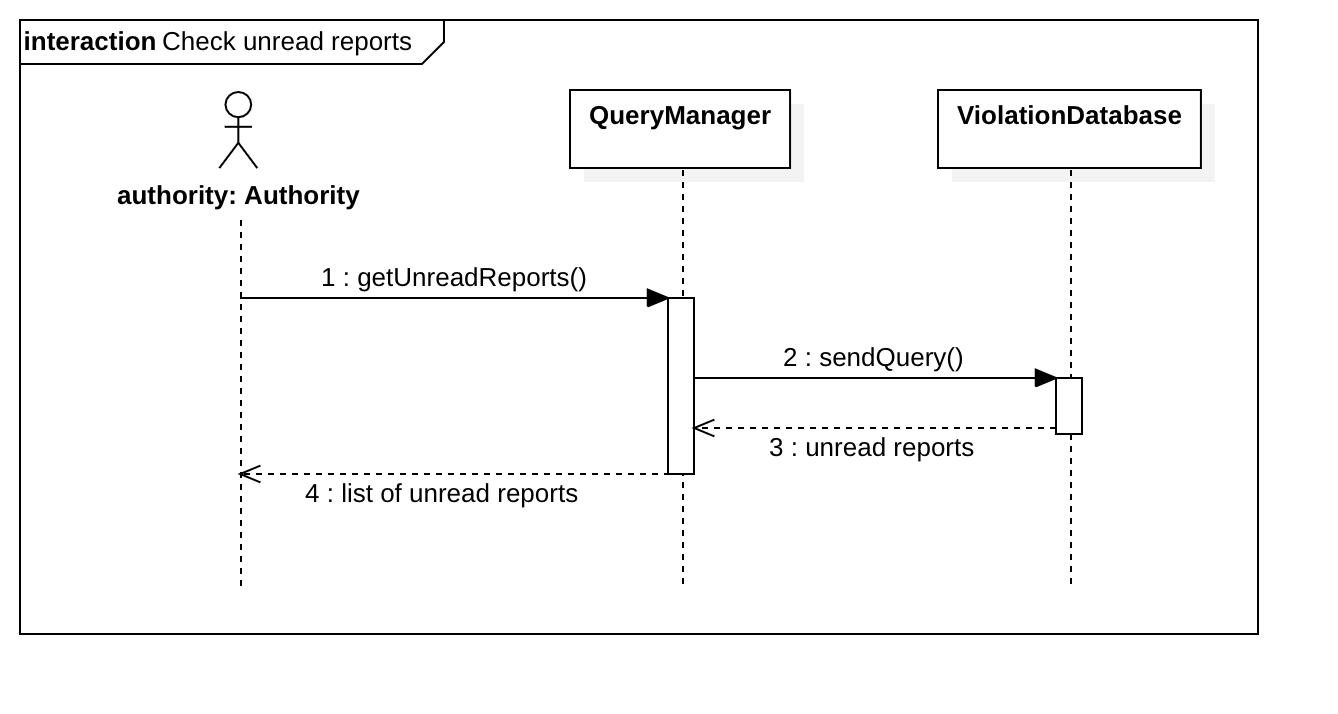
\includegraphics[scale=0.17]{/diagrams/sequence/unreadReports.png}
					\caption{\label{fig:unreadReportsRuntime} Check Unread Reports Runtime View}
				\end{figure}
			
				\item \textbf{Find Reports:} Here (\blueAutoref{fig:findReportsRuntime}) we describe the interactions between the components when the authority asks for some past reports applying some filters. The request is made by the WebServer and is forwarded to QueryManager by ClientHandler. After having checked if the specified filters are correct and eventually returning an error to the AuthorityWebApp, QueryManager will ask DataManager to interact with the DBMS and execute the query that will return all the reports located in the authority’s city that match the specified filters.
				
				\begin{figure}[h!]
					\centering
					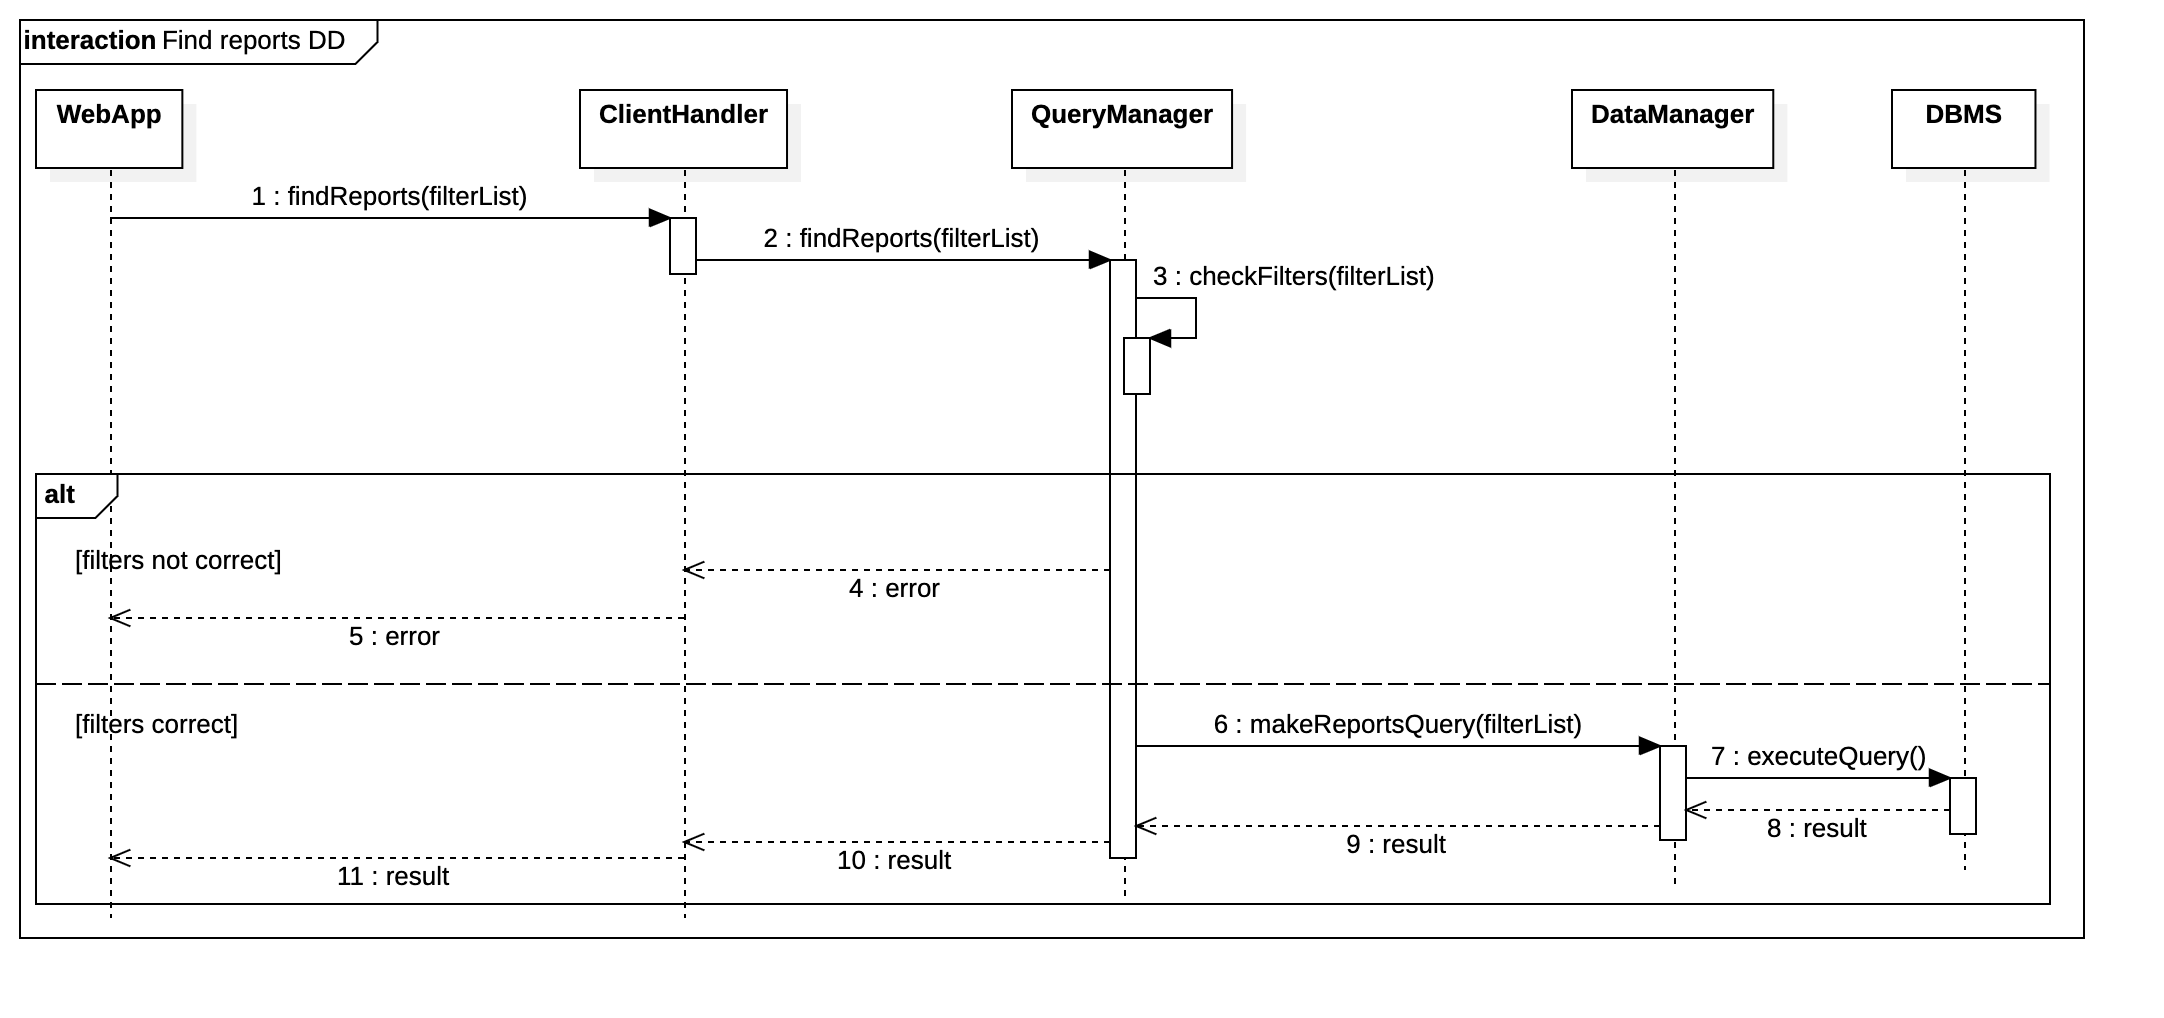
\includegraphics[scale=0.17]{/diagrams/sequence/findReports.png}
					\caption{\label{fig:findReportsRuntime} Find Reports Runtime View}
				\end{figure}
			\end{itemize}
		
		\subsubsection[Common Functionalities]{\hyperlink{toc}{Common Functionalities}}
			\label{sec:commonFunctionalitiesRuntime}
			
			These functionalities are available to both users and authorities. Therefore, they're reported here.
			
			\begin{itemize}
				\item \textbf{Find Streets With Highest Number of Violations:} It is now shown (\blueAutoref{fig:violationsFrequencyRuntime}) how a possible query for the streets with the highest number of violations is made. The filterList object represents all the filters that are selected by the user, like time slots and types of violation. These filters are widely described in the RASD. The component designed to handle these queries is of course QueryManager. It will check the correctness of all the used filters (e.g. at least a type of violation must be included). If some constraint is not fulfilled, an error is sent to the user, otherwise QueryManager will prepare the query and forward it to DataManager, that will actually execute it on the DBMS. The result is then back propagated through the involved components and to the UserApp.
				
				\begin{figure}[h!]
					\centering
					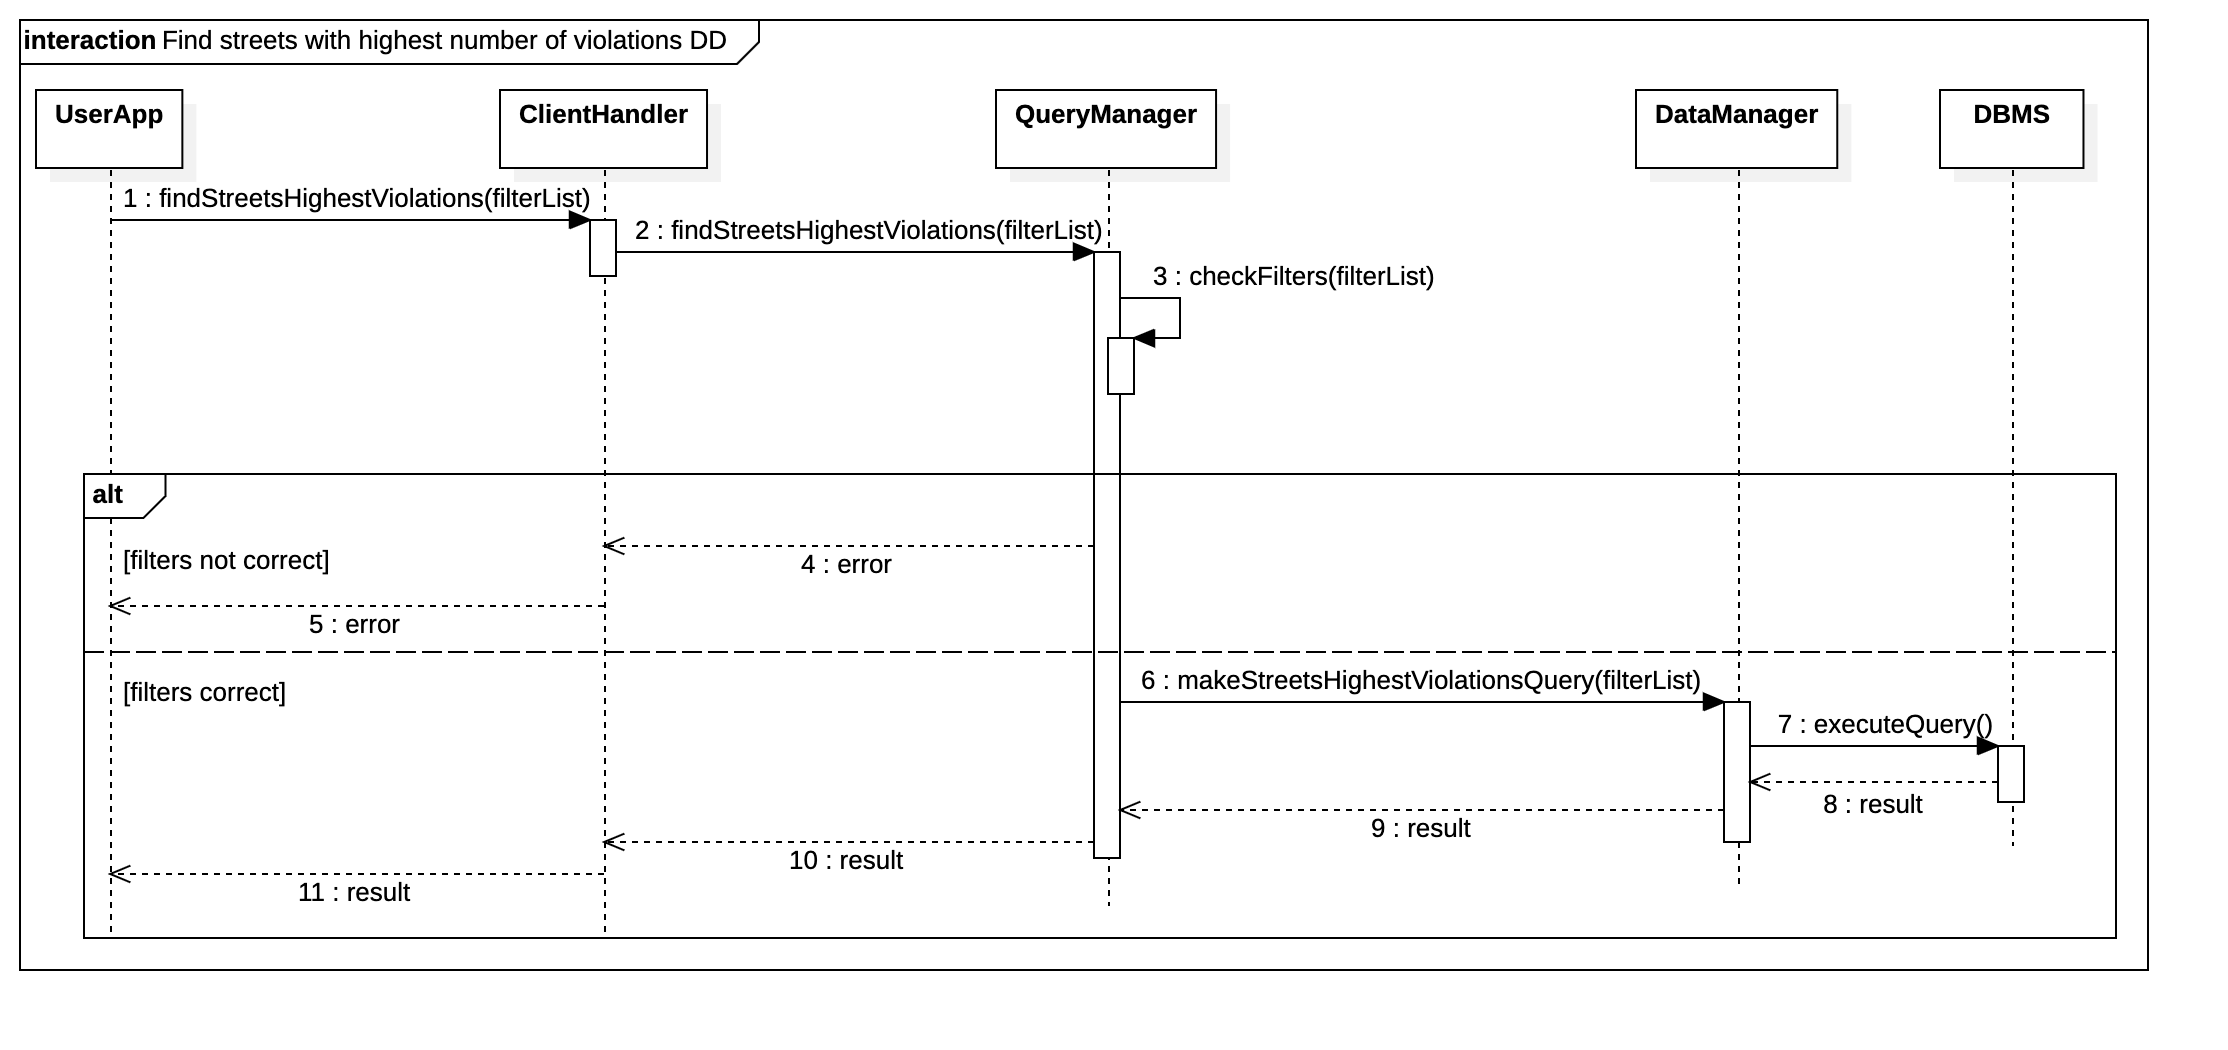
\includegraphics[scale=0.16]{/diagrams/sequence/violationsFrequency.png}
					\caption{\label{fig:violationsFrequencyRuntime} Violations Frequency Runtime View}
				\end{figure}
			
				\item \textbf{Find Dangerous Vehicles:} This interaction (\blueAutoref{fig:dangerousVehiclesRuntime}) is basically the same as the previous one, thus it won't be explained again here. The only difference is that the query designed by QueryManager will be specific for finding the types of vehicle that made the most violations.
				
				\begin{figure}[h!]
					\centering
					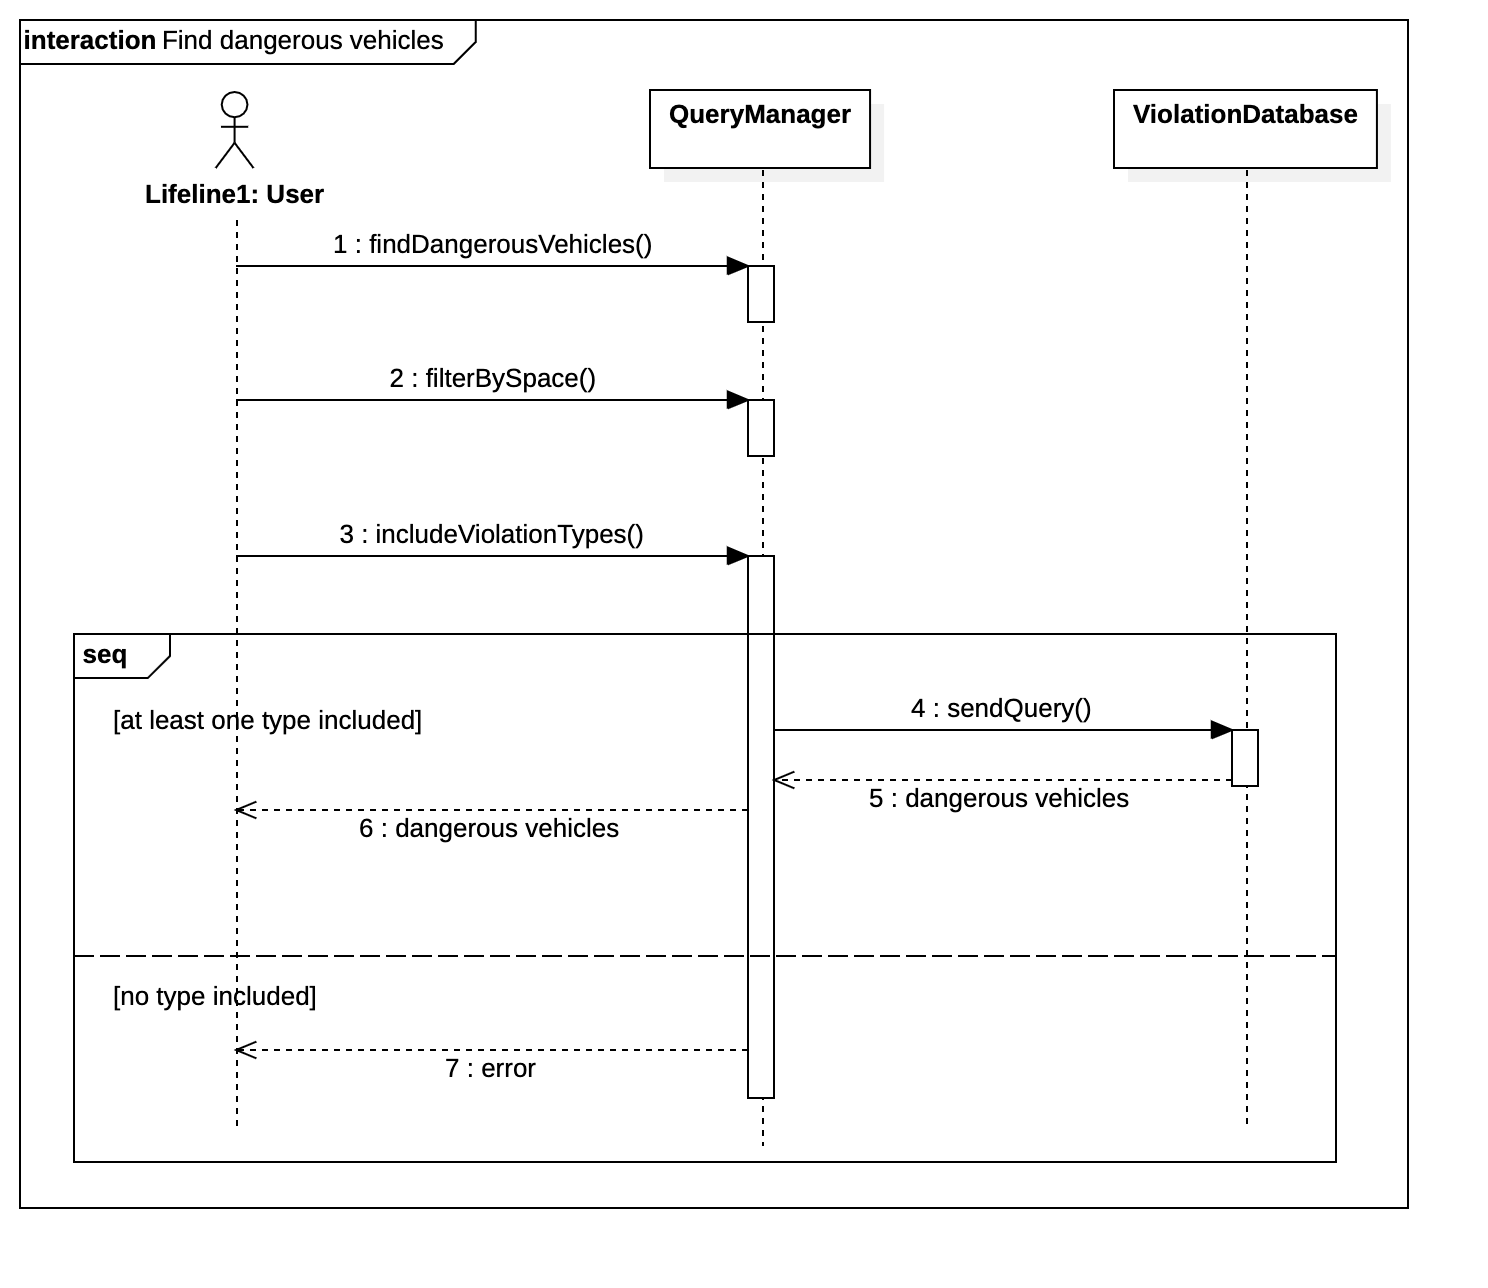
\includegraphics[scale=0.17]{/diagrams/sequence/dangerousVehicles.png}
					\caption{\label{fig:dangerousVehiclesRuntime} Dangerous Vehicles Runtime View}
				\end{figure}
			
				\item \textbf{Find Unsafe Streets:} In this interaction (\blueAutoref{fig:unsafeStreetsRuntime}) it is shown how the UserApp requests maps with coloured streets. The request made by the UserApp is forwarded by ClientHandler to QueryManager. Depending on the option selected by the user, three different methods could be called: the one with a city as input, the one with starting and ending points, or the one with a single street. In the first case, QueryManager will look for all the streets of the selected city in the DBMS, going through DataManager. In the second case, a path needs to be generated, thus QueryManager will ask MI through MapManager for a path, that will include a certain number of streets. In the last case, no action is required. Then, for all the gathered streets, QueryManager will search in the database for their safety, asking DataManager to execute the actual query. Then QueryManager will ask MapManager for the generation of the map that, according to the gathered infomation about the safety of the involved streets, will be coloured as described in RASD. If path option was selected, the path will be passed to MapInterface so that the generated map will show it. This map will be finally sent back to the UserApp and displayed.
				
				\vspace{1cm}		
		
				\begin{figure}[h!]
					\centering
					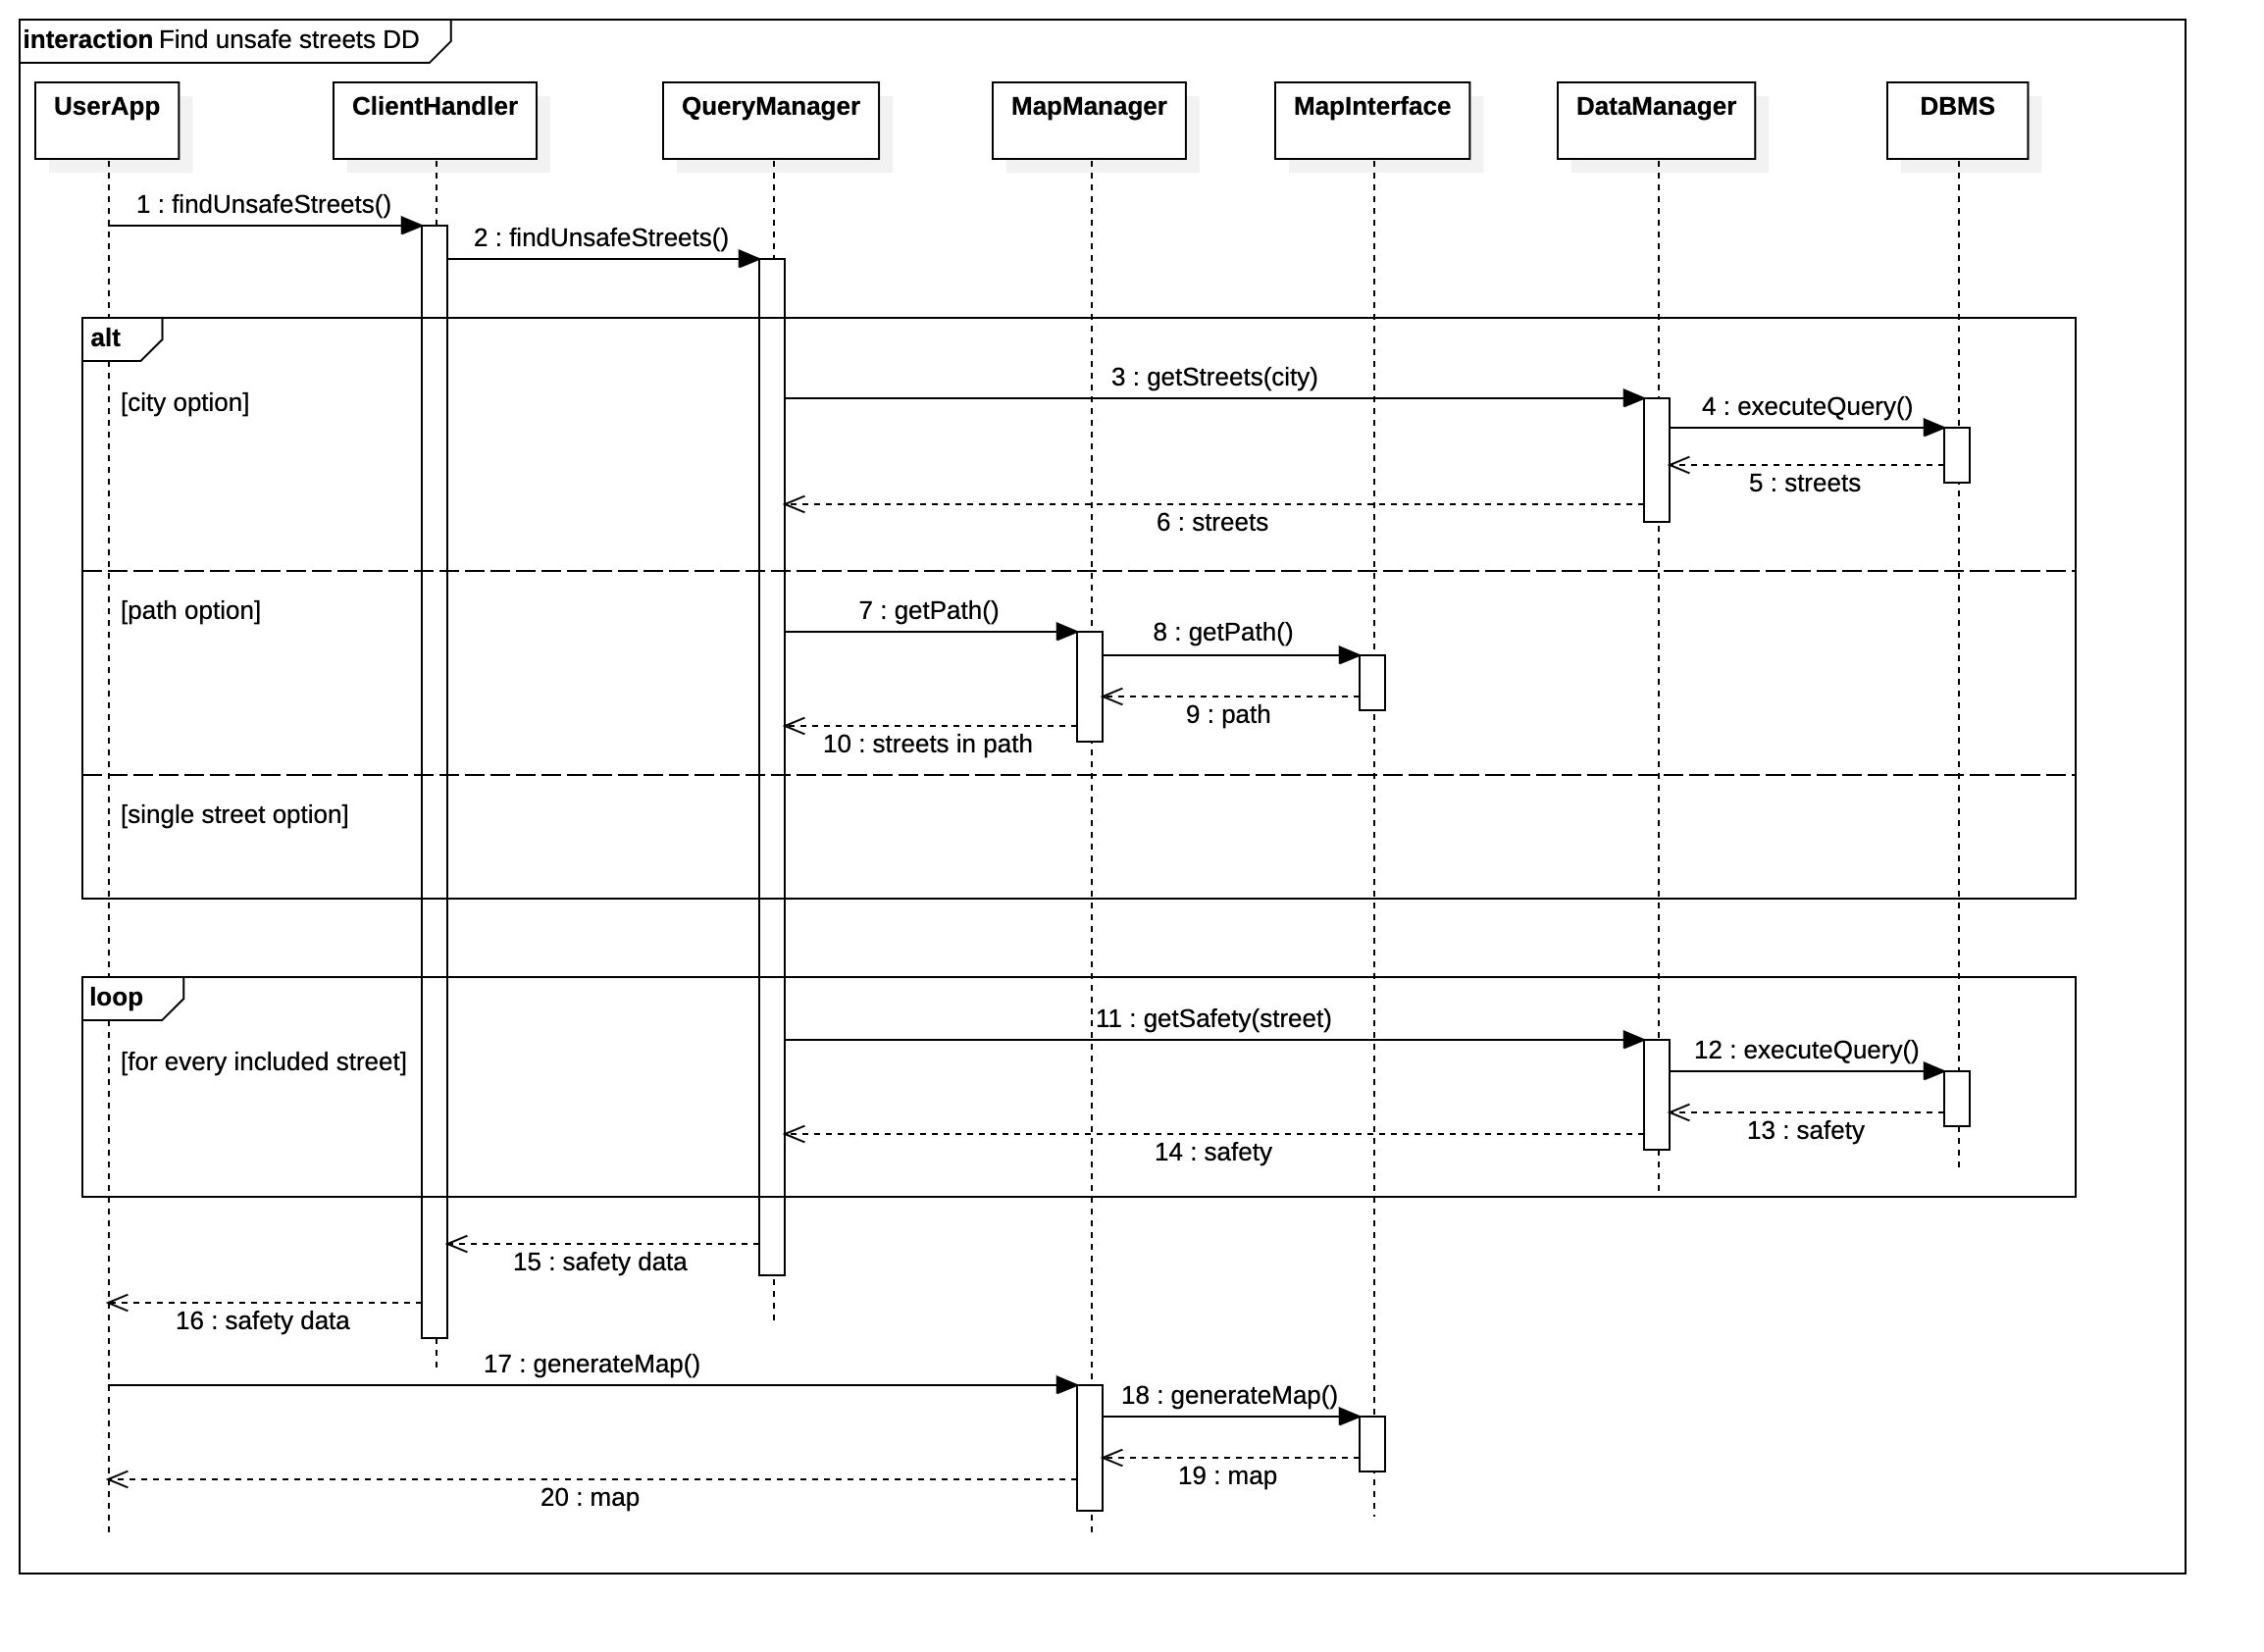
\includegraphics[scale=0.17]{/diagrams/sequence/unsafeStreets.png}
					\caption{\label{fig:unsafeStreetsRuntime} Unsafe Streets Runtime View}
				\end{figure}
			
				\newpage
			
				\item \textbf{Find Urgent Interventions:} This interaction (\blueAutoref{fig:urgentInterventionsRuntime}) is basically the same as "find streets with highest number of violations", thus it won't be explained again here. The only difference is that the query designed by QueryManager will be specific for urgent interventions.
				
				\begin{figure}[h!]
					\centering
					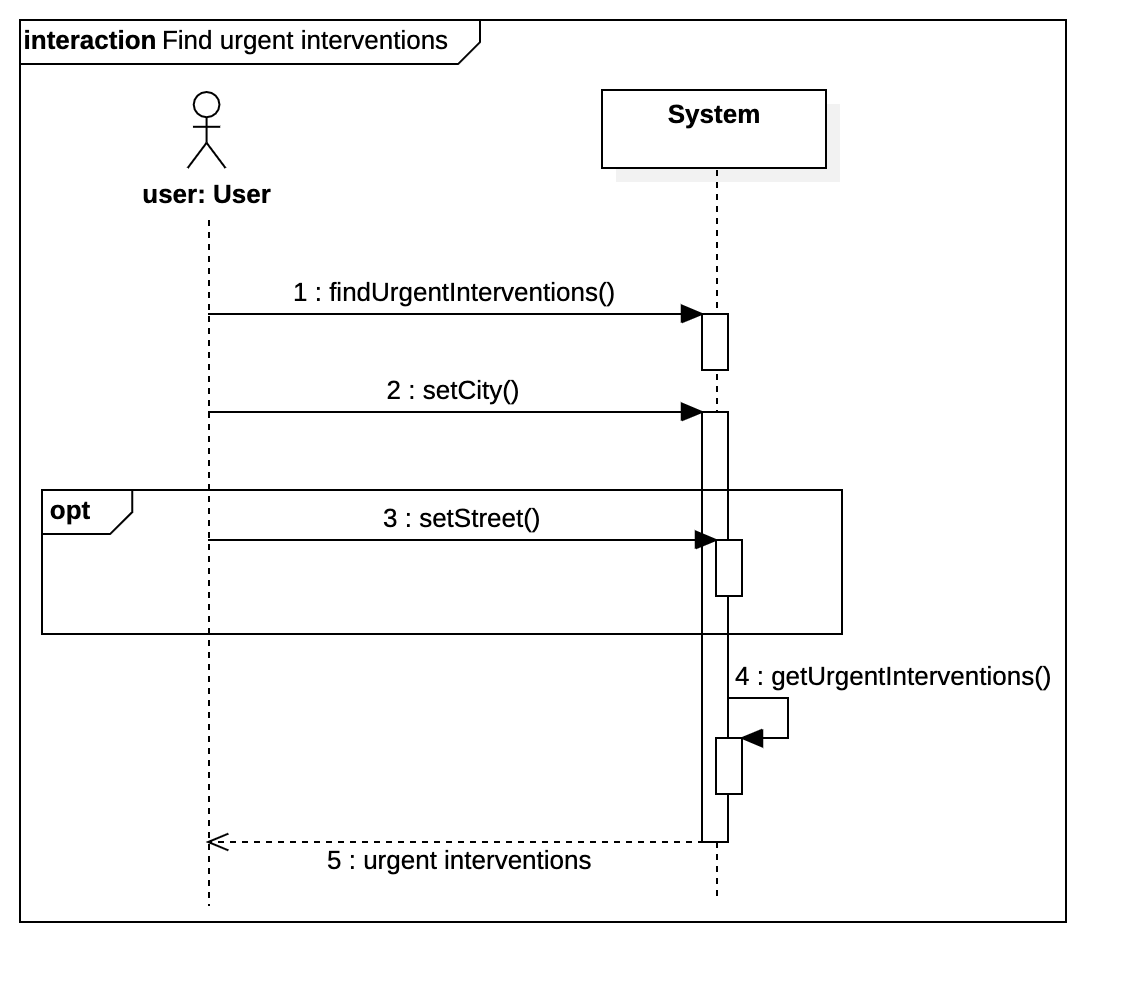
\includegraphics[scale=0.17]{/diagrams/sequence/urgentInterventions.png}
					\caption{\label{fig:urgentInterventionsRuntime} Urgent Interventions Runtime View}
				\end{figure}
			\end{itemize}
		
			\FloatBarrier
		
		\subsubsection[Safety Manager]{\hyperlink{toc}{Safety Manager}}
			\label{sec.safetyManagerRuntime}
			
			\begin{itemize}
				\item \textbf{Update Safety:} This  (\blueAutoref{fig:safetyUpdateRuntime}) is the description of the process of updating the safety estimation of every registered street, along with the suggested possible interventions. The component designed to do this operation is SafetyManager. It asks DataManager to get all the violations and accidents information from the DBMS. Then it will calculate the safety estimation and all the possible interventions for that street as described in RASD. Finally, it will store safety estimation and all those possible interventions in the database, so that it will be possible to always retrieve the most updated information without actually calculating it for every request that is made.
				
				\begin{figure}[h!]
					\centering
					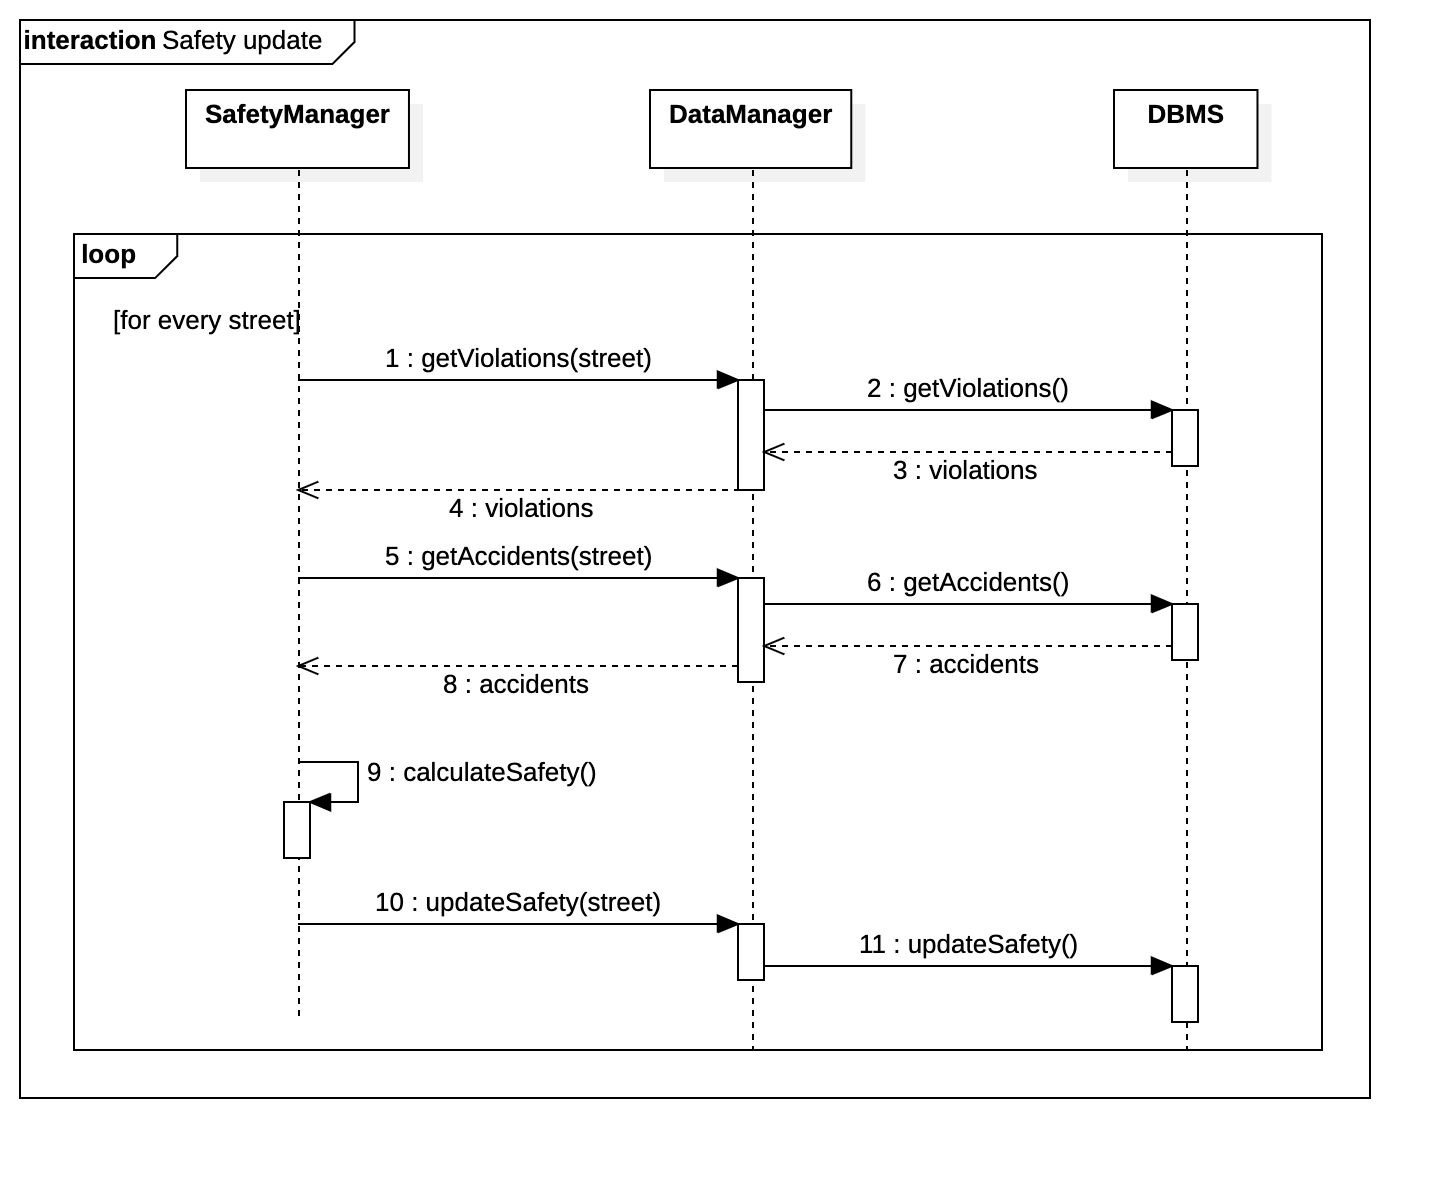
\includegraphics[scale=0.21]{/diagrams/sequence/safetyUpdate.png}
					\caption{\label{fig:safetyUpdateRuntime} Update Safety Runtime View}
				\end{figure}
			
				\item \textbf{Update Accidents:} Here (\blueAutoref{fig:accidentsUpdateRuntime}) it is described how SafeStreets uses the Authority Common Interface to retrieve data about accidents. For every city with a registered authority, AccidentsManager will ask ACI for these data and then will ask DataManager to store them into the database.
				
				\begin{figure}[h!]
					\centering
					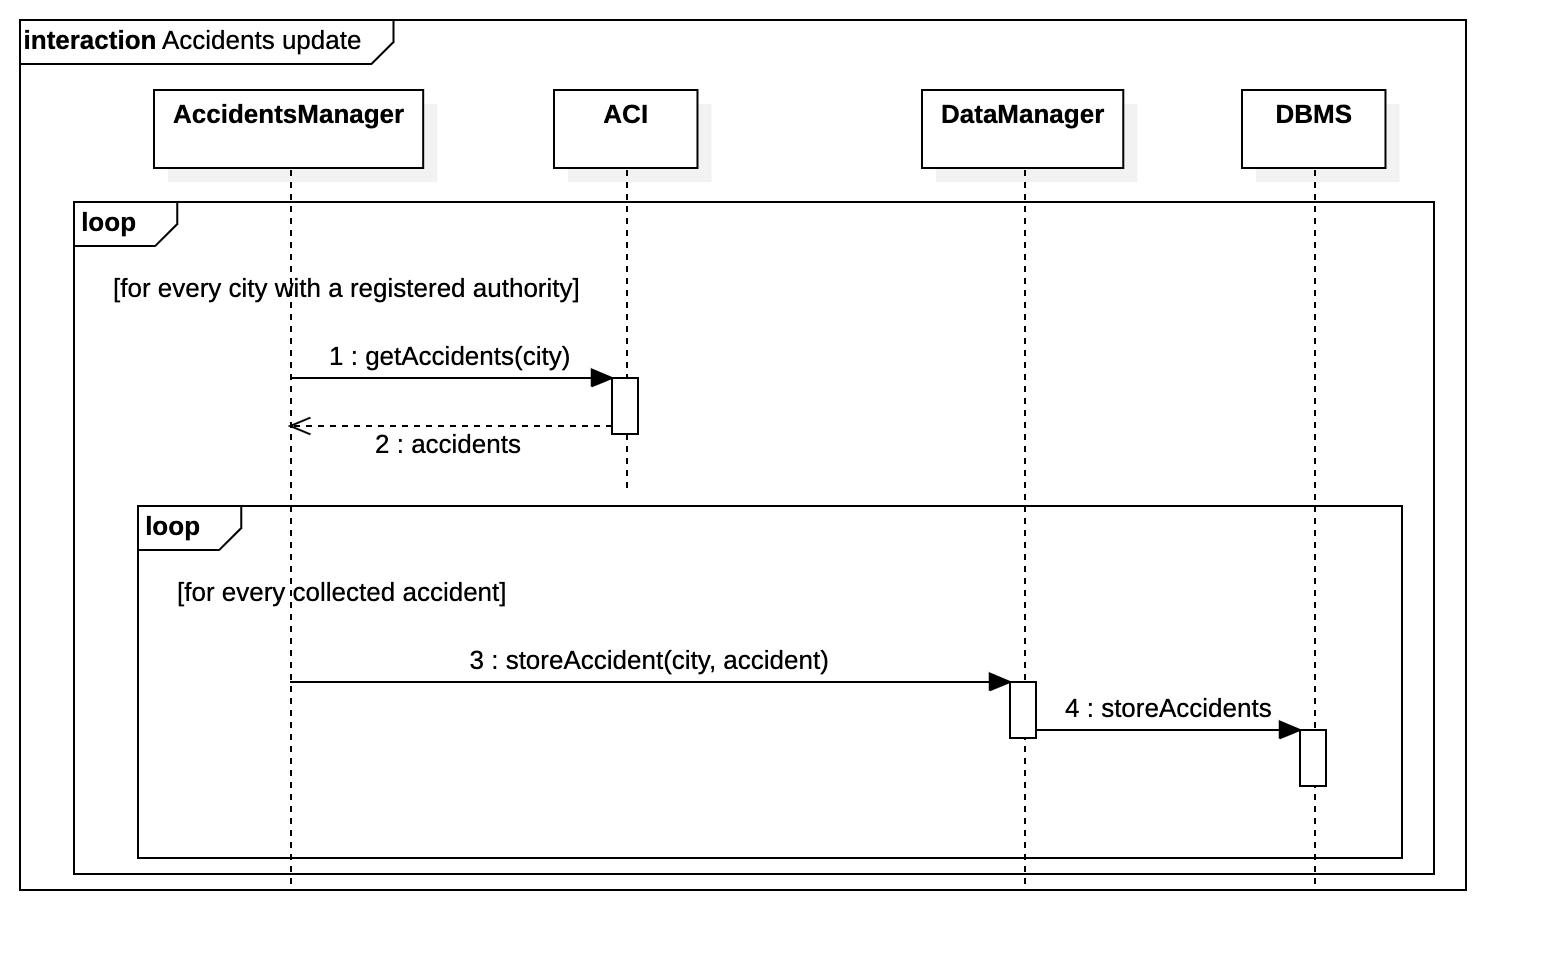
\includegraphics[scale=0.21]{/diagrams/sequence/accidentsUpdate.png}
					\caption{\label{fig:accidentsUpdateRuntime} Update Accidents Runtime View}
				\end{figure}
			\end{itemize}
		
			\FloatBarrier
		
		\subsubsection[Map Manager]{\hyperlink{toc}{Map Manager}}
		\label{sec:mapManagerRuntime}
		
		The map manager has to deal with a particular component that deals with the updating of the information related to the maps it has stored in the databases. This is the diagram (\blueAutoref{fig:mapUpdateRuntime}) describes the updating process of the map thanks to the component designed for this operation: the \emph{MapManager}. It asks the external MapInterface for an updated map of the whole territory considered by SafeStreets and then stores it in the database. What is stored is actually a simpler version of the map: all the system needs is in fact the collection of cities and streets and the relationships among them.
		
		\begin{figure}[h!]
			\centering
			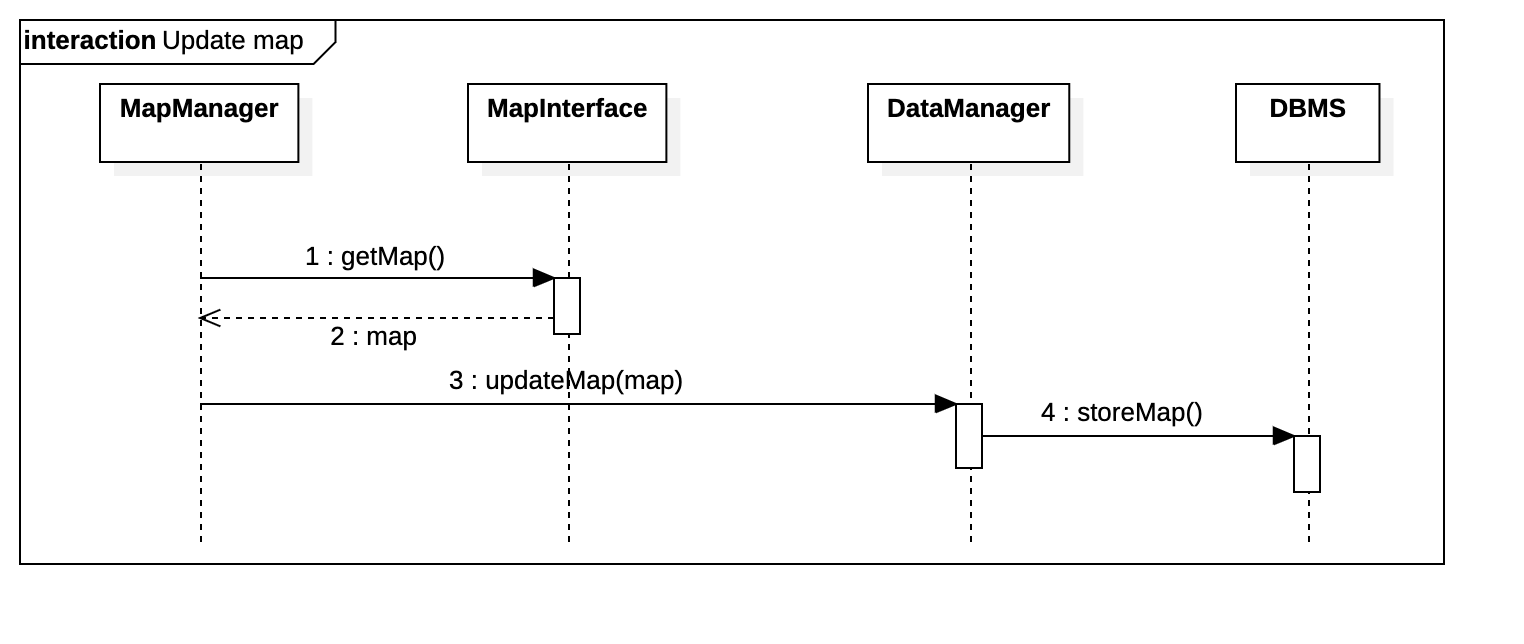
\includegraphics[scale=0.24]{/diagrams/sequence/mapUpdate.png}
			\caption{\label{fig:mapUpdateRuntime} Update Map Runtime View}
		\end{figure}		
	
	\subsection[Component Interfaces]{\hyperlink{toc}{Component Interfaces}}
		\label{sec:componentInterfaces}
		
		\begin{figure}[hbtp]
			\centering
			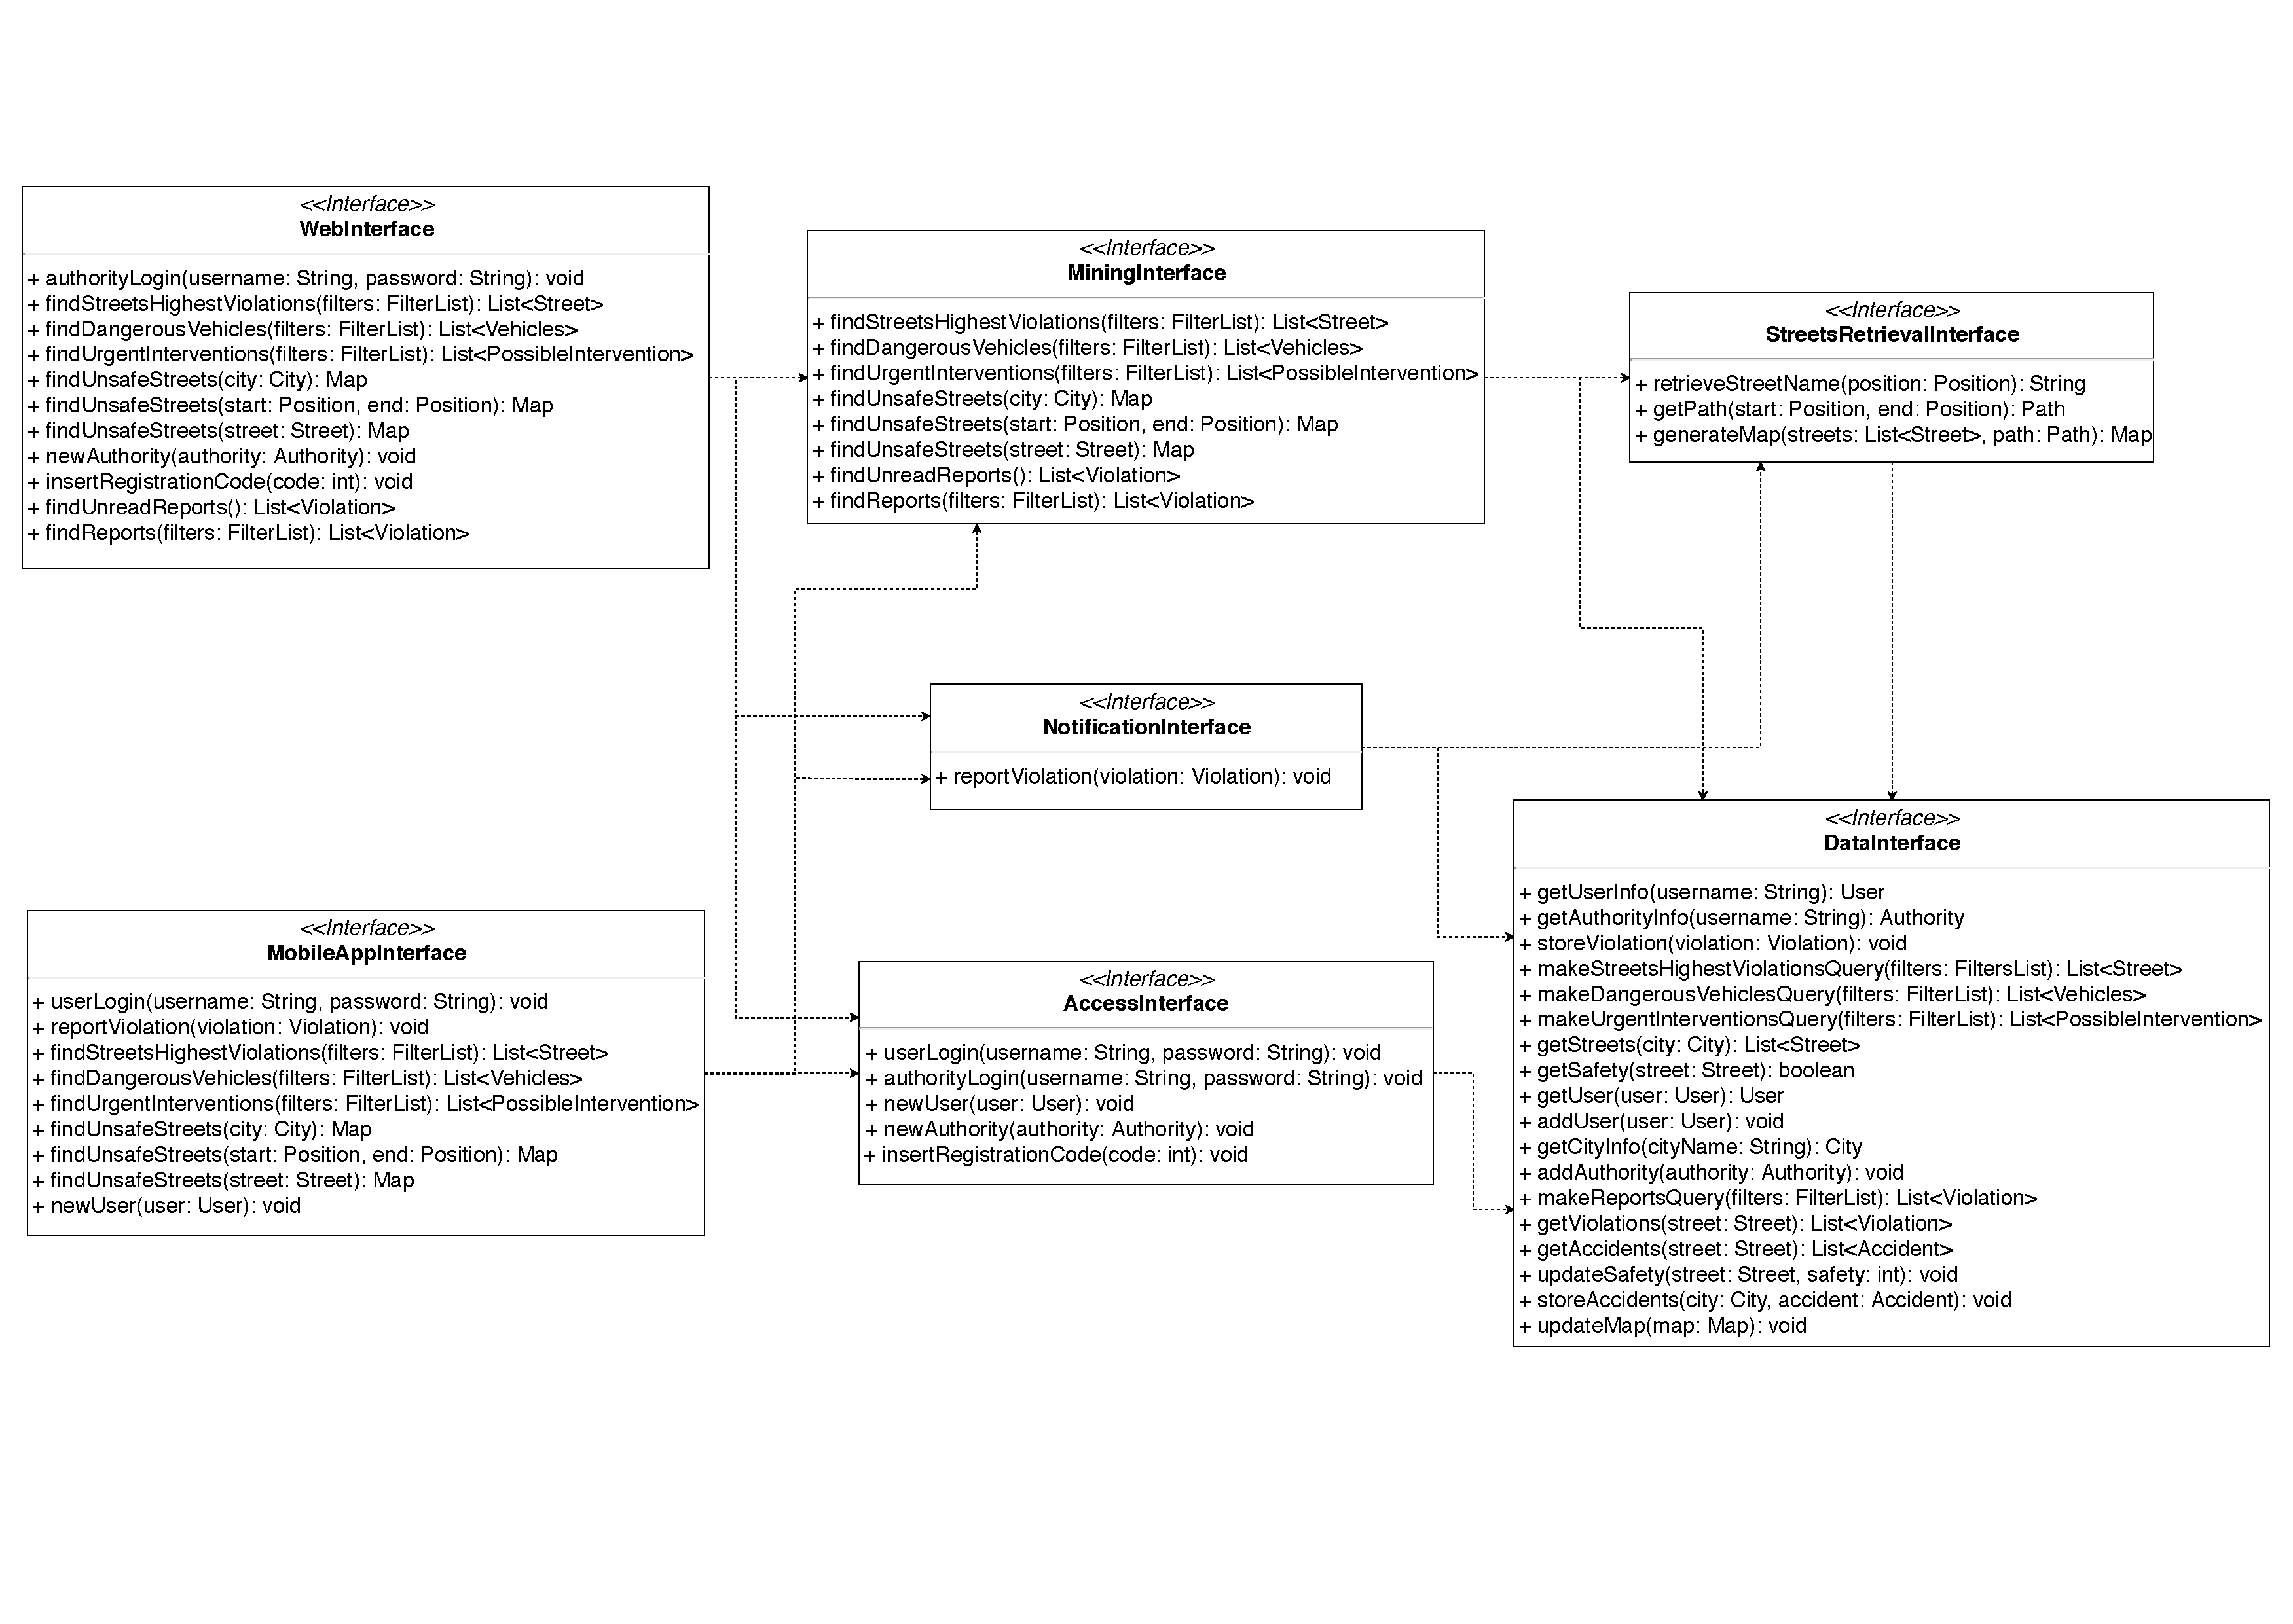
\includegraphics[scale=0.33, angle=90]{miscellaneous/componentInterfaces}
			\caption{\label{fig:componentInterfaces} Component Interfaces Diagram}
		\end{figure}
		
		\blueAutoref{fig:componentInterfaces} shows the component interfaces that are inside the application server. For every interface, the exposed methods are shown. Only the internal interfaces are shown. All the methods used in the sequence diagrams of the \hyperref[sec:runtimeView]{RuntimeView section} must be shown here. For what concerns the specific methods, their input parameters and returned value, they are only meant to give an idea of what they should do, but we are open to changes at the implementation level.
		
		\subsubsection[WebInterface]{\hyperlink{toc}{WebInterface}}
			This is the interface with all the methods exposed by the ClientHandler component that will be called by the WebServer. This methods have the only purpose of forwarding requests to the right component of our system that will handle them. The parameters and the returned values are the same as in the interfaces of the components to which the requests are forwarded to. Therefore, they won't be described here.
		
		\subsubsection[MobileAppInterface]{\hyperlink{toc}{MobileAppInterface}}
			Same as above, except that this interface is specific for the requests that come from the UserApp. Some methods are duplicated in these two interfaces because they realize functionalities that both users and authorities are supposed to get advantage of.
			
		\subsubsection[MiningInterface]{\hyperlink{toc}{MiningInterface}}
			The main purpose of the methods exposed in this interface is to prepare the queries that will be then forwarded to the DataManager component. Queries, that are the means through which mining functionality is provided by our system, usually have a bunch of filters that are here represented by the objects of type FilterList. It is a fictional Class that stands for a multitude of other classes: for example, a user can filter by City, Street, ViolationType and so on. Thus, we can imagine this object at the implementation level having some fields, that could be scalar in case of City, or arrays when users want to include some different types of violation in their queries. The unused fields (for example if a user doesn't want to filter by time slot) will be left empty, for example set to null. Other types of queries, implemented with the overloaded method findUnsafeStreets() for example, are a little bit more simple so the decision is to use the actual object used as parameters. findUnreadReports() and findReports() are actually quite similar: the first is a simpler version of the second because it has no filters as parameters and will include in the returned list of violations only those that have the "read" field set to false. 
		
		\subsubsection[NotificationInterface]{\hyperlink{toc}{NotificationInterface}}
			Despite the fact this interface only exposes one method, it is extremely important because it fulfills the reports notification functionality, that is the very core of our system. The idea is that the UserApp will create an object of type Violation and will then send it to the server and finally to this method, that is able to process it. This method will interact with IRI and MapManager to prepare the final Violation object that will be stored into the database.
		
		\subsubsection[AccessInterface]{\hyperlink{toc}{AccessInterface}}
			These methods are useful for registration and login purposes. They're actually quite simple and self-explanatory. The objects of types User and Authority have all the information gathered during the registration phase, and the methods newUser() and newAuthority() use them to store all the information in the database.
		
		\subsubsection[StreetsRetrievalInterface]{\hyperlink{toc}{StreetsRetrievalInterface}}
			The methods of this interface are exposed by the MapManager component, whose main purpose is to interact with the external MapInterface and for example ask for street names, paths and maps. Our system is not able to do all of this by itself, so this is the reason why we need an external interface like MapInterface. The objects of type Position are created either by getting the user's GPS positon through the GPS module of the user's device or when the user inserts the position manually. The generateMap() method requires a detailed explanation. It has two object as input, a list of object of type Street and a Path. Depending on the case, only one of those parameters will be set, while the other one will be left null. The goal of this method is handing all the necessary information to the MapInterface so that it could generate a colored map according to the streets safety data. Of course, if path option is selected by the user, the previously calculated path will have to be shown in the generated map and this is the reason why it appears as a parameter. In addition to this, an object of type Path already includes a list of the involved streets plus other information that is needed to link all the streets in a particular way (e.g. right and left turns etc.), therefore when a Path object is passed, generateMap() won't need the list of streets.
		
		\subsubsection[DataInterface]{\hyperlink{toc}{DataInterface}}
			This interface contains the methods exposed by the DataManager component. This component is in charge of communicating with the DBMS. In this way, the whole system is decoupled from the actual DBMS. All of these methods will be implemented by calling the methods exposed by the DBMS that are not modeled here for the sake of simplicity.
		
	
		\FloatBarrier
		
	\subsection[Selected Architectural Styles and Patterns]{\hyperlink{toc}{Selected Architectural Styles and Patterns}}
		\label{sec:selectedArchitecturalStylesAndPatterns}
		
		In this section we are going to describe precisely which are the architectural choices we did while designing the system and why we decided to choose them. As we saw in the deployment view section (\blueRef{sec:deploymentView}) we started with a \textbf{client-server} approach and then realized it with a \textbf{four-tier architecture}. We now need to describe why we decided these two styles that work good together but also how the elements that really deploy the system can communicate, hence we want also to describe precisely the communications that we highlighted in red in the deployment diagram (\blueAutoref{fig:deploymentDiagram}).
		
		\subsubsection[Client-Server]{\hyperlink{toc}{Client-Server}}
			\label{sec:clientServerDecision}
			
			Our system, as described in the context viewpoint of \blueAutoref{fig:contextViewpoint}, needs to interact with several external systems. It is true that in general SafeStreets needs to interact with systems that provide him services in order to realize its functionalities, but it is also true that SafeStreets aims to be a \textbf{crowd-sourced} system that is going to manage interactions with several users (who provide him the data) and several authorities. Thanks to these considerations, after studying different alternatives, we decided to choose a \textbf{client-server} architectural approach in order to easily manage the interaction with the mobile application of the users and to have a centralized server that is able to provide the services of the system to any customer that requires them.
			
			\vspace{0.3cm}
			
			\begin{figure}[h!]
				\centering
				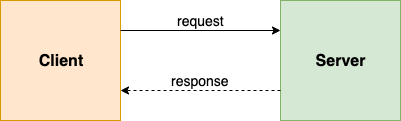
\includegraphics[scale=0.6]{architecture/clientServer.png}
				\caption{\label{fig:clientServerArchitecture} Client Server Architecture}
			\end{figure}

			Thanks to the client-server approach we also simplify the way in which we communicate with the external clients taking the decision of using the same technology of communication. In fact, as we will describe precisely in the further section \blueRef{sec:RESTDecision}, we are going to build our system in a RESTful way as we can have a simple communication protocol with HTTPS for the \textbf{Web Application} and we can integrate it with the \textbf{Mobile Application} in order to have the same APIs. This decision has several motivations even if it may not look the best choice to manage the interaction with the mobile application; the first is the one just presented related to the development and interfacing to a single API technology, another is connected with an implementation and integration aspect (as we will see in section \blueRef{sec:selectedArchitecturalStylesAndPatterns}) that is: as we can see in the plan identified by the diagram of \blueAutoref{fig:useRelationHierarchy} the implementation and integration (obviously testing too) of the \textbf{User App} and \textbf{Web Server} will take place in parallel. In this way, as we will need at this moment to define also the interfaces that provide the communication, we will develop first a common REST API on which the two different interfaces will specialize in order to connect to the related device.\\
			
			 The communications with the other systems depend on the services they provide, as we can see in the deployment diagram (\blueAutoref{fig:deploymentDiagram}) some of the services are still provided in a RESTful way while others, related in particular to the interaction with the \emph{database server} and the \emph{email server} consider instead a classic interfacing related to the management of data and the using of an email service.
			
		\subsubsection[Four Tier Architecture]{\hyperlink{toc}{Four Tier Architecture}}
			\label{sec:fourTierArchitectureDecision}
			
			Selected the \textbf{client-server} approach we needed to decide how to manage the layers of our system. We chose a multilayered architecture first to benefit of its advantages such as: decoupling, reuse, flexibility, migration... Second to have a way to realize a centralized business logic that allows to manage all the complex management of the data we need to take care of. Thanks to the different layers on which our system is designed we also separate the data as it can be managed more easily rather than having its complexity added inside our principal server. A multilayered architecture allows also to adopt the \textbf{thin-client} approach by letting only the presentation layer to be managed on the devices of the clients.\\
			
			For SafeStreets we decide to choose a \textbf{Four Tier Architecture} as we need to take into account (as we see from the devices highlighted in the deployment diagram of \blueAutoref{fig:deploymentDiagram}) two different approaches for the client interaction: \textbf{mobile application} for the users and \textbf{web application} for the authorities. Hence the necessity of a Web Server needs also to be considered in order to manage the web side of the clients. For this first architectural decision of the client's separation and to maintain the \textbf{thin-client} approach we need to have two different tiers to handle the \textbf{Presentation Layer}. In order to consider the management of the information (fundamental resource for our crowd source based system) we also need to separate the business logic from the data. The two remaining layers will be separated, hence one tier is needed to deal with the \textbf{Logic Layer} and another for the \textbf{Data Layer}.\\
			
			We now present once more the picture of our four tier system as we can easier compare it with what we have just said.
			
			\begin{figure}[h!]
				\centering
				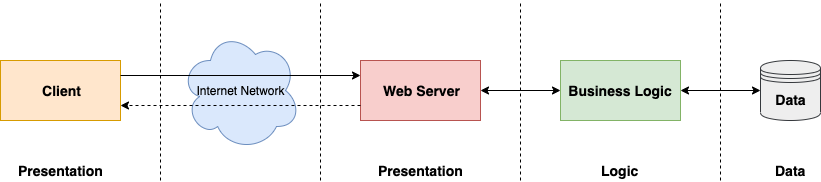
\includegraphics[scale=0.4]{architecture/fourTierArchitecture.png}
				\caption{Four Tier Architecture}
			\end{figure}
		
			To be completely precise, our system would also need an additional tier, on which the \textbf{script engine server} would be running. This layer would allow to manage the dynamic generation of  the web pages for the authority web app. To focus on the most critical aspects of the design process we decided not to represent also this layer to keep quite simple diagrams and descriptions. However we should not completely overlook this consideration as it may be needed in particular for the generation of the map in the \emph{Unsafe Streets} functionality.
			
		\subsubsection[RESTful Architecture]{\hyperlink{toc}{RESTful Architecture}}
			\label{sec:RESTDecision}
			
			We have already motivated the choice of this approach in the client-server section (\blueRef{sec:clientServerDecision}) in particular for how our system is going to provide its services to the clients. The communications with the external services do not need a precise motivation, we only need to stick with the decisions of the system that is providing the functionality and adapt our communication modules.\\
			
			Now we want to present some further motivations and advantages that the RESTful architecture allows us to obtain. The principle on which REST is based, that is the stateless interaction of requests between the clients and server, is really helpful to us in order to manage the huge amount of data we expect to receive for the notification process. As we have already said, in this way, we will be also able to manage both the requests coming from the users and the authorities with one single interface that is adapted for the \textbf{mobile application} side and the \textbf{web application} side.\\
			
			In conclusion this communication architecture based on HTTP is perfectly embraced in our four tier architecture and allows also an easier way to manage the information in a precise standard. In particular we expect the JSON format of the result provided by the \textbf{Map Interface} when it return us the data relative to the map that has to be displayed to our clients for the \emph{Unsafe Streets} functionality.
	
	\subsection[Other Design Decisions]{\hyperlink{toc}{Other Design Decisions}}
		\label{sec:otherDesignDecisions}						
		
		In this subsection we want to provide additional details on what we have presented in the entire section. In particular we will focus on the motivations for the \textbf{relational database} chosen and on a brief description of the two approaches used to realize a \textbf{native mobile application}.
		
		\subsubsection[Relational Database Approach]{\hyperlink{toc}{Relational Database Approach}}
			\label{sec:relationaldbApproach}
			
			We decided to consider a relational approach in particular for the way in which the data has to be managed because of the functionalities of the system. In fact, without focusing on the clients that can be managed in a relational database without any problem, we have seen how several relations are established between the entities that compose our system. In particular the most important are the ones related to the safety computation: first the relations between the interventions and the streets and also between the accidents and the streets allow to determine the safety; second the relations between the \textbf{safety} and the street allows us to process this data and send it to the clients as it can be highlighted for the \emph{Unsafe Streets} functionality.\\
			
			Considering now some more implementation aspects, as we can also see in the decision tree (\blueAutoref{fig:decisionTree}), we decided to choose MySQL as the DBMS to interact with because it is the most popular relational one and provides a complete and clear documentation on how to benefit of its services.
			
		\subsubsection[Native Application Approach]{\hyperlink{toc}{Native Application Approach}}
			\label{sec:nativeAppApproach}
			
			We decided to consider a native approach for the development of the \textbf{mobile application} for the users in order to provide a better experience of interaction with the system but also to obtain the best communication and responsiveness between the client and the server. Nowadays the mobile applications are developed with two different languages depending on the OS of the device: for \textbf{Android} we will use \emph{Android Studio} while for \textbf{IOS} the native language \textbf{Swift}.
			
			\paragraph{Android Studio} it is the official IDE for Google's Android operating system, designed specifically for Android development. It is available for every operating system and perfectly documented with a huge community. In addition it is based on \emph{Gradle} that helps a lot in the dependency management and thus makes our result more extensible. In fact, it is important to remark that we are designing an extensible system: as we saw in the \textbf{class-diagram} of the RASD \cite{RASD} the most expected extension we expect is the possibility to report not just parking violations but also other kinds of the general traffic violations.
			
			\paragraph{Swift} it is the official programming language developed by Apple in order to replace the old Objective-C paradigm on which all the IOS applications were based on. It is designed to work with the most popular Apple's frameworks and provides several performances and safety trade-offs. We choose it as the native approach to develop a mobile application for IOS as it is still highly documented and its community is getting bigger and bigger.